\documentclass[10pt,a4paper]{amsart}
\usepackage{fontspec}  
\usepackage[utf8]{inputenc}
\usepackage[english]{babel}
\usepackage[mathcal]{euscript}
\usepackage{mathrsfs}  
\usepackage{amsmath}
\usepackage{amsfonts}
\usepackage{mathrsfs}  
\usepackage{amssymb}
\usepackage{stmaryrd}
\usepackage{graphicx}
\usepackage{mathtools}
\usepackage{pgfplots}
\usepackage{xfrac}
\usepackage{listings}
\usepackage{xcolor}
\usepackage{lstlinebgrd}
\usepackage{ebproof}
\usepackage{graphicx,float}
\usepackage[colorlinks=true, linkcolor=cyan, urlcolor=cyan, citecolor=cyan]{hyperref}
\usepackage[shortlabels]{enumitem}
\usepackage[textsize=tiny,textwidth=45]{todonotes}

\newcommand{\klcomp}{\star}
\newcommand{\parI}{\mathop{\bowtie}}
\newcommand{\seqI}{\mathop{\triangleright}}
\DeclareMathOperator{\demon}{\square}
\DeclareMathOperator{\angel}{\Diamond}
\makeatletter
\DeclareRobustCommand{\iscircle}{\mathord{\mathpalette\is@circle\relax}}
\newcommand\is@circle[2]{%
  \begingroup
  \sbox\z@{\raisebox{\depth}{$\m@th#1\bigcirc$}}%
  \sbox\tw@{$#1\square$}%
  \resizebox{!}{\ht\tw@}{\usebox{\z@}}%
  \endgroup
}
\makeatother
\DeclareMathOperator{\statt}{\iscircle_\prog{p}}
\newcommand{\schfont}[1]{\mathcal{#1}}
\newcommand{\sch}{\schfont{S}}
\newcommand{\conv}[1]{\mathrm{conv}\, {#1}}
%%%%%%%%%%%%% Macros
\newcommand{\renato}[1]{\textcolor{teal}{RN Note: #1}}
\newcommand{\codiag}{\triangledown}
%%%% Categories
\newcommand{\catfont}[1]{\mathsf{#1}}
\newcommand{\cop}{\catfont{op}}
\newcommand{\Law}{\catfont{Law}}
\newcommand{\catV}{\catfont{V}}
\newcommand{\catX}{\catfont{X}}
\newcommand{\catC}{\catfont{C}}
\newcommand{\catCat}{\catfont{C}}
\newcommand{\catCop}{\catfont{C^{op}}}
\newcommand{\catD}{\catfont{D}}
\newcommand{\catE}{\catfont{E}}
\newcommand{\catA}{\catfont{A}}
\newcommand{\catB}{\catfont{B}}
\newcommand{\catP}{\catfont{P}}
\newcommand{\catMet}{\catfont{Met}}
\newcommand{\catCPTP}{\catfont{CPTP}}
\newcommand{\catCPS}{\catfont{CPS}}
\newcommand{\catCP}{\catfont{CP}}
\newcommand{\catQ}{\catfont{Q}}
\newcommand{\catSet}{\catfont{Set}}
\newcommand{\catFinSet}{\catfont{FinSet}}
\newcommand{\catPO}{\catfont{PO}}
\newcommand{\catCompFunc}{\catfont{CompFunc}}
\newcommand{\catBan}{\catfont{Ban}}
\newcommand{\catVect}{\catfont{CVect}}
\newcommand{\WstarCPSU}{\catfont{Wstar_{CPSU}}}
\newcommand{\WstarCPSUop}{\left(\catfont{Wstar_{CPSU}}\right)^{\catfont{op}}}
\newcommand{\catI}{\catfont{I}}
\newcommand{\Set}{\catfont{Set}}
\newcommand{\Top}{\catfont{Top}}
\newcommand{\Pos}{\catfont{Pos}}
\newcommand{\Inj}{\catfont{Inj}}
\newcommand{\Det}{\catfont{RMhat}}
\newcommand{\CoAlg}[1]{\catfont{CoAlg}\left (#1 \right )}
\newcommand{\Mon}{\catfont{Mon}}
\newcommand{\Mnd}{\catfont{Mnd}(\catC)}
\newcommand{\SMnd}{\catfont{Mnd}(\Set)}
\newcommand{\CLat}{\catfont{CLat}}
\newcommand{\SLat}{\catfont{SLat}}
\newcommand{\Stone}{\catfont{Stone}}
\newcommand{\Spectral}{\catfont{Spectral}}
\newcommand{\CompHaus}{\catfont{CompHaus}}
\newcommand{\Subs}[2]{\catfont{Sub}_{}}
\newcommand{\Cone}{\catfont{Cone}}
\newcommand{\LCone}{\catfont{LCone}}
\newcommand{\StComp}{\catfont{StablyComp}}
\newcommand{\PosC}{\catfont{PosComp}}
\newcommand{\Haus}{\catfont{Haus}}
\newcommand{\Meas}{\catfont{Meas}}
\newcommand{\Coh}{\catfont{CohDom}}
\newcommand{\Ord}{\catfont{Ord}}
\newcommand{\Dcpo}{\catfont{DCPO}}
\newcommand{\Dom}{\catfont{Dom}}
\newcommand{\EndoC}{[\catC,\catC]}
\newcommand{\Dcpop}{\catfont{DCPO}^\catfont{p}}
%% General functors
\newcommand{\funfont}[1]{#1}
\newcommand{\funF}{\funfont{F}}
\newcommand{\funU}{\funfont{U}}
\newcommand{\funG}{\funfont{G}}
\newcommand{\funT}{\funfont{T}}
\newcommand{\funI}{\funfont{I}}
%% Particular kinds of functors
\newcommand{\sfunfont}[1]{\mathrm{#1}}
\newcommand{\Pow}{\sfunfont{P}}
\newcommand{\PP}{\sfunfont{V}}
\newcommand{\Dist}{\sfunfont{V}_{=1,\omega}}
\newcommand{\PDist}{\sfunfont{V}_{\leq 1,\omega}}
\newcommand{\Maybe}{\sfunfont{M}}
\newcommand{\List}{\sfunfont{L}}
\newcommand{\UForg}{\sfunfont{U}}
\newcommand{\Forg}[1]{\sfunfont{U}_{#1}}
\newcommand{\Id}{\sfunfont{Id}}
\newcommand{\Vie}{\sfunfont{V}}
\newcommand{\Disc}{\funfont{D}}
\newcommand{\Weight}{\sfunfont{W}}
\newcommand{\homf}{\sfunfont{hom}}
\newcommand{\Yoneda}{\sfunfont{Y}}
%% Diagram functors
\newcommand{\Diag}{\mathscr{D}}
\newcommand{\KDiag}{\mathscr{K}}
\newcommand{\LDiag}{\mathscr{L}}
%% Monads
\newcommand{\monadfont}[1]{\mathbb{#1}}
\newcommand{\monadT}{\monadfont{T}}
\newcommand{\monadS}{\monadfont{S}}
\newcommand{\monadU}{\monadfont{U}}
\newcommand{\monadH}{\monadfont{H}}
\newcommand{\str}{\mathrm{str}}
%% Adjunctions
\newcommand\adjunct[2]{\xymatrix@=8ex{\ar@{}[r]|{\top}\ar@<1mm>@/^2mm/[r]^{{#2}}
& \ar@<1mm>@/^2mm/[l]^{{#1}}}}
\newcommand\adjunctop[2]{\xymatrix@=8ex{\ar@{}[r]|{\bot}\ar@<1mm>@/^2mm/[r]^{{#2}}
& \ar@<1mm>@/^2mm/[l]^{{#1}}}}
%% Retractions
\newcommand\retract[2]{\xymatrix@=8ex{\ar@{}[r]|{}\ar@<1mm>@/^2mm/@{^{(}->}[r]^{{#2}}
& \ar@<1mm>@/^2mm/@{->>}[l]^{{#1}}}}
%% Limits
\newcommand{\pv}[2]{\langle #1, #2 \rangle}
\newcommand{\limt}{\mathrm{lim}}
\newcommand{\pullbackcorner}[1][dr]{\save*!/#1+1.2pc/#1:(1,-1)@^{|-}\restore}
\newcommand{\pushoutcorner}[1][dr]{\save*!/#1-1.2pc/#1:(-1,1)@^{|-}\restore}
%% Colimits
\newcommand{\colim}{\mathrm{colim}}
\newcommand{\inl}{\mathrm{inl}}
\newcommand{\inr}{\mathrm{inr}}
%% Distributive categories
\newcommand{\distr}{\mathrm{dist}}
\newcommand{\undistr}{\mathrm{undist}}
%% Closedness
\newcommand{\curry}[1]{\mathrm{curry}{#1}}
\newcommand{\app}{\mathrm{app}}
%% Misc. operations
\newcommand{\const}[1]{\underline{#1}}
\newcommand{\comp}{\cdot}
\newcommand{\id}{\mathrm{id}}
\newcommand{\sw}{\mathrm{sw}}
\newcommand{\spt}{\mathrm{sp}}
\newcommand{\sh}{\mathrm{sh}}
\newcommand{\jn}{\mathrm{jn}}
\newcommand{\dist}{\mathrm{dist}}
\newcommand{\unfold}{\mathrm{unfold}}
\newcommand{\fold}{\mathrm{fold}}
%% Factorisations
\newcommand{\EClass}{E}
\newcommand{\MClass}{M}
\newcommand{\MConeClass}{\mathcal{M}}
%%%%%%%%%%%%%%%% End of Categorical Stuff

%%%% Misc
%% Operations
\newcommand{\blank}{\, - \,}
\newcommand{\sem}[1]{\left \llbracket #1 \right \rrbracket}
\newcommand{\asem}[1]{ \llparenthesis #1 \rrparenthesis}
\newcommand{\closure}[1]{\overline{#1}}
\DeclareMathOperator{\img}{\mathrm{im}}
\DeclareMathOperator{\dom}{\mathrm{dom}}
\DeclareMathOperator{\codom}{\mathrm{codom}}
%% Sets of numbers
\newcommand{\Nats}{\mathbb{N}}
\newcommand{\Reals}{\mathbb{R}}
\newcommand{\Rats}{\mathbb{Q}}
\newcommand{\Rz}{\Reals_{\geq 0}}
\newcommand{\Complex}{\mathbb{C}}
%% Writing
\newcommand{\cf}{\emph{cf.}}
\newcommand{\ie}{\emph{i.e.}}
\newcommand{\eg}{\emph{e.g.}}
\newcommand{\df}[1]{\emph{\textbf{#1}}}
%%%%%%%%%%%%%%%% End of Misc

%%%% Programming Stuff
%% Types
\newcommand{\typefont}[1]{\mathbb{#1}}
\newcommand{\typeOne}{1}
\newcommand{\typeTwo}{2}
\newcommand{\typeA}{\typefont{A}}
\newcommand{\typeB}{\typefont{B}}
\newcommand{\typeC}{\typefont{C}}
\newcommand{\typeV}{\typefont{V}}
\newcommand{\typeD}{\typefont{D}}
\newcommand{\typeE}{\typefont{E}}
\newcommand{\typeF}{\typefont{F}}
\newcommand{\typeI}{\typefont{I}}
%% RuleName
\newcommand{\rulename}[1]{(\mathrm{#1})}
%% Sequents
\newcommand{\jud}{\vdash}
\newcommand{\vljud}{\triangleright}
\newcommand{\cojud}{\vdash_{\co}}
\newcommand{\vl}{\mathtt{v}}
\newcommand{\co}{\mathtt{c}}
% Program font
\newcommand{\prog}[1]{\ensuremath{\tt #1}}
\newcommand{\blue}[1]{\textcolor{blue}{#1}}
\newcommand{\pseq}[3]{#1 \leftarrow #2; #3}
\newcommand{\ppm}[4]{(#1,#2) \leftarrow #3; #4}
\newcommand{\pinl}[1]{\prog{inl}(#1)}
\newcommand{\pinr}[1]{\prog{inr}(#1)}
\newcommand{\pcase}[5]{\prog{ case } #1 \prog{ \hspace{2pt} of \hspace{2pt} } \pinl{#2} \Rightarrow #3 ; \pinr{#4} \Rightarrow #5}
%% Sets of terms
\newcommand{\ValuesBP}[2]{\mathsf{Values}(#1, #2)}
\newcommand{\TermsBP}[2]{\mathsf{Terms}(#1, #2)}
\newcommand{\closValP}[1]{\ValuesBP{\emptyset}{#1}}
\newcommand{\closTermP}[1]{\TermsBP{\emptyset}{#1}}
\newcommand{\closVal}{\closValP{\typeA}}
\newcommand{\closTerm}{\closTermP{\typeA}}
%% Contextual equivalence
\newcommand{\ctxeq}{\equiv_{\prog{ctx}}}

%%%% End of Programming Stuff
\newcommand{\Shuff}{\mathrm{Sf}}

%%%% Domain theory
\newcommand{\upclos}{\mathord{\uparrow}}
\newcommand{\dwclos}{\mathord{\downarrow}}

%%%% Quantum stuff
\newcommand{\Hilb}{\catfont{Hilb}}
\newcommand{\tr}{\text{Tr}}

%%%% Norms
\newcommand{\euclideannorm}[1]{\left\lVert #1  \right\rVert_{2}}
\newcommand{\spectralnorm}[1]{\left\lVert #1  \right\rVert_{\infty}}
\newcommand{\tracenorm}[1]{\left\lVert #1  \right\rVert_{1}}
\newcommand{\diamondnorm}[1]{\left\lVert #1  \right\rVert_{\diamondsuit}}
\newcommand{\lonenorm}[1]{\left\lVert #1  \right\rVert_{ L^{1} }}
\newcommand{\gentracenorm}[1]{\left\lVert #1  \right\rVert_{ L^\infty }}
\newcommand{\gendiamondnorm}[1]{\left\lVert #1  \right\rVert_{ \diamondsuit \text{ gen}}}
\newcommand{\opnorm}[1]{\left\lVert #1  \right\rVert_{\text{op}}}
\newcommand{\norm}[1]{\left\lVert #1  \right\rVert}
\newcommand{\cbnorm}[1]{\left\lVert #1  \right\rVert_{\text{cb}}}
\newcommand{\projnorm}[1]{\left\lVert #1  \right\rVert_{\pi}}

%%%% Tensor
\newcommand{\projtensor}{\widehat{\otimes}_\pi}

\usepackage[left=2cm,right=2cm,top=2cm,bottom=2cm]{geometry}
\usepackage{tcolorbox}
\usepackage{braket}
\usepackage{quantikz}
\usepackage{tikz-cd}
\usepackage{mathabx}
\linespread{1.10}
\author{\dots}
\title{Notes}
\pgfplotsset{compat=1.18}

\lstset{
language=C,
showstringspaces=false,
keywordstyle=\color{blue},
basicstyle=\fontsize{10}{13}\ttfamily,
emph={exit,blue,unif,then,wait},emphstyle=\color{blue},
breaklines=true,
escapeinside={*@}{*@}
}


\usepackage{proof}
\usepackage{amsthm}
\usepackage[all]{xy}
%for definition
\theoremstyle{definition}
\newtheorem{definition}{Definition}[section]

%for examples
\theoremstyle{definition}
\newtheorem{example}[definition]{Example}

%lemmas
\theoremstyle{definition}
\newtheorem{lemma}[definition]{Lemma}

%proposition
\theoremstyle{definition}
\newtheorem{proposition}[definition]{Proposition}
%corollary
\theoremstyle{definition}
\newtheorem{corollary}[definition]{Corollary}

%theorem
\theoremstyle{definition}
\newtheorem{theorem}[definition]{Theorem}

% Renato's macros
\newcommand{\until}{\> \textcolor{blue}{\prog{for}} \>}
\newcommand{\then}{\textcolor{blue}{then}}
\newcommand{\progife}[3]{{ \blue{\prog{if}} \> #1 \> \blue{\prog{then}} \> 
{\prog #2} \> \blue{\prog{else}} \> {\prog #3}}}
\newcommand{\progwhile}[2]{{\blue{\prog{while}} \>  #1 \> \blue{\prog{do}} \> \{ \> {#2}  \> \}}}
\newcommand{\scomp}{\, \blue{;} \,}
\newcommand{\prem}[1]{(\text{if\/ }#1)}
\newcommand{\nline}{\vspace{-5mm}}
\newcommand{\ssto}[1][]{~\to^{#1}~}
\newcommand{\bsto}{~\Downarrow~}
\newcommand{\stp}{\mathit{stop}}
\newcommand{\skp}{\mathit{skip}}
\newcommand{\err}{\mathit{err}}
\providecommand{\comma}{,\operatorname{}\linebreak[1]}		% possibly line-beaking comma
\newcommand{\sep}{\kern1pt\comma\kern-1pt}
\newcommand{\lrule}[3]{\textbf{#1}\quad\frac{#2}{#3}}
\newcommand{\ptt}{{\prog tt}}
\newcommand{\pff}{{\prog ff}}
\newcommand{\unif}{{\prog \blue{unif}}}
\newcommand{\meas}[1]{\mathcal{M}(#1)}
\newcommand{\pmap}{ \xrightharpoonup{\hspace{0.1cm}} }

\begin{document}
\title{Quantum stuff}
\maketitle
%\tableofcontents
\section{Lambda-calculus with conditionals}

\subsection{Syntax}

Considering a class $G$ of ground types, the grammar of types for linear lambda calculus with conditionals corresponds to:

\begin{equation*} \label{eq:grammartypes}
  \centering
   \typeA ::= X \in G \hspace{3 pt} \vert \hspace{3 pt} \typeI \hspace{3 pt}  \vert \hspace{3 pt} \typeA  \otimes  \typeA \hspace{3 pt} \vert  \hspace{3 pt} \typeA  \oplus \typeA \hspace{3 pt}  \vert  \hspace{3 pt} \typeA \multimap  \typeA
  \end{equation*}

The term formation rules for conditionals are depicted in \autoref{fig:typing_rules_cond}. 

\begin{figure}[H]
    \begin{equation*}
    \begin{aligned}
    &\hspace{10pt}
    %
    \begin{prooftree}
        \hypo{\Gamma \vljud v: \typeA}
        \infer1[(inl)]{\Gamma \vljud \inl_{\typeB}(v): \typeA \oplus \typeB}
    \end{prooftree}
    %
    \hspace{30pt}
    %
    \begin{prooftree}
        \hypo{\Gamma \vljud v: \typeB}
        \infer1[(inr)]{\Gamma \vljud \inr_{\typeA}(v): \typeA \oplus \typeB}
    \end{prooftree} 
    %
    \\[20pt]
    &\hspace{-20pt}
    %
    \begin{prooftree}
        \hypo{\Gamma \vljud v: \typeA \oplus \typeB}
        \hypo{\Delta, x: \typeA \vljud w: \typeD}
        \hypo{\Delta, y: \typeB \vljud u: \typeD}
        \hypo{E \in \Shuff(\Gamma; \Delta)}
        \infer4[(case)]{E \vljud \text{case } v\,
        \{\inl_{\typeB}(x) 
            \Rightarrow w ; \,
          \inr_{\typeA}(y) \Rightarrow u
        \}: \typeD}
    \end{prooftree}
    %
    \\[10pt]
    \end{aligned}
    \end{equation*}
    \caption{Term formation rules for conditionals}
    \label{fig:typing_rules_cond}
\end{figure}
The rules presented in Figure \ref{fig:typing_rules_cond} enjoy the following
properties.

\begin{theorem} \label {theorem:unique_der}
   Lambda calculus with conditionals has the following properties:
   \begin{enumerate}
     \item\label{perm} for all judgements $\Gamma \vljud v$ and $\Gamma'
             \vljud v$, te($\Gamma$) $\simeq_{\pi}$  te($\Gamma'$); 
     %
     \item\label{type} additionally if $\Gamma \vljud v: \typeA,
       \Gamma' \vljud v: \typeA'$, and $\Gamma \simeq_{\pi}
       \Gamma'$, then $\typeA$ must be equal to $\typeA'$;
     %
     \item\label{der} all judgements $\Gamma \vljud v:\typeA$ have a unique derivation.
\end{enumerate}
\end{theorem}
%
\begin{proof}
It follows in all three cases from induction over the length of derivation
trees. 

Let us focus first on Property~\eqref{perm}. The case of the rules concerning
injections is direct. As for rule~$\rulename{cond}$ take two contexts $E$ and
$E'$ for the same conditional. According to this rule we obtain contexts
$\Gamma$, $\Gamma'$, $\Delta$, $\Delta'$ such that $E \in
\Shuff(\Gamma;\Delta)$ and $E' \in \Shuff(\Gamma';\Delta')$. It follows from
induction that  $\Gamma \simeq_\pi \Gamma'$ and $\Delta \simeq_\pi \Delta'$,
and the proof is then obtained from the sequence of equivalences,
\begin{align*}
        \text{te}(E) & \simeq_\pi \text{te}(\Gamma, \Delta) 
        \\
        & \simeq_\pi \text{te}(\Gamma', \Delta')
        \\
        & \simeq_\pi \text{te}(E')
\end{align*}
Concerning Property~\eqref{type}, the case of the rules concerning injections
is direct and the case of rule~$\rulename{cond}$ is a corollary of
Property~\eqref{perm}. Finally let us consider Property~\eqref{der}. Again the
case concerning injections is direct and we thus focus only on
rule~$\rulename{cond}$. According to this rule we obtain contexts $\Gamma$,
$\Gamma'$, $\Delta$, $\Delta'$ such that $E \in \Shuff(\Gamma;\Delta)$ and $E
\in \Shuff(\Gamma';\Delta')$. By an appeal to Property~\eqref{perm} we also
obtain $\Gamma \simeq_\pi \Gamma'$ and $\Delta \simeq_\pi \Delta'$, and thus
since shuffling preserves relative orders we obtain $\Gamma = \Gamma'$ and
$\Delta = \Delta'$. The proof then follows by induction.
\end{proof}

\begin{lemma}[Exchange and Substitution]
\label{lem:exh_and_sub} 
For every judgement $\Gamma,x: \typeA, y: \typeB, \Delta \vljud v: \typeD$ the
judgement $\Gamma, y:\typeB, x:\typeA, \Delta \vljud v:
\typeD$ is derivable. Not only this, given judgements  $\Gamma,x:\typeA \vljud
v: \typeB$ and $\Delta \vljud w: \typeA$ the judgement $\Gamma, \Delta \vljud
v[w/x]: \typeB$ is also derivable.
\end{lemma}


\begin{proof}
We start with the exchange property which follows by induction over the length
of derivation trees. The rules that involve injections are direct.  The rule
$\rulename{case}$ calls for case distinction, more specifically we  distinguish
between the cases in which both variables ($x : \typeA$ and $y : \typeB$) are
in $\Gamma$, both are in $\Delta$, and otherwise. The first two cases follow
straightforwardly by induction and the definition of a shuffle. For the third
case consider a judgement $E_1,x : \typeA, y : \typeB, E_2 \vljud \text{case }
v\, \{\inl_{\typeF}(a) \Rightarrow w ; \, \inr_{\typeE}(b) \Rightarrow u \}:
\typeD$, and assume with no loss of generality that $\Gamma$ is of the form
$\Gamma_1, x : \typeA, \Gamma_2$ and $\Delta$ of the form $\Delta_1, y :
\typeB, \Delta_2$. The proof now follows directly from the implication,
\[
        E_1, x : \typeA, y : \typeB, E_2 \in \Shuff(\Gamma_1, x : \typeA, \Gamma_2 ; \,
        \Delta_1, y : \typeB, \Delta_2)
        \Longrightarrow
        E_1, y : \typeB, x : \typeA, E_2 \in \Shuff(\Gamma_1, x : \typeA, \Gamma_2 ; \,
        \Delta_1, y : \typeB, \Delta_2)
\]
(which holds by the definition of a shuffle).

Finally we now focus on the substitution rule which also follows by induction over the
length of derivation trees. Again the cases involving the injections are direct,
and we thus only detail the proof of rule $\rulename{case}$. Consider then
judgements $E,x : \typeA \vljud \text{case } v\, \{\inl_{\typeD}(a) \Rightarrow
w ; \, \inr_{\typeE}(b) \Rightarrow u \}: \typeB$ and
$Z \vljud t : \typeA$ with $E \in \Shuff(\Gamma; \Delta)$. According to the definition
of a shuffle either $\Gamma$ is of the form $\Gamma_1, x: \typeA$ or $\Delta$ is
of the form $\Delta_1, x : \typeA$. The first case follows directly and the second case
is a corollary of the exchange rule.
\end{proof}

The equational system for the conditionals is shown in Figure
\ref{fig:equations-in-context-cond}.


  \begin{figure}[h!]
    \centering
    \begin{tcolorbox}[colframe=black, colback=white, boxrule=0.6pt, arc=1pt,boxsep=1pt,top=1pt,bottom=1pt, width=0.85 \textwidth]
    \begin{equation*}
        \begin{split}
          &(\beta_{case}^{inl}) \hspace{3pt} \text{case } 
          \inl_{\typeB}(v)\, \{ \inl_{\typeB} (x) \Rightarrow w 
          ;\, \inr_{\typeA} (y) 
          \Rightarrow u\}= w[v/x]
          %
          \\
          %
          &(\beta_{case}^{inr}) \hspace{3pt} \text{case } 
          \inr_{\typeA}(v)\, \{ \inl_{\typeB} (x) \Rightarrow w 
          ;\, \inr_{\typeA} (y) 
          \Rightarrow u\}= u[v/y]
          %
          \\
          %
          %
          & (\eta_{case}) \hspace{3pt} \text{case } v\, \{\text{inl}_{\typeB} (y) \Rightarrow w [ \text{inl}_{\typeB}(y)/x] ;\, \text{inr}_{\typeA} (z) \Rightarrow w [ \text{inr}_{\typeA}(z)/x]\} = w[v/x] 
        \end{split}
    \end{equation*}
    \end{tcolorbox}
    \caption{Equational system for the conditionals}
    \label{fig:equations-in-context-cond}
    \end{figure}


\subsubsection{Linear $\lambda$-calculus and quantum computation} \label{subsec:syntax_qc}

We now illustrate the use of the previous language for describing quantum
programs. To this effect, we first consider a type \emph{qbit} of qubits, the
basic unit of information in quantum computation. We then regard $\typeI \oplus
\typeI$ to be the type of bits, a common approach not only in quantum
computation~\cite{selinger04} but also in the categorical interpretation of a
`truth-values' object~\cite{johnstone02,cho15}. Next we propound the following
basic quantum operations:  the conversion of a bit into a qubit, $q : \typeI
\oplus \typeI  \to \emph{qbit}$, the measurement of a qubit,
$\emph{meas}:\emph{qbit} \to \typeI \oplus \typeI$, and a pre-determined set of
operations on $n$-qubits, $\emph{U}:\emph{qbit},\ldots,\emph{qbit} \to
\emph{qbit}^{\otimes n}$ and $\emph{CPTP}:\emph{qbit},\ldots,\emph{qbit} \to
\emph{qbit}^{\otimes n}$ . The latter includes unitary operations, as the Hadamard
gate $H : \emph{qbit} \to \emph{qbit}$, the not-gate $X : \emph{qbit} \to
\emph{qbit}$, and the cnot-gate $CNOT : \emph{qbit},\emph{qbit} \to
\emph{qbit}^{\otimes 2}$, and the former set operations such as the dephasing with probability $p$, $D_p : \emph{qbit},\emph{qbit} \to
\emph{qbit}^{\otimes 2}$. We consider as well a pre-determined set of quantum
states $\ket{\psi} : \typeI \to \emph{qbit}$.  Finally note that the values
\emph{true} and \emph{false} (in the type $\typeI \oplus \typeI$) are regarded to be 
the terms $\inl(\ast)$ and $\inr(\ast)$ respectively.


Let us now apply this machinery to two well-known problems in quantum computation
and quantum information.

\begin{example}[Coin toss] \label{ex:coin_toss_syntax}



In the quantum setting, tossing a `fair' coin can be described as preparing a qubit in a superposition of two states, $\ket{0}$ and $\ket{1}$, representing `heads' and `tails', each with an equal probability of $0.5$ and then measuring it. This is achieved by simply applying a Hadamard gate to the initial state $\ket{0}$, followed by a measurement.
More generally, tossing a coin (whether `fair' or `unfair') can be described as preparing a qubit in a superposition of  $\ket{0}$ and $\ket{1}$, with probabilities $p$ and $1-p$, respectively,  and then measuring it.  Considering $p= \cos(\theta/2)^2$ and the standard quantum gate operation $R_{y,\theta} : \emph{qbit} \to \emph{qbit}$,  this process is described by the following $\lambda$-term:

\begin{align*}
  &\textbf{CoinToss} = - \vljud \emph{meas} (R_{y,\theta} (\ket{0})): \typeI \oplus \typeI
\end{align*}


\end{example}

\begin{example}[Quantum state discrimination] \label{ex:quantum_state_discrimination_syntax}

Quantum state discrimination is a pivotal challenge in quantum information,
fundamental to the extraction of classical information from quantum systems.
While orthogonal states can be perfectly distinguished, the same does not apply
to nonorthogonal states. In fact even when the set of possible nonorthogonal
states is known, determining the optimal discrimination strategy is considered
a nontrivial problem.

When distinguishing between two nonorthogonal quantum states, the Helstrom
measurement represents the optimal strategy
\cite{helstromQuantumDetectionEstimation1976}. In the case where both states
are pure, the Helstrom measurement corresponds to a projective measurement
\cite{barnett2009quantum}.  When operating within the computational basis, a
projective measurement can be understood as the application of a unitary
operator followed by a subsequent measurement in the computational basis. Thus
the Helstrom measurement can be interpreted as a unitary transformation applied
to the quantum state, followed by a measurement in the computational basis. 

We will now show how to describe this discrimination task in
$\lambda$-calculus.  Consider two pure states $\ket{\psi_0}$ and
$\ket{\psi_1}$, prepared \emph{a priori} with probabilities $p_0$ and $p_1 = 1-p_0$,
respectively. Consider as well an operation $U : \emph{qbit} \to \emph{qbit}$ which
corresponds to the basis-change associated with the Helstrom measurement.
The relevant $\lambda$-terms are then:
\begin{align*}
  &\textbf{StatePreparation} =  b: \typeI \oplus \typeI  \vljud  \text{case } b\,
  \{\inl_{\typeB}(x) \Rightarrow \ket{\psi_0} ; \inr_{\typeA}(y) \Rightarrow \ket{\psi_1}\}: \textit{qbit} \\
  &\textbf{HMeasure} =  x : \emph{qbit} \vljud \emph{meas} (\emph{U}(x)): \typeI \oplus \typeI \\
  %&\textbf{Discrimination} = (p_0,p_1): \typeI\oplus \typeI \vljud \textbf{HMeasure} [ \textbf{StatePreparation} [(p_0,p_1)/ b] / x] : \typeI\oplus \typeI
  &\textbf{Discrimination} = - \vljud \textbf{HMeasure} [ \textbf{StatePreparation} [\textbf{CoinToss}(*)/ b] / x] : \typeI\oplus \typeI
\end{align*}
\end{example}


\begin{example}[Quantum teleportation] \label{ex:quantum_teleportation_syntax}
\cite{bennett1993teleporting} introduced the concept of quantum teleportation,
a protocol that allows the transfer of  unknown quantum states between distant
parties.  The quantum teleportation protocol is a fundamental building block of
quantum communication, quantum computation, and quantum networks, its
applications ranging from secure quantum communication to distributed quantum
computing
\cite{briegel1998quantum,gottesman1999demonstrating,kimble2008quantum}.
Conceptually it can be described as follows: Alice and Bob share an entangled
pair of qubits, specifically in a Bell state. Alice keeps the first qubit and
Bob the second. Moreover, Alice has a qubit in an unknown state $\ket{\psi}$
that she wants to send to Bob.  Alice entangles her qubit and the first qubit
in the Bell state, and then measures both. The result of this measurement is
two classical bits that Alice then sends to Bob though a classical channel.
Based on the measurement results, Bob applies a correction to his qubit so it
matches the initial state $\ket{\psi}$.  The circuit corresponding to the
implementation of quantum teleportation is depicted in \autoref{fig:teleport}.


\begin{figure} [H]
  \centering
  \begin{quantikz} [column sep=0.2cm, row sep=0.5cm] 
      \lstick{$\ket{\psi}$}  & \qw &\qw & \qw & \qw & \qw& \ctrl{1}\gategroup[2,steps=4,style={dashed,rounded
      corners,fill=blue!20, inner
      xsep=2pt},background,label style={label
      position=below,anchor=north,yshift=-0.2cm}]{{\sc
      BellMeasure}} & \gate{H} & \qw & \meter{} & \setwiretype{c}  &  & \gategroup[3,steps=4,style={dashed,rounded
      corners,fill=blue!20, inner
      xsep=2pt},background,label style={label
      position=below,anchor=north,yshift=-0.2cm}]{{\sc
      Correction}}  &  & & \ctrl[vertical
wire=c]{2}  \\
      \lstick {$\ket{0}$}  &\gate{H}\gategroup[2,steps=3,style={dashed,rounded
      corners,fill=blue!20, inner
      xsep=2pt},background,label style={label
      position=below,anchor=north,yshift=-0.2cm}]{{\sc
      EPR}} & \qw  & \ctrl{1}& \qw & \qw & \targ{} & \qw & \qw & \meter{} & \setwiretype{c} & & & \ctrl[vertical
wire=c]{1} \\
      \lstick{$\ket{0}$}  &  \qw & \qw &  \targ{} & \qw &\qw&\qw & \qw & \qw& \qw & \qw & \qw &  \qw & \gate{X} & \qw & \gate{Z} 
 \end{quantikz}
  \caption{Quantum Teleportation Protocol}
  \label{fig:teleport}
\end{figure}
We first describe each of the rectangles filled in blue separately, and using
standard quantum gate operations, namely $H: \emph{qbit} \to \emph{qbit}$, $X:
\emph{qbit} \to  \emph{qbit}$, $Z: \emph{qbit} \to \emph{qbit}$, and
$\emph{CNOT}: \emph{qbit}, \emph{qbit} \to \emph{qbit} \otimes \emph{qbit}$:
\begin{align*}
   &\textbf{EPR} =  \emph{CNOT} (\emph{H}\ket{0},\ket{0}) : \emph{qbit} \otimes
   \emph{qbit}  \\ 
   %
   &\textbf{BellMeasure} =  q_{1}: \textit{qbit}, q_{2}: \textit{qbit}
   \vljud  \text{pm} \, \textit{CNOT} (q_{1},q_{2})
  \,  \text{to}\, x \otimes y. \,
   \textit{meas} (\textit{H} (x)) \otimes \textit{meas} (y) :
   \left(\typeI\oplus \typeI\right) \otimes \left(\typeI\oplus
   \typeI\right) \\
   %
   &\textbf{Correction}= q: \textit{qbit}, x: \typeI \oplus \typeI,  y:
        \typeI \oplus \typeI \vljud  \text{case } x
       \,  \{\inl (x_{0}) \Rightarrow 
                x_0 \text{ to } \ast. \, \text{case }
                y \,  \{\inl (y_{0})  \Rightarrow  y_0 \text{ to } \ast.
                        \, q; 
                \\
   &   \hspace{333pt} \inr (y_{1}) \Rightarrow y_1 \text{ to } \ast. \, \emph{X}
(q)\} ; \\ 
   & \hspace{215pt}\inr (x_{1})  \Rightarrow x_1 \text{ to } \ast. \,
        \text{case}\hspace{2pt} y\,  \{\inl (y_{0})  \Rightarrow
        y_0 \text{ to } \ast. \, \emph{Z}(q);  
\\ 
   &\hspace{333pt} \inr (y_{1}) \Rightarrow{} y_1 \text{ to } \ast. \, \emph{Z}
(\emph{X}(q)) \}\} : \emph{qbit}
\end{align*}
Designating the qubit to be teleported as $qb_0$, one then describes the
teleportation procedure in $\lambda$-calculus as follows:
 \begin{align*}
  \textbf{QTP} = qb_{0}: \textit{qbit}\hspace{3 pt} \vljud \hspace{3 pt} & \text{pm} \hspace{5pt} \textbf{EPR} \hspace{5pt} \text{to} \hspace{5pt}  qb_{1} \otimes qb_{2}.  \notag \\
     & \text{pm}\hspace{5pt} \textbf{BellMeasure}\, [qb_0/q_1,qb_{1}/q_2] \hspace{5pt}  \text{to} \hspace{5pt} c_{0}\otimes c_{1} . \notag \\
     & \textbf{Correction}\, [qb_{2}/q,c_{0}/x, c_{1}/y] 
     : \emph{qbit} 
 \end{align*}

\end{example}

We now consider a slightly modified $\lambda$-theory, distinct from the one presented above: we no longer consider CPTP operations and introduce a new type, $\emph{pos}$, representing ``position sites'' in a infinite line. Alongside this, we define an unitary operation $S\colon \emph{qubit}, \emph{pos} \to \emph{qbit} \otimes \emph{pos}$.

\begin{example} [Quantum walk on an infinite line]
  The quantum walk—the quantum mechanical counterpart of a classical random walk—is a widely studied concept in quantum computing and is regarded as a powerful tool for developing quantum algorithms \cite{venegasQuantumWalksComprehensive2012}. Here we consider a standard qubit, $q$ and a position, $p$. $p$ represents the position of the walker, while $q$ represents the state of the coin, which determines whether the walker moves left or right. The standard Hadamard gate, $H\colon \emph{qbit} \to \emph{qbit}$, acts as the coin-toss operator. After the coin is ``tossed,'' the shift operator $S\colon \emph{qbit}, \emph{pos}  \to \emph{qbit} \otimes \emph{pos}$ is applied, moving the walker left or right based on the result. Unlike in the classical case, the coin can be in a superposition of ``heads'' and ``tails,'' allowing the walker to move both left and right simultaneously. The step of the quantum walk previously described corresponds to the following $\lambda$-term:
  \begin{align*}
  &\textbf{StepQWalk} = q: \emph{qbit}, p: \emph{pos} \, \vljud  S(H(q), p) : \emph{qbit} \otimes \emph{pos}.
\end{align*}

\end{example}


\subsubsection{Linear $\lambda$-calculus and probabilistic computation} \label{subsec:syntax_pc}
Next, we demonstrate the application of this language to in the probabilistic computation paradigm. To this end, we first consider a type \emph{real} of measurement, a set of predermined functions 
$\{\emph{delta}_r: \typeI \to \emph{real} \hspace{2pt} \vert \, r \in \mathbb{Q} \} 
\bigcup \, \{ \emph{u}_{r,s}: \typeI \to \emph{real} \hspace{2pt} \vert \, r,s \in \mathbb{Q} \}
\bigcup \, \{ \emph{delta}_{p_1,\ldots,p_n}: \typeI \to \emph{real} \hspace{2pt} \vert \, p_1,\ldots,p_n  \in [0,1] \}  
\bigcup \, \{\emph{CoinToss}_p: \typeI \to \typeI \oplus \typeI \hspace{2pt} \vert \, p \in [0,1] \} $,  
and a set of predetermined sampling functions 
$ \{\emph{JumpL}_\mu: \emph{real}  \to \emph{real} \hspace{2pt} \vert \, \mu \in \mathcal{M}\mathbb{R} \} 
\bigcup \, \{\emph{JumpR}_\mu: \emph{real}  \to \emph{real} \hspace{2pt} \vert \, \mu \in \mathcal{M}\mathbb{R} \}$, where $\mathcal{M}\mathbb{R}$ corresponds the Banach space of finite Borel measures on $\mathbb{R}$.  Operationally, $\emph{JumpL}_\mu (\nu)$ (resp. $\emph{JumpR}_\mu (\nu)$) draws samples $u$ and $v$ from $\mu$ and $\nu$, respectively and jumps to $v-u$ (resp. $v+u$).


\begin{example}[Random walk] \label{ex:random_walk_prob}

Now, we will use the aforementioned language to describe $n$ steps of a random walk on $\mathbb{R}$.
\begin{align*}
  &\textbf{step} =  \lambda r: \emph{real } .\
  \text{case } \emph{CoinToss}_p(*) \,
  \{\inl(x) \Rightarrow x \text{ to } \ast.\, \emph{JumpL}_{\mu_1}(r) 
  ; \inr(y) \Rightarrow x \text{ to } \ast.\, \emph{JumpR}_{\mu_2}(r);\}
  : \textit{real} \multimap \textit{real}   \\
  %
  & \textbf{apply-n} = \lambda f_1, \dots, f_n, r.\; f_1(f_2(\dots(f_n\,x))): (\emph{real} \multimap \emph{real}) \multimap (\ldots ) \multimap (\emph{real} \multimap \emph{real}) \multimap \emph{real} \multimap \emph{real} \\
  %
  & \textbf{rwalk-n} = \textbf{apply-n } \textbf{ step} \ldots \textbf{step } (\emph{delta}_0) : \emph{real}
\end{align*}


Given a current position $r$, the function \textbf{step} performs a random jump: with probability $p$, the jump is drawn randomly from the distribution \( \mu_1 \); with probability $1-p$, it is drawn from $\mu_2$.
The higher-order function \textbf{apply-n} takes $ n $  functions of type \( \emph{real} \multimap \emph{real} \) and a measure \( r \in \emph{real} \), and applies the functions in sequence from last to first.
The term \textbf{rwalk-n} represents a $n$-step walk  walk starting from the origin.


\end{example}
 


 \subsection{Interpretation}

Now that we have a basic syntactic theory of conditionals, it is useful to
define the meaning of the extended calculus' terms within the ``reality'' of
interest -- that is, to provide a semantics for the calculus' conditionals in a
given ``reality", more technically a mathematical model with suitable
structure. In our work such a model will correspond to a distributive symmetric
monoidal (closed) category~\cite{maclane13}. In more detail, 
\begin{definition}
        A category $\catC$ is called monoidal when it comes equipped with a
        bifunctor $\otimes: \catC \times \catC \to \catC$ -- which intuitively
        acts as a monoid operation -- and an object $I$ -- which intuitively
        acts as the corresponding unit -- such that a number of diagrams
        commute (see the full details in~\cite{maclane13}). We call this
        category symmetric monoidal if it additionally comes equipped with a
        natural isomorphism $\sw : A \otimes B \cong B \otimes A$ for all
        objects $A,B$ in $\catC$.

        We say that a monoidal category $\catC$ is closed if for each object
        $A$ in $\catC$ the functor $- \otimes A$ has a right adjoint,
        denoted by $A \multimap -$. 
\end{definition}

\begin{definition}
Consider a category $\catC$.  We say that it has (binary) coproducts if for any
objects $A$ and $B$ in $\catC$ there also exists an object $A \oplus B$ in
$\catC$ with morphisms $\inl : A \to A \oplus B$ and $\inr : B \to A \oplus B$
that satisfy a certain universal property: specifically for every two morphisms
$f  : A \to C$ and $g : B \to C$ there exists a \emph{unique} morphism $[f,g] :
A \oplus B \to C$ that makes the diagram below commute.
\[
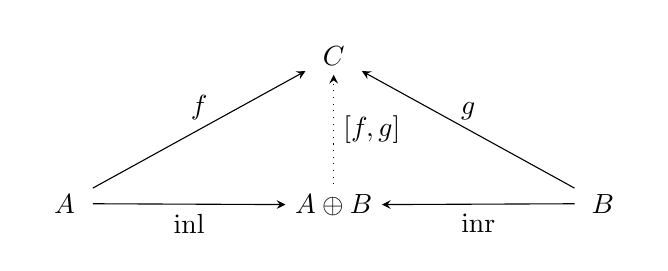
\begin{tikzpicture}
  \matrix (m) [matrix of math nodes,row sep=4em,column sep=7em,minimum width=2em]
  {
   & C &  \\
    A  & A \oplus B & B\\
  };
  \path[-stealth]
    (m-2-1) edge  node [above] {$f$} (m-1-2)
    (m-2-3) edge  node [above] {$g$} (m-1-2)
    (m-2-1) edge  node [below] {$\inl$} (m-2-2)
    (m-2-3) edge  node [below] {$\inr$} (m-2-2)
    (m-2-2) edge [dotted]  node [right] {$[f,g]$} (m-1-2);
    ;
\end{tikzpicture}
\]
\end{definition}

\begin{definition}
        A monoidal category $\catC$ with coproducts is called
        distributive if for every object $A$ in $\catC$ the
        functor $- \otimes A$ preserves coproducts. Explicitly
        this means that the morphism,
        \[
                [\inl \otimes \id, \inr \otimes \id] : B \otimes A \oplus C \otimes                     A \to (B \oplus C) \otimes A
        \]
        is actually an isomorphism. We will denote the respective inverse
        by $\dist$. Note that if $\catC$ is monoidal closed then it is automatically
        distributive as left adjoints preserve all colimits.
\end{definition}

% Let $\mathcal{C}$ be a monoidal closed category and let $X,$ $Y,$ and $Z$ be objects in $\mathcal{C}$. The morphism $\dist_{X, Y,Z}: X \otimes  \left(Y \oplus Z\right) \xrightarrow{} \left(X \otimes Y\right) \oplus \left(X \otimes Y\right)$, denotes the distributive property of the tensor product over the coproduct.  This distributive property holds in monoidal closed categories with coproducts because the tensor functor is a left adjoint (to the internal hom), and left adjoints preserve colimits.

Before presenting the interpretation of $\lambda$-calculus with conditionals in
distributive symmetric monoidal (closed) categories let us give some examples
of the latter in order to illustrate our work's broad range of applicability.

\begin{example}
Examples of monoidal closed categories with coproducts include the category of sets, the category of vector spaces, and the category of partial orders. In the category of sets, the tensor product is the cartesian product, the monoidal unit is the singleton set, the coproduct is the disjoint union, and the internal hom consists of all functions between sets. For the category of vector spaces, the tensor product is the standard tensor product of vector spaces, the monoidal unit is the field of scalars, the coproduct is the direct sum, and the internal hom is the space of linear maps. In the category of partial orders, the tensor product corresponds to the meet ($\wedge$), the monoidal unit to the the singleton poset, the coproduct to the join ($\vee$), and the internal hom is the poset of monotone functions ordered pointwise.
\end{example}

We now present the interpretation of $\lambda$-calculus with conditionals.
First the new type $A \oplus B$ is interpreted as $\sem{A \oplus B} = [\![A
]\!] \oplus [\![ B ]\!]$. As for the new terms, the corresponding
interpretation is defined inductively in \autoref{fig:denotational_sem cond}.

\begin{figure}[H]
  \begin{equation*}
  \begin{aligned}
  &\hspace{10pt}
  %
  \begin{prooftree}
      \hypo{ [\![\Gamma \vljud v: \typeA]\!] = m }
      \infer1[]{ [\![ \Gamma \vljud \text{inl}_{\typeB} (v):  \typeA \oplus \typeB  ]\!] = \inl  \comp m}
  \end{prooftree}
  %
  \hspace{120pt}
  %
  \begin{prooftree}
    \hypo{ [\![\Gamma \vljud v: \typeB]\!] = m }
    \infer1[]{ [\![ \Gamma \vljud \text{inr}_{\typeA} (v):  \typeA \oplus \typeB  ]\!] = \inr  \comp m}
\end{prooftree}
  %
  \\[20pt]
  &\hspace{-20pt}
  %
  \begin{prooftree}
      \hypo{[\![\Gamma\vljud v: \typeA \oplus \typeB ]\!] = b}
      \hypo{[\![\Delta, x:\typeA \vljud w: \typeD ]\!] = p}
      \hypo{ [\![\Delta,y:\typeB \vljud u: \typeD ]\!] = q }
      \hypo{E \in \Shuff(\Gamma; \Delta)}
      \infer4[]{ [\![E \vljud \text{case } v\,  \{\text{inl}_{\typeB} (x) \Rightarrow w ;\, \text{inr}_{\typeA} (y) \Rightarrow u\}: \typeD ]\!] =   [p,q] \comp (\text{jn}_{\Delta;\typeA}\comp \sw \oplus \text{jn}_{\Delta;\typeB}\comp \sw) \comp \dist \comp (b \otimes \text{id}) \comp \text{sp}_{\Gamma;\Delta} \comp \text{sh}_{E}}
  \end{prooftree}
  %
  \\[10pt]
  \end{aligned}
  \end{equation*}
  \caption{Judgment interpretation for conditionals}
\label{fig:denotational_sem cond}
\end{figure}


The next step is to demonstrate that the equations in Figure \ref{fig:equations-in-context-cond} are valid under the given interpretation. To achieve this, we first establish the following lemma.

\begin{lemma}[Exchange and Substitution]
\label{lem_interpret_exch:sub} 
For all judgements $\Gamma,x:\typeA, y:\typeB, \Delta \vljud v: \typeD, \> $
$\Gamma,x:\typeA \vljud v: \typeB$ and $\Delta \vljud w: \typeA$  the following
equations hold: 
  \begin{equation*}
\begin{split}
  [\![\Gamma,x:\typeA, y:\typeB, \Delta \vljud v: \typeD]\!] = [\![\Gamma,y:\typeB,x:\typeA,  \Delta \vljud v: \typeD]\! ] \comp \text{exch}_{\Gamma, \underline{ \typeA, \typeB} ,\Delta} \\
  [\![\Gamma, \Delta \vljud v[w/x]: \typeB]\!] = [\![\Gamma, x:\typeA \vljud v: \typeB]\!]\comp \text{jn}_{\Gamma;\typeA} \comp (\text{id} \otimes [\![ \Delta  \vljud w: \typeA]\!] ) \comp \text{sp}_{\Gamma;\Delta} 
\end{split}
  \end{equation*}
\end{lemma}

\begin{proof}
  We begin with the exchange property. The rules involving injections are
  straightforward. As for the rule~$\rulename{case}$, we distinguish between
  the scenarios where both variables ($x : \typeA$ and $y : \typeB$) are in
  $\Gamma$, both are in $\Delta$, or they are distributed across $\Gamma$ and
  $\Delta$. We begin with the first case. 
  \begin{align*}
    & \sem{\Gamma,x, y, \Delta \vljud \text{case }  v\,  \{\text{inl}_{\typeD} (a) \Rightarrow w ;\, \text{inr}_{\typeE} (b) \Rightarrow u\}} \\ 
    &\triangleq   [\sem{w}  , \sem{u}] \comp (\text{jn}_{E;\typeD}
    \comp \sw \oplus \text{jn}_{E;\typeE } \comp \sw) 
    \comp (\sem{ v} \otimes \id)  
    \comp \text{sp}_{\Gamma_{1},\typeA, \typeB,\Gamma_{2};E} 
    \comp \text{sh}_{\Gamma,\typeA, \typeB,\Delta}
    & \\
    & =  [\sem{w},\sem{u}] \comp (\text{jn}_{E;\typeD}
    \comp \sw \oplus \text{jn}_{E;\typeE } \comp \sw) 
    \comp (\sem{v} \comp\, \text{exch}_{\Gamma_{1}, \underline{\typeA,\typeB},\Gamma_{2}} 
    \otimes \id) \comp \text{sp}_{\Gamma_{1},\typeA, \typeB,\Gamma_{2};E} 
    \comp \text{sh}_{\Gamma,\typeA, \typeB,\Delta}
    & \text{(Induction)}\\
    &  =  \dots  \comp (\sem{v} \otimes \id) 
          \comp (\text{exch}_{\Gamma_1, \underline{\typeA, \typeB}, \Gamma_2} \otimes \text{id}) \comp \text{sp}_{\Gamma_{1},\typeA,\typeB, \Gamma_{2};E} \comp  \text{sh}_{\Gamma,\typeA, \typeB,\Delta} & {}\\
    & = \dots \comp (\sem{v} \otimes \id) \comp \text{sp}_{\Gamma_{1},\typeB,\typeA, \Gamma_{2};E} 
          \comp \text{sh}_{\Gamma,\typeB, \typeA,\Delta}  
          \comp \text{exch}_{\Gamma,  \underline{\typeA,\typeB}, \Delta} 
    & {\text{(Coherence)}} \\
    & \triangleq \sem{\Gamma,y, x, \Delta \vljud \text{case } v\,  \{\text{inl}_{\typeE} (a) \Rightarrow w ;\, \text{inr}_{\typeD} (b) \Rightarrow u\}} 
    \comp \text{exch}_{\Gamma,  \underline{\typeA, \typeB}, \Delta}
  \end{align*}
Let us now focus on the second case, \ie\ both variables live in $\Delta$.
%
%The second case follows by induction, the coherence theorem for symmetric monoidal categories, the universal property of the coproduct, and naturality of $\alpha,$ $\lambda,$ $\rho,$ and $\sw$ and their inverses.
%
% \left[[\![ w ]\!] ,[\![ u ]\!]\right] \comp (\text{jn}_{\Delta_{1},\typeA,\typeB}\comp \sw \oplus \text{jn}_{\Delta_{1},\typeA,\typeB} \comp \sw 
\begin{align*}
  & \sem{\Gamma,x, y, \Delta \vljud \text{case } \, v\, \{\text{inl} (a) \Rightarrow w ;\, \text{inr} (b) \Rightarrow u\}} \\
  & \triangleq  [\sem{w} ,\sem{u}]\comp (\text{jn}
  \comp \sw \oplus \text{jn} \comp \sw) 
  \comp \dist \comp (\sem{v} \otimes \id) \comp 
  \text{sp}_{} 
  \comp \text{sh}_{}  \\
  & = [\sem{ w }  \comp \text{exch}, \sem{u}\comp \text{exch}] \comp (\text{jn}\comp \sw \oplus \text{jn} \comp \sw) \comp \dist \comp (\sem{v} \otimes \id) \comp\text{sp} \comp \text{sh}
  & \text{(Induction)}\\
  & = [\sem{ w }, \sem{u}] 
  \comp (\text{exch} \oplus \text{exch}) 
  \comp (\text{jn}\comp \sw \oplus \text{jn} \comp \sw) 
  \comp \dist \comp (\sem{v} \otimes \id) \comp\text{sp} \comp \text{sh} 
  & \text{(Coproduct laws)}
  \\
  & = [\sem{ w }, \sem{u}] 
  \comp (\text{jn}\comp \sw \oplus \text{jn} \comp \sw) 
  \comp (\id \otimes \text{exch} \oplus \id \otimes \text{exch})
  \comp \dist \comp (\sem{v} \otimes \id) \comp\text{sp} \comp \text{sh} 
  & \text{(Coherence)}
  \\
  & = [\sem{ w }, \sem{u}] 
  \comp (\text{jn}\comp \sw \oplus \text{jn} \comp \sw) 
  \comp \dist 
  \comp (\id \otimes \text{exch}) \comp (\sem{v} \otimes \id) \comp\text{sp} \comp \text{sh} 
  & \text{(Naturality)}
  \\
  & = [\sem{ w }, \sem{u}] 
  \comp (\text{jn}\comp \sw \oplus \text{jn} \comp \sw) 
  \comp \dist 
  \comp (\sem{v} \otimes \id) \comp\text{sp} \comp \text{sh} 
  \comp \text{exch}
  & \text{(Coherence)}
  \\
  & \triangleq \sem{\Gamma,y, x, \Delta \vljud \text{case } v\,  \{\text{inl} (a) \Rightarrow w ;\, \text{inr} (b) \Rightarrow u\}} 
  \comp \text{exch}_{}
  %& = [[\![ w ]\!] \comp \text{jn}_{\Delta_{1} ,\typeB,\typeA,  \Delta_{2};\typeD} \comp \text{sp}_{\Delta_{1}, \typeB, \typeA, \Delta_{2};\typeD} \comp  \text{exch}_{\Delta_{1},\underline{\typeA,\typeB},  \Delta_{2},\typeD} \comp  \text{jn}_{\Delta_{1},\typeA,\typeB,  \Delta_{2};\typeD}  ,    [\![u ]\!] \comp \text{jn}_{\Delta_{1} ,\typeB,\typeA,  \Delta_{2};\typeE} & {\text{(coherence)}} \\
  %& \hspace{10pt} \comp \text{sp}_{\Delta_{1}, \typeB, \typeA, \Delta_{2};\typeE} \comp  \text{exch}_{\Delta_{1},\underline{\typeA,\typeB},  \Delta_{2},\typeE} \comp  \text{jn}_{\Delta_{1},\typeA,\typeB,  \Delta_{2};\typeE} ] \comp \dist \comp \sw \comp ([\![  v : \typeD \oplus \typeE  ]\!] \otimes \text{id}) \\
  %& \hspace{10pt} \comp\text{sp}_{E; \Delta_{1},\typeA,\typeB,  \Delta_{2}} \comp \text{sh}_{\Gamma,\typeA, \typeB,\Delta} \\
%  & = [[\![ w ]\!] ,  [\![u ]\!]] \comp  (\text{jn}_{\Delta_{1},\typeA,\typeB,  \Delta_{2};\typeD} \comp \sw \oplus \text{jn}_{\Delta_{1},\typeA,\typeB,  \Delta_{2};\typeE} \comp \sw ) \comp (\text{sp}_{\typeD;\Delta_{1}, \typeB, \typeA, \Delta_{2}} \comp  \text{exch}_{\typeD, \Delta_{1},\underline{\typeA,\typeB},  \Delta_{2}}   & {\text{(coherence and}} \\
%  & \hspace{10pt} \comp \text{jn}_{\typeD;\Delta_{1},\typeA,\typeB,  \Delta_{2}} \oplus \text{sp}_{\typeE;\Delta_{1}, \typeB, \typeA, \Delta_{2}} \comp  \text{exch}_{\typeE, \Delta_{1},\underline{\typeA,\typeB},  \Delta_{2}} \comp \text{jn}_{\typeE;\Delta_{1},\typeA,\typeB,  \Delta_{2}} )   \comp \dist \comp \sw \comp ([\![  v : \typeD \oplus \typeE  ]\!] & {\text{law of coproducts)}}  \\
%  & \hspace{10pt} \otimes \text{id})  \comp\text{sp}_{E; \Delta_{1},\typeA,\typeB,  \Delta_{2}} \comp \text{sh}_{\Gamma,\typeA, \typeB,\Delta} \\ 
\end{align*}
%The commutativity of the following diagram follows from the universal property of the coproduct and the naturality of $\alpha,$ $\lambda,$ $\rho,$ and $\sw$, their inverses, and their composition. Here $\phi$ corresponds to $\text{sp}_{\typeD \oplus \typeE;\Delta_{1}, \typeB, \typeA, \Delta_{2}} \comp  \text{exch}_{\typeD \oplus \typeE, \Delta_{1},\underline{\typeA,\typeB},  \Delta_{2}} \comp \text{jn}_{\typeD \oplus \typeE;\Delta_{1},\typeA,\typeB,  \Delta_{2}}$, $\phi_1$ to $\text{sp}_{\typeD;\Delta_{1}, \typeB, \typeA, \Delta_{2}} \comp  \text{exch}_{\typeD, \Delta_{1},\underline{\typeA,\typeB},  \Delta_{2}} \comp \text{jn}_{\typeE;\Delta_{1},\typeA,\typeB,  \Delta_{2}}$, and $\phi_2$ to $\text{sp}_{\typeE;\Delta_{1}, \typeB, \typeA, \Delta_{2}} \comp  \text{exch}_{\typeE, \Delta_{1},\underline{\typeA,\typeB},  \Delta_{2}} \comp \text{jn}_{\typeE;\Delta_{1},\typeA,\typeB,  \Delta_{2}}$.

%\hspace{-12pt} 
%\begin{tikzpicture} 
%  \matrix (m) [matrix of math nodes,row sep=4em,column sep=6em,minimum width=1em]
%  {
%    ([\![\typeD ]\!]\oplus [\![\typeE]\!]) \otimes \left([\![ \Delta_{1},\typeA,\typeB, \Delta_{2} ]\!]\right)   & ([\![\typeD ]\!]\oplus [\![\typeE]\!]) \otimes  \left([\![ \Delta_{1},\typeB,\typeA, \Delta_{2} ]\!]\right)      \\
%    \left(  [\![\typeD ]\!] \otimes [\![ \Delta_{1},\typeA,\typeB, \Delta_{2} ]\!]  \right) \oplus \left( [\![\typeE ]\!] \otimes [\![ \Delta_{1},\typeA,\typeB, \Delta_{2} ]\!]  \right)  &  \left( [\![\typeD ]\!] \otimes [\![ \Delta_{1},\typeB,\typeA, \Delta_{2} ]\!] \right) \oplus \left([\![\typeE ]\!] \otimes [\![ \Delta_{1},\typeB,\typeA, \Delta_{2} ]\!] \right) \\
%  };
%  \path[-stealth]
%    (m-1-1) edge node [above] {$ \phi$} (m-1-2)
%    (m-2-1)  edge[bend right=-10] node [pos=0.5, shift={(-1.4, 0)}] {$[\inl \otimes \text{id}, \inr \otimes\text{id}]$} (m-1-1)
%    (m-1-1) edge [bend left=10] node [pos=0.5, shift={(0.4,0)}] {$\dist$} (m-2-1)
%    (m-2-1) edge node [above] {$ \phi_1 \oplus \phi_2 $} (m-2-2)
%    (m-1-2) edge [bend left=10] node [pos=0.5, shift={(0.4,0)}] {$\dist$} (m-2-2)
%    (m-2-2)  edge[bend right=-10] node [pos=0.5, shift={(-1.4, 0)}] {$[\inl \otimes \text{id},\inr \otimes \text{id}]$} (m-1-2)
%    ;
%\end{tikzpicture}
%
%The commutativity of the diagram is established as follows:
%\begin{align*}
%  & [\inl \otimes \text{id},\inr \otimes \text{id}] \comp (\phi_1 \oplus \phi_2)\\  
%  & = [\inl \otimes \text{id},\inr \otimes \text{id}] \comp [\inl \comp \phi_1,\inr \comp \phi_2 ] \\
%  & = [(\inl \otimes \text{id}) \comp \phi_1,(\inr \otimes \text{id}) \comp \phi_2 ] & {\text{(law of coproducts)}}  \\
%  & = [\phi \comp (\inl \otimes \text{id}), \phi \comp (\inr \otimes \text{id})] & {\text{(naturality)}} \\
%  & = \phi \comp  [\inl \otimes \text{id},\inr \otimes \text{id}]  & {\text{(law of coproducts)}}
%\end{align*}
 
%As a result it holds that 
%\begin{align*}
%  & [[\![ w ]\!] ,  [\![u ]\!]] \comp  (\text{jn}_{\Delta_{1},\typeA,\typeB,  \Delta_{2};\typeD} \comp \sw \oplus \text{jn}_{\Delta_{1},\typeA,\typeB,  \Delta_{2};\typeE} \comp \sw ) \comp (\text{sp}_{\typeD;\Delta_{1}, \typeB, \typeA, \Delta_{2}} \comp  \text{exch}_{\typeD, \Delta_{1},\underline{\typeA,\typeB},  \Delta_{2}}   \\
%  & \hspace{10pt} \comp \text{jn}_{\typeD;\Delta_{1},\typeA,\typeB,  \Delta_{2}} \oplus \text{sp}_{\typeE;\Delta_{1}, \typeB, \typeA, \Delta_{2}} \comp  \text{exch}_{\typeE, \Delta_{1},\underline{\typeA,\typeB},  \Delta_{2}} \comp \text{jn}_{\typeE;\Delta_{1},\typeA,\typeB,  \Delta_{2}} )   \comp \dist \comp \sw \comp ([\![  v : \typeD \oplus \typeE  ]\!]  \\
%  & \hspace{10pt} \otimes \text{id})  \comp\text{sp}_{E; \Delta_{1},\typeA,\typeB,  \Delta_{2}} \comp \text{sh}_{\Gamma,\typeA, \typeB,\Delta} \\
%  & = [[\![ w ]\!] ,  [\![u ]\!]] \comp  (\text{jn}_{\Delta_{1},\typeA,\typeB,  \Delta_{2};\typeD} \comp \sw \oplus \text{jn}_{\Delta_{1},\typeA,\typeB,  \Delta_{2};\typeE} \comp \sw ) \comp \dist \comp \text{sp}_{\typeD \oplus \typeE;\Delta_{1}, \typeB, \typeA, \Delta_{2}} \comp  \text{exch}_{\typeD \oplus \typeE, \Delta_{1},\underline{\typeA,\typeB},  \Delta_{2}} \\
%  & \hspace{10pt} \comp \text{jn}_{\typeD \oplus \typeE;\Delta_{1},\typeA,\typeB,  \Delta_{2}} \comp ([\![  v ]\!] \otimes \text{id})  \comp\text{sp}_{E; \Delta_{1},\typeA,\typeB,  \Delta_{2}} \comp \text{sh}_{\Gamma,\typeA, \typeB,\Delta}\\
%  & = [[\![ w ]\!] ,  [\![u ]\!]] \comp  (\text{jn}_{\Delta_{1},\typeA,\typeB,  \Delta_{2};\typeD} \comp \sw \oplus \text{jn}_{\Delta_{1},\typeA,\typeB,  \Delta_{2};\typeE} \comp \sw ) \comp \dist  \comp ([\![  v  ]\!] \otimes \text{id}) \comp \text{sp}_{E;\Delta_{1}, \typeB, \typeA, \Delta_{2}} & {\text{(naturality)}} \\
%  & \hspace{10pt}  \comp  \text{exch}_{E, \Delta_{1},\underline{\typeA,\typeB},  \Delta_{2}} \comp  \text{jn}_{E ;\Delta_{1},\typeA,\typeB,  \Delta_{2}}   \comp\text{sp}_{E; \Delta_{1},\typeA,\typeB,  \Delta_{2}} \comp \text{sh}_{\Gamma,\typeA, \typeB,\Delta} \\
%  & = [[\![ w ]\!] ,  [\![u ]\!]] \comp  (\text{jn}_{\Delta_{1},\typeA,\typeB,  \Delta_{2};\typeD} \comp \sw \oplus \text{jn}_{\Delta_{1},\typeA,\typeB,  \Delta_{2};\typeE} \comp \sw ) \comp \dist  \comp ([\![  v  ]\!] \otimes \text{id}) \comp \text{sp}_{E; \Delta_{1}, \typeB,\typeA,  \Delta_{2}} & {\text{(coherence)}} \\
%  & \hspace{10pt} \comp  \text{sh}_{\Gamma; \typeB,\typeA, \Delta} \comp  \text{exch}_{E, \Delta_{1},\underline{\typeA,\typeB},  \Delta_{2}} \\
%  & \triangleq [\![\Gamma,y:\typeB, x:\typeA, \Delta \vljud \text{case } \,  \{\text{inl}_{\typeD} (a) \Rightarrow w ;\, \text{inr}_{\typeE} (b) \Rightarrow u\}: \typeF]\!] \comp \text{exch}_{\Gamma,\underline{\typeA,  \typeB}, \Delta}
%\end{align*}
%

The proof the for the third case follows directly from the coherence theorem
for symmetric monoidal categories.

Regarding the substitution rule, once again the cases involving the injections follow directly by induction on the derivation tree. For the rule (case), we distinguish between the scenarios where the variable $x$ is in $\Gamma$ or in $\Delta$. The first case follows from induction, the bifunctoriality of the tensor product, and the naturality of $\alpha$, $\lambda$, $\rho$, $\sw$, their inverses, and their respective compositions.

% \left[[\![ w ]\!] ,[\![ u ]\!]\right] \comp (\text{jn}_{\Delta;\typeD}\comp \sw \oplus \text{jn}_{\Delta;\typeE } \comp \sw)
\begin{align*}
  &[\![E, Z \vljud \text{case } v \,  \{\text{inl} (a) \Rightarrow w ;\, \text{inr} (b) \Rightarrow u\} [t/x]]\!] \\
  & \triangleq \left[[\![ w ]\!] ,[\![ u ]\!]\right] \comp (\text{jn}\comp \sw \oplus \text{jn} \comp \sw) \comp \dist \comp  ([\![ v [t/x] ]\!]   \otimes \text{id})  \comp \text{sp} \comp \text{sh} \\
  & = \left[[\![ w ]\!] ,[\![ u ]\!]\right] \comp (\text{jn} \comp \sw \oplus \text{jn} \comp \sw)  \comp \dist \comp (([\![ v]\!]  \comp \text{jn} \comp (\text{id} \otimes [\![  t ]\!] ) \comp \text{sp} )\otimes \text{id})  \comp \text{sp} \comp \text{sh} & {\text{(Induction)}} \\
  & =  \left[[\![ w ]\!] ,[\![ u ]\!]\right] \comp (\text{jn} \comp \sw \oplus \text{jn} \comp \sw)  \comp \dist  \comp ([\![ v]\!] \otimes \text{id}) \comp (\text{jn} \comp (\text{id} \otimes [\![  t ]\!] ) \comp \text{sp} \otimes \text{id})  \comp \text{sp}\comp \text{sh}\\
  & = \left[[\![ w ]\!] ,[\![ u ]\!]\right] \comp (\text{jn} \comp \sw \oplus \text{jn} \comp \sw)  \comp \dist  \comp ([\![ v]\!] \otimes \text{id})  \comp (\text{jn} \comp (\text{id} \otimes [\![  t ]\!] ) \comp \text{sp} \otimes \text{id})  \comp \text{sp} \comp \text{sh} \comp \text{jn} \comp \text{sp} & {(\text{Coherence})} \\
  & = \left[[\![ w ]\!] ,[\![ u ]\!]\right] \comp (\text{jn} \comp \sw \oplus \text{jn} \comp \sw)  \comp \dist  \comp ([\![ v]\!] \otimes \text{id}) \comp (\text{jn}\comp \text{sp} \otimes   \id) \comp \text{sp}   \comp \text{sh} \comp \text{jn}\comp (\text{id} \otimes [\![ t ]\!] ) \comp \text{sp}  & {(\text{Naturality})}   \\
  & = \left[[\![ w ]\!] ,[\![ u ]\!]\right] \comp (\text{jn} \comp \sw \oplus \text{jn}\comp \sw)  \comp \dist  \comp ([\![ v]\!] \otimes \text{id}) \comp \text{sp}  \comp \text{sh}  \comp  \text{jn} \comp (\text{id} \otimes [\![ t ]\!] ) \comp \text{sp}  & {(\text{Coherence})}   \\
  & \triangleq \, [\![E,  x \vljud \text{case } v\,  \{\text{inl} (x) \Rightarrow w ;\, \text{inr} (y) \Rightarrow u\}]\!]  \comp  \text{jn} \comp (\text{id} \otimes [\![ t ]\!] ) \comp \text{sp}
\end{align*}


The second case follows from induction, the exchange rule, the universal property of the coproduct,  the bifunctoriality of the tensor product, and the naturality of $\alpha$, $\lambda$, $\rho$, and $\sw$, along with their inverses and respective compositions.

%\left[[\![ w ]\!] ,[\![ u ]\!]\right] \comp (\text{jn}_{\Delta;\typeD}\comp \sw \oplus \text{jn}_{\Delta;\typeE } \comp \sw)  \comp \dist
%\left[[\![ \Delta  , Z ,  a:\typeD \vljud w[t/x] ]\!] \comp \text{jn}_{ \Delta;\typeD},[\![ \Delta, Z, b:\typeE \vljud u[t/x]  ]\!] \comp \text{jn}_{ \Delta;\typeE}\right]
 
%\left[[\![ \Delta  , Z ,  a:\typeD \vljud w[t/x] ]\!] ,[\![ \Delta, Z, b:\typeE \vljud u[t/x]  ]\!] \right] \comp (\text{jn}_{ \Delta;\typeD} \comp \sw \oplus \text{jn}_{ \Delta;\typeE} \comp \sw)

\begin{align*}
  &[\![E, Z \vljud \text{case } v \,  \{\text{inl} (a) \Rightarrow w ;\, \text{inr} (b) \Rightarrow u\} [t/x]]\!] \\
  & \triangleq \left[[\![ \Delta  , Z ,  a:\typeD \vljud w[t/x] ]\!] ,[\![ \Delta, Z, b:\typeE \vljud u[t/x]  ]\!] \right] \comp (\text{jn}\comp \sw \oplus \text{jn} \comp \sw) \comp \dist  \comp ([\![ v ]\!]   \otimes \text{id})    \comp \text{sp} \comp \text{sh} \hspace{10pt} \\
  & =  \left[[\![ \Delta  ,   a:\typeD, Z \vljud w[t/x] ]\!] ,[\![ \Delta, b:\typeE, Z \vljud u[t/x]  ]\!] \right] \comp ( \text{exch}_{\Delta,Z,\typeD} \comp \text{jn}\comp \sw \oplus  \text{exch} \comp \text{jn} \comp \sw)   \comp \dist   & {(\text{Exchange and}} \\
  &  \hspace{10pt} \comp \sw  \comp ([\![v]\!] \otimes \text{id})  \comp \text{sp} \comp \text{sh} & { \text{coproduct laws})}   \\
  & =   \left[[\![w ]\!] ,[\![ u]\!] \right] \comp ( \text{jn} \comp (\text{id} \otimes [\![t]\!] ) \comp \text{sp} \comp  \text{exch} \comp \text{jn} \comp \sw  \oplus  \text{jn} \comp (\text{id} \otimes [\![ t]\!] ) \comp \text{sp}  \comp \text{exch} \comp\text{jn} \comp \sw ) \comp \dist & {\text{(Induction)}}  \\
  & \hspace{10pt}     \comp ([\![v]\!] \otimes \text{id})  \comp \text{sp} \comp \text{sh} \\
  & =  \left[[\![w ]\!] ,[\![ u]\!] \right] \comp (\text{exch} \comp \text{jn} \comp \sw \comp (\text{id} \otimes  \text{jn} ) \comp (\text{id} \otimes [\![t]\!]) \comp  (\text{id} \otimes \text{sp} ) \oplus \text{exch} \comp \text{jn} \comp \sw \comp (\text{id} \otimes  \text{jn} )   & {(\text{Naturality and }} \\
  & \hspace{10pt} \comp (\text{id} \otimes [\![t]\!]) \comp  (\text{id} \otimes \text{sp} ) )\comp \dist \comp ([\![v]\!] \otimes \text{id})  \comp \text{sp} \comp \text{sh} & {\text{coproduct laws})} \\
  & =  \left[[\![w]\!] ,[\![u]\!] \right] \comp (\text{exch} \comp \text{jn} \comp \sw \comp (\text{id} \otimes  (\text{jn} \comp \text{id} \otimes [\![t]\!] \comp \text{sp}) ) \oplus  \text{exch} \comp \text{jn} \comp \sw  &  \\
  & \hspace{10pt}  \comp (\text{id} \otimes  (\text{jn}\comp \text{id} \otimes [\![t]\!] \comp \text{sp}) ))\comp \dist \comp ([\![v]\!] \otimes \text{id}) \comp \text{sp}\comp \text{sh}  \\
  & = [[\![ \Delta  , x:\typeA ,  a:\typeD \vljud w]\!] , [\![ \Delta  , x:\typeA ,  b:\typeE \vljud u]\!]]  \comp (  \text{jn} \comp \sw \comp (\text{id} \otimes  (\text{jn} \comp \id \otimes [\![t]\!]  \comp \text{sp})  \oplus \text{jn} \comp  \sw      & {(\text{Exchange and }}  \\
  & \hspace{10pt} \comp (\text{id} \otimes  (\text{jn} \comp \text{id} \otimes [\![t]\!] \comp \text{sp}) )  ) \comp \dist \comp ([\![v]\!] \otimes \text{id})   \comp \text{sp}\comp \text{sh}  & { \text{coproduct laws})}\\
  &= \left[[\![w ]\!] ,[\![ u]\!] \right] \comp  (\text{jn} \comp \sw \oplus \text{jn} \comp \sw)  \comp \dist \comp ( \text{id} \otimes (\text{jn} \cdot (\text{id} \otimes [\![t]\!]) \cdot \text{sp} ) ) \comp ([\![v]\!] \otimes \text{id}) \comp \text{sp} \comp \text{sh} & {(\text{Coproduct laws}}  \\
  & & {\text{and naturality}}) \\
  & =  \left[[\![w ]\!] ,[\![ u]\!] \right] \comp  (\text{jn} \comp \sw \oplus \text{jn}\comp \sw)  \comp \dist \comp  ([\![v]\!] \otimes \text{id}) \comp \text{sp} \comp ( \text{id} \otimes (\text{jn} \comp  (\text{id} \otimes [\![t]\!]) \cdot \text{sp} ) ) \comp \text{sp}\comp \text{sh}     & {(\text{Coherence})} \\
  &  \hspace{10pt}  \comp \text{jn}  \comp \text{sp} & \\
  & = \left[[\![w ]\!] ,[\![ u]\!] \right] \comp  (\text{jn} \comp \sw \oplus \text{jn} \comp \sw)  \comp \dist \comp  ([\![v]\!] \otimes \text{id})  \comp ( \id \otimes \text{jn} \comp \text{sp}) \comp \text{sp}  \comp \text{sh}    \comp \text{jn} \comp (\text{id} \otimes [\![ t ]\!] ) \comp \text{sp} & {(\text{Naturality})}   \\
  & =  [[\![w]\!], [\![u]\!]] \comp (\text{jn} \comp \sw \oplus \text{jn} \comp \sw)  \comp \dist   \comp ([\![v  ]\!] \otimes \text{id}) \comp \text{sp} \comp \text{sh} \comp \text{jn} \comp (\text{id} \otimes [\![ t ]\!] ) \comp \text{sp}  & {(\text{Coherence})}     \\ 
  & \triangleq  [\![E,  x\vljud \text{case } v\,  \{\text{inl} (a) \Rightarrow w ;\, \text{inr} (b) \Rightarrow u\}]\!] \comp \text{jn} \comp (\text{id} \otimes [\![ t ]\!] ) \comp \text{sp}
\end{align*}
\end{proof}

\begin{theorem} \label {theorem:eq_in_context}
  The equations presented in Figure \ref{fig:equations-in-context-cond} are sound w.r.t. judgement interpretation. More specifically if $ \Gamma \vljud v = w: \typeA$ is one of the equations in Figure \ref{fig:equations-in-context-cond} then $[\![ \Gamma \vljud v: \typeA ]\!] = [\![ \Gamma \vljud w: \typeA ]\!]$.
\end{theorem}

%[\llbracket w\rrbracket,\llbracket u \rrbracket] \comp (\text{jn}_{\Delta;\typeA} \comp \sw \oplus \text{jn}_{\Delta;\typeB} \comp \sw  )

\begin{proof}
  Follows from Lemma \autoref{lem_interpret_exch:sub}, the coherence theorem for symmetric monoidal categories, naturality,  the bifunctoriality of the tensor product, and the universal property of the coproduct.   
  We will provide a complete proof for the first and third equations, noting that the proof for the second equation follows analogously from the first.
  \begin{align*}
    &\llbracket \Delta,\Gamma \vljud  \text{case }  \text{inl}(v)\, \{\text{inl} (x) \Rightarrow w ;\, \text{inr}_{\typeA} (y) \Rightarrow u\} \rrbracket \\
    & \triangleq  [\llbracket w\rrbracket,\llbracket u \rrbracket] \comp (\text{jn} \comp \sw \oplus \text{jn} \comp \sw  ) \comp \dist \comp \sw \comp (\inl \comp \llbracket  v \rrbracket \otimes \text{id}) \comp \text{sp} \comp \text{sh} \\
    & =  [\llbracket w\rrbracket,\llbracket u \rrbracket] \comp (\text{jn} \comp \sw \oplus \text{jn} \comp \sw ) \comp \dist \comp (\inl \otimes \text{id}  ) \comp ( \llbracket  v \rrbracket \otimes \text{id}) \comp \text{sp} \comp \text{sh}  \\
    & =  [\llbracket w\rrbracket,\llbracket u \rrbracket] \comp (\text{jn} \comp \sw \oplus \text{jn} \comp \sw ) \comp \dist \comp [\inl \otimes \id, \inr \otimes \id] \comp \inl  \comp ( \llbracket  v \rrbracket \otimes \text{id}) \comp \text{sp} \comp \text{sh}  &(\text{Coproduct laws})\\
    & =  [\llbracket w\rrbracket,\llbracket u \rrbracket] \comp (\text{jn} \comp \sw \oplus \text{jn} \comp \sw )  \comp \inl  \comp ( \llbracket  v \rrbracket \otimes \text{id}) \comp \text{sp} \comp \text{sh} \\
    & = \llbracket  w \rrbracket\comp \text{jn} \comp   \sw \comp(\llbracket v \rrbracket \otimes  \text{id}) \comp \text{sp} \comp \text{sh} & {\text{(Coproduct laws)}} \\
    &=  \llbracket  w \rrbracket\comp \text{jn} \comp(  \text{id}\otimes \llbracket v \rrbracket ) \comp   \sw \comp \text{sp} \comp \text{sh} & {\text{(Naturality)}} \\
    &= \llbracket w \rrbracket \comp \text{jn} \comp( \text{id} \otimes \llbracket v \rrbracket) \comp \text{sp} & {\text{(Coherence)}}\\
    & = \llbracket w[v/x]  \rrbracket  & {\text{(Lemma \ref{lem_interpret_exch:sub})}}
\end{align*}

%\todo[inline,size=\normalsize]{Elitzur‑Vaidman Bomb Testing Problem -> Improve usando o efeito Zeno? -> Acho que não tem ifs} 

%%[\llbracket  w [ \text{inl}_{\typeB}(y)/x] \rrbracket, \llbracket  w [ \text{inr}_{\typeA}(z)/x] \rrbracket] \comp (\text{jn}_{\Delta;\typeA} \comp \sw \oplus \text{jn}_{\Delta;\typeB} \comp \sw  ) \comp \dist \comp

Regarding the third equation, we have that
\begin{align*}
  & \llbracket \Delta,\Gamma \vljud \text{case } v\, \{\text{inl}_{\typeB} (y) \Rightarrow w [ \text{inl}_{\typeB}(y)/x] ;\, \text{inr}_{\typeA} (z) \Rightarrow w [ \text{inr}_{\typeA}(z)/x]\}: \typeD\rrbracket \\
  & \triangleq  [\llbracket  w [ \text{inl}_{\typeB}(y)/x] \rrbracket, \llbracket  w [ \text{inr}_{\typeA}(z)/x] \rrbracket] \comp (\text{jn}_{\Delta;\typeA} \comp \sw \oplus \text{jn} \comp \sw  ) \comp \dist \comp (\llbracket v\rrbracket \otimes \text{id}) \comp  \text{sp} \comp \text{sh} \\
  & = \llbracket w \rrbracket \comp [\text{jn} \comp (\text{id} \otimes\inl \comp  \llbracket y:\typeA \vljud y:\typeA  \rrbracket) \comp \text{sp} \comp \text{jn} \comp \sw , 
   \text{jn}\comp (\text{id} \otimes\inr  \comp \llbracket z:\typeB \vljud z:\typeB  \rrbracket)   & {\text{(Lemma \ref{lem_interpret_exch:sub} and}} \\
  &  \hspace{10pt}\comp \text{sp} \comp \text{jn} \comp \sw  ] \comp \dist \comp (\llbracket v\rrbracket \otimes \text{id}) \comp  \text{sp} \comp \text{sh} & {\text{coproduct laws)}}  \\
  & =  \llbracket w \rrbracket \comp \text{jn} \comp [ (\text{id} \otimes\inl)  \comp \sw  ,     \comp (\text{id} \otimes\inr) \comp \sw  ] \comp \dist  \comp (\llbracket v \oplus \typeB\rrbracket \otimes \text{id})  \comp  \text{sp} \comp \text{sh}  & {\text{(Coherence and}}   \\
  & \hspace{10pt} & {\text{coproduct laws)}}   \\
  & = \llbracket w \rrbracket \comp \text{jn} \comp   \sw \comp  [\inl \otimes \text{id} , \inr \otimes \text{id}] \comp \dist   \comp (\llbracket v \oplus \typeB\rrbracket \otimes \text{id})  \comp  \text{sp}\comp \text{sh}  & {\text{(Naturality and}}  \\
  & \hspace{10pt} & {\text{coproduct laws})}   \\
  %& = \llbracket w \rrbracket \comp \text{jn}_{\Delta;\typeA \oplus \typeB} \comp \comp \sw \text{id}   \comp (\llbracket v \oplus \typeB\rrbracket \otimes \text{id})  \comp  \text{sp}_{\Gamma;\Delta} \comp \text{sh}_{\Delta;\Gamma}  \\
  & = \llbracket w \rrbracket \comp \text{jn} \comp ( \text{id} \otimes \llbracket v \oplus \typeB\rrbracket )  \comp  \sw  \comp  \text{sp} \comp \text{sh} & {\text{(Naturality)}}\\
  &  = \llbracket w \rrbracket \comp \text{jn} \comp ( \text{id} \otimes \llbracket v \oplus \typeB\rrbracket )  \comp  \text{sp} & {\text{(Coherence)}}\\
  & \triangleq \llbracket w[v/x] : \typeD \rrbracket & {\text{(Lemma \ref{lem_interpret_exch:sub})}}
\end{align*}
\end{proof}

\begin{definition}
  Consider a tuple $(G, \Sigma)$ consisting of a class $G$ of ground types and a class $\Sigma$ of sorted operation symbols. A \emph{linear} $\lambda$-\emph{theory} $((G, \Sigma), \textit{Ax})$ is a triple such that \emph{Ax} is a class of equations-in-context over linear $\lambda$-terms built from $(G, \Sigma)$.
\end{definition}

The elements of \emph{Ax} are called the axioms of the theory. Let \emph{Th(Ax)}  be the smallest congruence that contains \emph{Ax}, the equations-in-context, and that is closed under exchange
and substitution. We call the elements of  \emph{Th(Ax)} the \emph{theorems} of the theory.

\begin{definition}
  Consider a linear $\lambda$-theory $((\lambda, \Sigma), \emph{Ax})$ and
  also a distributive symmetric monoidal closed category  $\catC$. Suppose that for each $X \in G$ we have an interpretation $\llbracket X \rrbracket$
  that is a $\catC$-object and analogously for the operation symbols. This interpretation structure
  is a \emph{model} of the theory if all axioms are satisfied by the interpretation.
\end{definition}

\begin{theorem} \label {theorem:comp_eq_in_context}
  The equations presented in Figure \ref{fig:equations-in-context-cond} are complete w.r.t. judgment interpretation. More specifically, by combining these equations with the remaining equations from the linear lambda calculus, it becomes possible to derive the properties that must necessarily hold in every model.
\end{theorem}


\begin{proof}
  Completeness arises from constructing the syntactic category $\catSyn(\mathscr{T})$ of a $\lambda$-theory $\mathscr{T}$ (also known as term model). By employing the equations in Figure \ref{fig:equations-in-context-cond}, we show that both the universal property of the coproduct and the distributive property are satisfied in $\catSyn(\mathscr{T})$. The syntactic category of $\mathscr{T}$ has as objects the types of $\mathscr{T}$ and as morphisms $A \rightarrow B$ the equivalence classes (w.r.t. provability) of terms $v$ for which we can derive $x : \typeA \vljud v : \typeB$.

  In the syntactic category, the coproduct $[ p ,  q]$ can be seen as the equivalence
  class 
  $$\left[z:\typeA \oplus\typeB \vljud \text{case } z\,\{\inl_{\typeB}(x) \Rightarrow p ; \, \inr_{\typeA}(y) \Rightarrow q\}: \typeD\right],$$ 
  the distributive property, $\dist$, corresponds to the class 
  \begin{align*}
    \big[z:(\typeA \otimes \mathbb{\typeB}) \otimes \mathbb{\typeD} \vljud \text{pm } z \text{ to } a \otimes b. \text{ case } a\,\{ &\inl_{\typeB}(x) \Rightarrow \inl_{\typeB \otimes \typeD}(x \otimes b); \\
    & \inr_{\typeA}(y) \Rightarrow \inr_{\typeA \otimes \typeD} (y \otimes b)\}: (\typeA \otimes \typeD) \oplus (\typeB \otimes \typeD)\big],
  \end{align*}
and its inverse, $[\inl \otimes \id, \inr \otimes \id]$, to the class
\begin{align*}
  \big[z: (\typeA \otimes \typeD) \oplus (\typeB \otimes \typeD) \vljud  \text{ case } z \,\{ &\inl_{\typeB}(x) \Rightarrow \text{pm } x \text{ to } a \otimes b. \, \inl_{\typeB}(a) \otimes b; \\
  & \inr_{\typeA}(y) \Rightarrow \text{pm } y \text{ to } a' \otimes b'. \, \inr_{\typeA}(a') \otimes b'\}: (\typeA \otimes \mathbb{\typeB}) \otimes \mathbb{\typeD}\big].
\end{align*}


The proof of the coproduct diagram comutes follow directly from the $\beta$-equations in Figure \ref{fig:equations-in-context-cond}, $\alpha$-equivalence, and Lemma \ref{lem:exh_and_sub}. Specifically, for the left triangle in the coproduct diagram, we have that:
  \begin{align*}
    & \left[z:\typeA \oplus \typeB  \vljud \text{case } v\,\{\inl_{\typeB}(x) \Rightarrow p ; \, \inr_{\typeA}(y) \Rightarrow q\}: \typeD\right] \comp \left[ x: \typeA\vljud \inl_{\typeB}(x): \typeA \oplus \typeB \right]  \\
    =& \left(z:\typeA \oplus \typeB  \vljud \text{case } v\,\{\inl_{\typeB}(x) \Rightarrow p ; \, \inr_{\typeA}(y) \Rightarrow q\}: \typeD\right) \comp \left( x: \typeA\vljud \inl_{\typeB}(x): \typeA \oplus \typeB \right) 
   \\
    =& z:\typeA \oplus \typeB  \vljud \text{case } v\,\{\inl_{\typeB}(x') \Rightarrow p[x'/ x] ; \, \inr_{\typeA}(y) \Rightarrow q\}: \typeD \comp  x: \typeA\vljud \inl_{\typeB}(x): \typeA \oplus \typeB & (\alpha)\\
    = & x:\typeA \vljud \text{case } \inl(x) \,\{\inl_{\typeB}(x') \Rightarrow p[x'/ x] ; \, \inr_{\typeA}(y) \Rightarrow q\}: \typeD & (\text{Lemma } \ref{lem:exh_and_sub})  \\
    = &  x:\typeA \vljud p[x'/x][x/x']: \typeD & (\beta_{\text{case}}^{\text{inl}}) \\
    = & x:\typeA \vljud p: \typeD \\
    = &  \left[x:\typeA \vljud p: \typeD\right]  \\
  \end{align*}
  The proof for the right triangle in the coproduct diagram is analogous.
 
  Regarding the unicity of the coproduct, the key aspect of the proof lies in proving that the following equality holds: 
  $$\left[z:\typeA \oplus \typeB  \vljud \text{case } z \,\{\inl_{\typeB}(x) \Rightarrow m[\inl_{\typeB}(x)/ z] ; \, \inr_{\typeA}(y) \Rightarrow m[\inr_{\typeA}(x)/ z]\}: \typeD\right] = [z:\typeA \oplus \typeB \vljud m: \typeD].$$ 
  This equality follows direct from the $\eta$-equation in Figure \ref{fig:equations-in-context-cond}. Now, considering any morphism $m'$ from $\typeA \oplus \typeB$ to $\typeD$ and the coproduct diagram, we have that 
  %$$\left[z:\typeA \oplus \typeB  \vljud m': \typeD\right] \comp \left[ x: \typeA\vljud \inl_{\typeB}(x): \typeA \oplus \typeB \right] = \left[x: \typeA  \vljud p: \typeD\right]  $$ 
  $$\left[ x: \typeA \vljud m'[ \inl_{\typeB}(x)/z]: \typeD\right]  = \left[x: \typeA  \vljud p: \typeD\right]  $$ 
  and
  $$\left[ y: \typeB  \vljud m'[\inr_{\typeA}(y)/z]: \typeD\right] = \left[y: \typeB  \vljud q: \typeD\right].$$
  As a result, if follows from the equalities above that 
  \begin{align*}
    \left[z:\typeA \oplus \typeB  \vljud m': \typeD\right]& =\left[z:\typeA \oplus \typeB  \vljud \text{case } z \,\{\inl_{\typeB}(x) \Rightarrow m'[\inl_{\typeB}(x)/ z] ; \, \inr_{\typeA}(y) \Rightarrow m'[\inr_{\typeA}(x)/ z]\}: \typeD\right]\\
    & = \left[z:\typeA \oplus \typeB  \vljud \text{case } z \,\{\inl_{\typeB}(x) \Rightarrow p ; \, \inr_{\typeA}(y) \Rightarrow q\}: \typeD\right]. 
  \end{align*}
 
 
  To prove that the distributive property is an isomorphism syntactically, we first establish that the following equality, known  as the \emph{syntactic fusion law}, holds:
  \begin{equation*}
    \left[v\left[ \left(\text{case } a \,\{\inl_{\typeB}(x) \Rightarrow w ; \, \inr_{\typeA}(y) \Rightarrow u\}\right)  / z \right]\right] =   \left[\text{case } a \,\{\inl_{\typeB}(x) \Rightarrow v[w/z] ; \, \inr_{\typeA}(y) \Rightarrow v[u/z]\} \right].
  \end{equation*}
It should be noted that this equality corresponds semantically to the property  $ \llbracket v \rrbracket \comp [ \llbracket w \rrbracket,  \llbracket u \rrbracket] = [ \llbracket v \rrbracket \comp \llbracket w \rrbracket,\llbracket v \rrbracket \comp \llbracket u \rrbracket ] $.
This equality follows from the $\alpha$-equivalence and the equations in Figure \ref{fig:equations-in-context-cond}. 

\begin{align*}
  &\left[v\left[ \left(\text{case } a \,\{\inl_{\typeB}(x) \Rightarrow w ; \, \inr_{\typeA}(y) \Rightarrow u\}\right)  / z \right]\right] & \\
  &  = v \left[ \left(\text{case } a \,\{\inl_{\typeB}(x) \Rightarrow w ; \, \inr_{\typeA}(y) \Rightarrow u\}\right)  / z \right] & \\
  & =v  \left[ \left(\text{case } a \,\{\inl_{\typeB}(x') \Rightarrow w[x'/x] ; \, \inr_{\typeA}(y') \Rightarrow u[y'/y]\}\right)  / z \right] & (\alpha) \\
  & = \big[ \text{case } a \,\{\inl_{\typeB}(x) \Rightarrow v[\text{case } \inl_{\typeB}(x) \,\{\inl_{\typeB}(x') \Rightarrow w[x'/x] ; \, \inr_{\typeA}(y) \Rightarrow u[y'/y]\}/z] ; \, & (\eta_{\text{case}}) \ \\
   & \hspace{50pt} \inr_{\typeA}(y) \Rightarrow  v[\text{case } \inr_{\typeA}(y) \,\{\inl_{\typeB}(x') \Rightarrow w[x'/x] ; \, \inr_{\typeA}(y) \Rightarrow u[y'/y]\}/z]\}\big]  \\
   & = \text{case } a \,\{\inl_{\typeB}(x) \Rightarrow v[w[x'/x][x/x']/z] ; \, \inr_{\typeA}(y) \Rightarrow v[u[y'/y][y/y']/z]\}   & (\beta_{\text{case}}^{\text{inl}} \text{ and } \beta_{\text{case}}^{\text{inr}}  ) \\
   & =  \text{case } a \,\{\inl_{\typeB}(x) \Rightarrow v[w/z] ; \, \inr_{\typeA}(y) \Rightarrow v[u/z]\}  \\
   & = \left[ \text{case } a \,\{\inl_{\typeB}(x) \Rightarrow v[w/z] ; \, \inr_{\typeA}(y) \Rightarrow v[u/z]\}\right] 
\end{align*}

The proof that the distributive property is an isomorphism follows from the syntactic fusion law, the equations in Figure \ref{fig:equations-in-context-cond}, the equations $\beta_{\otimes_{e}}$ and $\eta_{\otimes_{e}}$, the $\alpha$-equivalence, and Lemma \ref{lem:exh_and_sub}. 

\begin{align*}
  &\left[ \text{pm } z \text{ to } a \otimes b. \text{ case } a\, \left\{ \begin{aligned}
    &\inl_{\typeB}(x) \Rightarrow \inl_{\typeB \otimes \typeD}(x \otimes b);\\
    &\inr_{\typeA}(y) \Rightarrow \inr_{\typeA \otimes \typeD} (y \otimes b)
\end{aligned} \right\} \right] \\
 \cdot &   \left[ \text{case } z' \,  \left\{\begin{aligned} 
  &\inl_{\typeB}(x') \Rightarrow \text{pm } x' \text{ to } a' \otimes b'. \, \inl_{\typeB}(a') \otimes b';\\
  &\inr_{\typeA}(y') \Rightarrow \text{pm } y' \text{ to } a'' \otimes b''. \, \inr_{\typeA}(a'') \otimes b'' 
\end{aligned}  \right\}\right] \\
& =  \text{pm } z \text{ to } a \otimes b. \text{ case } a\, \left\{ \begin{aligned}
  &\inl_{\typeB}(x) \Rightarrow \inl_{\typeB \otimes \typeD}(x \otimes b);\\
  &\inr_{\typeA}(y) \Rightarrow \inr_{\typeA \otimes \typeD} (y \otimes b)
\end{aligned} \right\}  \\
& \hspace{10pt} \cdot    \text{case } z' \,  \left\{\begin{aligned} 
&\inl_{\typeB}(x') \Rightarrow \text{pm } x' \text{ to } a' \otimes b'. \, \inl_{\typeB}(a') \otimes b';\\
&\inr_{\typeA}(y') \Rightarrow \text{pm } y' \text{ to } a'' \otimes b''. \, \inr_{\typeA}(a'') \otimes b'' 
\end{aligned}  \right\} \\
& =   \text{case } z' \,  
\left\{
  \begin{aligned} 
  &\inl_{\typeB}(x') \Rightarrow \text{pm }  (\text{pm } x' \text{ to } a' \otimes b'. \, \inl_{\typeB}(a') \otimes b')  \text{ to } a \otimes b . \\  
  & \hspace{10pt}\text{ case } a\, \Bigg\{ 
    \begin{aligned}
    & \inl_{\typeB}(x) \Rightarrow \inl_{\typeB \otimes \typeD}(x \otimes b);\\
    & \inr_{\typeA}(y) \Rightarrow \inr_{\typeA \otimes \typeD} (y \otimes b)
    \end{aligned} \Bigg\} \\
  &\inr_{\typeA}(y') \Rightarrow \text{pm }  (\text{pm } y' \text{ to } a'' \otimes b''. \, \inl_{\typeB}(a'') \otimes b'')  \text{ to } a \otimes b . \\ 
  & \hspace{10pt}\text{ case } a\, \Bigg\{ 
    \begin{aligned}
    & \inl_{\typeB}(x) \Rightarrow \inl_{\typeB \otimes \typeD}(x \otimes b);\\
    & \inr_{\typeA}(y) \Rightarrow \inr_{\typeA \otimes \typeD} (y \otimes b)
    \end{aligned} \Bigg\} \\ 
\end{aligned}  
\right\} & (\text{fusion law}) \\
& =  \text{case } z' \,  
\left\{
  \begin{aligned} 
  &\inl_{\typeB}(x') \Rightarrow \text{pm }  \inl_{\typeB}(a') \otimes b' [x'/a' \otimes b']  \text{ to } a \otimes b . \\  
  & \hspace{10pt}\text{ case } a\, \Bigg\{ 
    \begin{aligned}
    & \inl_{\typeB}(x) \Rightarrow \inl_{\typeB \otimes \typeD}(x \otimes b);\\
    & \inr_{\typeA}(y) \Rightarrow \inr_{\typeA \otimes \typeD} (y \otimes b)
    \end{aligned} \Bigg\} \\
  &\inr_{\typeA}(y') \Rightarrow \text{pm }  \inl_{\typeB}(a'') \otimes b'' [y'/ a'' \otimes y'']  \text{ to } a \otimes b . \\ 
  & \hspace{10pt}\text{ case } a\, \Bigg\{ 
    \begin{aligned}
    & \inl_{\typeB}(x) \Rightarrow \inl_{\typeB \otimes \typeD}(x \otimes b);\\
    & \inr_{\typeA}(y) \Rightarrow \inr_{\typeA \otimes \typeD} (y \otimes b)
    \end{aligned} \Bigg\}  \\ 
\end{aligned}  
\right\}  & (\eta_{\otimes_{e}}) \\
& =   \text{case } z' \,  
\left\{
  \begin{aligned} 
  &\inl_{\typeB}(x') \Rightarrow \text{ case } \inl_{\typeB}(a')\, \Bigg\{ 
    \begin{aligned}
    & \inl_{\typeB}(x) \Rightarrow \inl_{\typeB \otimes \typeD}(x \otimes b');\\
    & \inr_{\typeA}(y) \Rightarrow \inr_{\typeA \otimes \typeD} (y \otimes b')
    \end{aligned} \Bigg\} [x'/a' \otimes b'] \\
  &\inr_{\typeA}(y') \Rightarrow \text{ case } \inl_{\typeA}(a'')\, \Bigg\{ 
    \begin{aligned}
    & \inl_{\typeB}(x) \Rightarrow \inl_{\typeB \otimes \typeD}(x \otimes b');\\
    & \inr_{\typeA}(y) \Rightarrow \inr_{\typeA \otimes \typeD} (y \otimes b')
    \end{aligned} \Bigg\} [y'/a'' \otimes b'']  \\ 
\end{aligned}  
\right\}  &  (\beta_{\otimes_{e}}) \\
& =  \text{case } z' \,  
\left\{
  \begin{aligned} 
  &\inl_{\typeB}(x') \Rightarrow \inl_{\typeB \otimes \typeD}(x \otimes b') [x'/a' \otimes b'] [a'/x]; \\
  &\inr_{\typeA}(y') \Rightarrow  \inl_{\typeB \otimes \typeD}(x \otimes b') [y'/a'' \otimes b''] [a''/y']  
  \end{aligned}  
\right\}  &  (\beta_{\text{case}}^{\text{inl}} \text{ and } \beta_{\text{case}}^{\text{inr}}  )  \\
& =  \text{case } z' \,
\left\{
  \begin{aligned} 
  &\inl_{\typeB}(x') \Rightarrow \inl_{\typeB \otimes \typeD}(x'); \\
  &\inr_{\typeA}(y') \Rightarrow  \inl_{\typeB \otimes \typeD}(y') 
  \end{aligned}
\right\}  & \\
& =  \text{case } z' \,
\left\{
  \begin{aligned} 
  &\inl_{\typeB}(x') \Rightarrow c[\inl_{\typeB \otimes \typeD}(x')/c]; \\
  &\inr_{\typeA}(y') \Rightarrow  c[\inl_{\typeB \otimes \typeD}(y')/c] 
  \end{aligned}
\right\}  & (\alpha) \\
& =  z' = [z'] & (\eta_{\text{case}}) 
\end{align*}

\begin{align*}
&   \left[ \text{case } z' \,  \left\{
  \begin{aligned} 
  &\inl_{\typeB}(x') \Rightarrow \text{pm } x' \text{ to } a' \otimes b'. \, \inl_{\typeB}(a') \otimes b';\\
  &\inr_{\typeA}(y') \Rightarrow \text{pm } y' \text{ to } a'' \otimes b''. \, \inr_{\typeA}(a'') \otimes b'' 
  \end{aligned}  \right\}\right] \\
\comp & \left[ \text{pm } z \text{ to } a \otimes b. \text{ case } a\, \left\{ 
  \begin{aligned}
    &\inl_{\typeB}(x) \Rightarrow \inl_{\typeB \otimes \typeD}(x \otimes b);\\
    &\inr_{\typeA}(y) \Rightarrow \inr_{\typeA \otimes \typeD} (y \otimes b)
  \end{aligned} \right\} \right] \\
& =  \text{case } z' \,  \left\{
  \begin{aligned} 
  &\inl_{\typeB}(x') \Rightarrow \text{pm } x' \text{ to } a' \otimes b'. \, \inl_{\typeB}(a') \otimes b';\\
  &\inr_{\typeA}(y') \Rightarrow \text{pm } y' \text{ to } a'' \otimes b''. \, \inr_{\typeA}(a'') \otimes b'' 
  \end{aligned}  \right\} \\
& \hspace{10pt}\comp   \text{pm } z \text{ to } a \otimes b. \text{ case } a\, \left\{ 
  \begin{aligned}
    &\inl_{\typeB}(x) \Rightarrow \inl_{\typeB \otimes \typeD}(x \otimes b);\\
    &\inr_{\typeA}(y) \Rightarrow \inr_{\typeA \otimes \typeD} (y \otimes b)
  \end{aligned} \right\} \\
& =  \text{case } 
  \left( \text{pm } z \text{ to } a \otimes b. \text{ case } a\, \left\{ 
  \begin{aligned}
    &\inl_{\typeB}(x) \Rightarrow \inl_{\typeB \otimes \typeD}(x \otimes b);\\
    &\inr_{\typeA}(y) \Rightarrow \inr_{\typeA \otimes \typeD} (y \otimes b)
  \end{aligned} \right\} \right) \\
   & \hspace{40pt} \left\{
  \begin{aligned} 
  &\inl_{\typeB}(x') \Rightarrow \text{pm } x' \text{ to } a' \otimes b'. \, \inl_{\typeB}(a') \otimes b';\\
  &\inr_{\typeA}(y') \Rightarrow \text{pm } y' \text{ to } a'' \otimes b''. \, \inr_{\typeA}(a'') \otimes b'' 
  \end{aligned}  \right\} & (\text{Lemma } \ref{lem:exh_and_sub})
\\
  & =    \text{case } 
    \left( \text{case } a\, \left\{ 
    \begin{aligned}
      &\inl_{\typeB}(x) \Rightarrow \inl_{\typeB \otimes \typeD}(x \otimes b);\\
      &\inr_{\typeA}(y) \Rightarrow \inr_{\typeA \otimes \typeD} (y \otimes b)
    \end{aligned} \right\} [z/ a \otimes b] \right) \\
    & \hspace{40pt}  \left\{
    \begin{aligned} 
    &\inl_{\typeB}(x') \Rightarrow  \inl_{\typeB}(a') \otimes b' \, [x'/a' \otimes b'];\\
    &\inr_{\typeA}(y') \Rightarrow  \inr_{\typeA}(a'') \otimes b''\, [y'/a'' \otimes b'']
    \end{aligned}  \right\} &  (\eta_{\otimes_{e}}) \\
  & =   \text{case } a\, \left\{ 
    \begin{aligned}
      &\inl_{\typeB}(x) \Rightarrow \text{case } \left(\inl_{\typeB \otimes \typeD}(x \otimes b)\right) \Bigg\{ 
        \begin{aligned} 
        &\inl_{\typeB}(x') \Rightarrow  \inl_{\typeB}(a') \otimes b';\\
        &\inr_{\typeA}(y') \Rightarrow  \inr_{\typeA}(a'') \otimes b'' 
        \end{aligned} \Bigg\} \\  & [z/ a \otimes b] [x'/a'\otimes b'];\\
      &\inr_{\typeA}(y) \Rightarrow \text{case } \left(\inr_{\typeA \otimes \typeD} (y \otimes b)\right) \Bigg\{ 
        \begin{aligned} 
        &\inl_{\typeB}(x') \Rightarrow \inl_{\typeB}(a') \otimes b';\\
        &\inr_{\typeA}(y') \Rightarrow  \inr_{\typeA}(a'') \otimes b'' 
        \end{aligned} \Bigg\} \\&[z/ a \otimes b] [y'/a''\otimes b'']
    \end{aligned}  \right\}  & (\text{fusion law})\\
  & = \text{ case } a\, \left\{ 
    \begin{aligned}
      &\inl_{\typeB}(x) \Rightarrow  \inl_{\typeB}(a') \otimes b' [z/ a \otimes b] [x'/a'\otimes b'] [x \otimes b/ x'];\\
      &\inr_{\typeA}(y) \Rightarrow  \inr_{\typeA}(a'') \otimes b'' [z/ a \otimes b] [y'/a''\otimes b''] [x \otimes b/ y']
    \end{aligned} \right\}  & (\beta_{\text{case}}^{\text{inl}} \text{ and } \beta_{\text{case}}^{\text{inr}}) \\
  & = \text{ case } a\, \left\{ 
    \begin{aligned}
        &\inl_{\typeB}(x) \Rightarrow  \inl_{\typeB}(a') \otimes b' [z/ a \otimes b] [x \otimes b/a'\otimes b'];\\
        &\inr_{\typeA}(y) \Rightarrow  \inr_{\typeA}(a'') \otimes b'' [z/ a \otimes b] [x \otimes b/a''\otimes b''] 
    \end{aligned} \right\}  &  \\
  & = \text{ case } a\, \left\{
    \begin{aligned}
      &\inl_{\typeB}(x) \Rightarrow  \inl_{\typeB}(x) \otimes b;\\
      &\inr_{\typeA}(y) \Rightarrow  \inr_{\typeA}(x) \otimes b
    \end{aligned} \right\}  [z/ a \otimes b]  & (\beta_{\otimes_{e}}) \\
  & = a \otimes b [z/ a \otimes b] = z = [z] & (\eta_{\text{case}})
\end{align*} 

\end{proof}

%$ &\cdot   \big[z: (\typeA \otimes \typeD) \oplus (\typeB \otimes \typeD) \vljud  \text{ case } z \,\{ \inl_{\typeB}(x) \Rightarrow \text{pm } x \text{ to } a \otimes b. \, \inl_{\typeB}(a) \otimes b; \\
  %& \inr_{\typeA}(y) \Rightarrow \text{pm } y \text{ to } a' \otimes b'. \, \inr_{\typeA}(a') \otimes b'\}: (\typeA \otimes \mathbb{\typeB}) \otimes \mathbb{\typeD}\big]$

\section{Metric equations}

A metric-equation-in-context is an expression $\Gamma \vljud v =_q w : \typeA$ with $q \in \mathbb{Q}^+_0$, $\Gamma \vljud v : \typeA$
and $\Gamma \vljud w : \typeA$.  An equation-in-context $\Gamma \vljud v = w : \typeA$ now denotes the particular case in which both $\Gamma \vljud v =_0 w : \typeA$ and $\Gamma \vljud w =_0 v : \typeA$.

The metric equation for conditionals is presented in \autoref{fig:metric conditionals}. 

\begin{figure}[H]
  \begin{equation*}
  \begin{aligned}
  &
  &
  %
  \begin{prooftree}
      \hypo{ v =_{q} v' }
      \hypo{w=_{r} w'}
      \hypo{u=_{s}u'}
      \infer3[]{\text{ case } v \,   \{\text{inl} (x) \Rightarrow w ; \, \text{inr} (y) \Rightarrow u\} =_{q+\sup{\{ r, s \}}} \text{ case } v' \,  \{\text{inl} (x) \Rightarrow w' ; \,\text{inr} (y) \Rightarrow u'\} }
  \end{prooftree}
  %
  \\[10pt]
  \end{aligned}
  \end{equation*}
  \caption{Metric equation for condicionals}
  \label{fig:metric conditionals}
\end{figure}



\begin{definition}
    $\catMet$ denotes the category whose objects are metric spaces and whose morphisms are non-expansive maps, \ie, functions that do not increase the distance between points. More precisely, for two metric spaces $(X, d_X)$ and $(Y, d_Y)$, a morphism $f: (X, d_X) \to (Y, d_Y)$ is a function $f: X \to Y$ such that
$$
d_Y(f(x), f(y)) \leq d_X(x, y) \quad \text{for all } x, y \in X.
$$
  \end{definition}
    


\begin{definition}
 A category $\catC$ is $\catMet$\emph{-enriched} (or simply a $\catMet$-category) if for each pair of objects $A$ and $B$ in $\catC$, the hom-set $\catC(A, B)$ is a metric space and if the composition of $\catC$-morphisms,
 $$(\comp): \catC(A, B) \otimes \catC(B, C) \rightarrow \catC(A, C)$$
 is a functor in the category of metric spaces. 
 Given two $\catMet$-enriched categories $\catC$ and $\catD$ and a functor $F : \catC\to \catD$, we call 
$F$ a \emph{$\catMet$-enriched functor} (or simply, a \emph{$\catMet$-functor}) if for all objects $A, B$ in $\catC$, 
the map $F_{A,B} : \catC(A,B) \to \catC(FA, FB)$ is a $\catMet$-functor. 
An adjunction $\catC : F \dashv G : \catD$ is called \emph{$\catMet$-enriched} if for all objects $A \in |\catC|$ 
and $B \in |\catD|$ there exists a $\catMet$-isomorphism
\[
\catD(FA, B) \cong \catC(A, GB)
\]
natural in $A$ and $B$.
\end{definition}


\begin{definition}
A \emph{$\catMet$-enriched symmetric monoidal category} $\catC$ is a category that is both symmetric monoidal and $\catMet$-enriched, such that the bifunctor
\[
\otimes : \catC \times \catC \to \catC
\]
is a $\catMet$-functor. 
\end{definition}

\begin{definition}
  A \emph{$\catMet$-enriched symmetric monoidal closed category} $\catC$ is a category that is both symmetric monoidal closed and a $\catMet$-enriched monoidal category, such that the adjunction
\[
(- \otimes A) \dashv (A \multimap -)
\]
is a $\catMet$-adjunction.
\end{definition}


\begin{definition}
  A  \emph{$\catMet$-enriched distributive symmetric monoidal category} $\catC$, is a category that is both distributive symmetric monoidal and a $\catMet$-enriched monoidal category, such that for all $f  \in \catC(X,Z)  $ and $g  \in \catC(Y,Z) $, $ [f,g]:\catC(X,Z)  \otimes \catC(Y,Z) \rightarrow \catC(X \oplus Y,Z) $ is a $\catMet$-functor.
 \end{definition}


  %Let $\catC$ be a category with coproducts $\catMet$-enriched, it holds that for $f, f'  \in \catC(X,Z)  $ and $g,g'  \in \catC(Y,Z) $, $d_{\catC(X,Z) \otimes \catC(Y,Z)}((f,f'),(g,g')) = \sup(d(f,f'),d(g,g'))$.


Consider a distributive symmetric monoidal closed category $\catMet$-enriched $\catC$. A metric equation $\Gamma \vljud v =_{q} w : \typeA $ is satisfied by the interpretation in \autoref{fig:denotational_sem cond} if $q \leq d( \llbracket \Gamma  \vljud v : \typeA \rrbracket, \llbracket\Gamma \vljud w : \typeA \rrbracket)$ where $d : \catC(\llbracket \Gamma \rrbracket, \llbracket \typeA \rrbracket) \times \catC(\llbracket \Gamma \rrbracket, \llbracket \typeA \rrbracket) \rightarrow \mathbb{Q}_0^+$ is the underlying function of the $\catMet$-enriched category   $\catC(\llbracket \Gamma \rrbracket, \llbracket \typeA \rrbracket)$.

\begin{theorem}
  The rules in Figures \ref{fig:equations-in-context-cond} and \ref{fig:metric conditionals} are sound for a  distributive symmetric monoidal closed category $\catMet$-enriched $\catC$ over metric spaces. Specifically, if $\Gamma \vljud v =_{q} w : \typeA $ results from the rules in Figures \ref{fig:equations-in-context-cond} and \ref{fig:metric conditionals} then $q \geq d( \llbracket \Gamma  \vljud v : \typeA \rrbracket, \llbracket\Gamma \vljud w : \typeA \rrbracket)$.
\end{theorem}

\begin{proof}
  Regarding the rules in Figure \ref{fig:equations-in-context-cond}, attending to the fact that an equation $\Gamma \vljud v=w: \typeA$ abbreviates the metric equation $\Gamma \vljud v =_0 w: \typeA$, and given that the rules in Figure \ref{fig:equations-in-context-cond} are sound for symmetric monoidal closed categories with coproducts, we have that $0 \leq d( \llbracket \Gamma  \vljud v : \typeA \rrbracket, \llbracket\Gamma \vljud w : \typeA \rrbracket)$.  

 Regarding the rule in Figure \ref{fig:metric conditionals}, it follows from the fact that $\catC$ is  $\catMet$-enriched and $\otimes$ and $[ \cdot , \cdot ]$ are $\catMet$-functors.

  \begin{align*}
    & d( \llbracket E  \vljud \text{ case } v \, \{\text{inl}_{\typeB}  (x) \Rightarrow w ; \, \text{inr}_{\typeA} (y) \Rightarrow u\} : \typeD \rrbracket, \llbracket E \vljud \text{ case } v' \, \{\text{inl}_{\typeB}  (x) \Rightarrow w' ; \, \text{inr}_{\typeA} (y) \Rightarrow u'\} : \typeD \rrbracket)  \\
    & = d( [\llbracket w\rrbracket ,\llbracket u\rrbracket] \comp (\text{jn}_{\Delta;\typeA}\comp \sw \oplus \text{jn}_{\Delta;\typeB}\comp \sw) \comp \dist \comp (\llbracket v\rrbracket \otimes \text{id}) \comp \text{sp}_{\Gamma;\Delta} \comp \text{sh}_{E}, \\
    & \hspace{10pt} [\llbracket w'\rrbracket ,\llbracket u'\rrbracket] \comp (\text{jn}_{\Delta;\typeA}\comp \sw \oplus \text{jn}_{\Delta;\typeB}\comp \sw) \comp \dist \comp (\llbracket v'\rrbracket \otimes \text{id}) \comp \text{sp}_{\Gamma;\Delta} \comp \text{sh}_{E})\\
    & \leq d( [\llbracket w\rrbracket ,\llbracket u\rrbracket] \comp (\text{jn}_{\Delta;\typeA}\comp \sw \oplus \text{jn}_{\Delta;\typeB}\comp \sw) \comp \dist \comp (\llbracket v\rrbracket \otimes \text{id}),  [\llbracket w'\rrbracket ,\llbracket u'\rrbracket] \comp (\text{jn}_{\Delta;\typeA}\comp \sw \oplus \text{jn}_{\Delta;\typeB}\comp \sw) \comp \dist \comp (\llbracket v'\rrbracket \otimes \text{id}) )\\
    & \leq d(\llbracket v\rrbracket \otimes \text{id}, \llbracket v'\rrbracket \otimes \text{id}) +  d( [\llbracket w\rrbracket ,\llbracket u\rrbracket] \comp (\text{jn}_{\Delta;\typeA}\comp \sw \oplus \text{jn}_{\Delta;\typeB}\comp \sw) \comp \dist,  [\llbracket w'\rrbracket ,\llbracket u'\rrbracket] \comp (\text{jn}_{\Delta;\typeA}\comp \sw \oplus \text{jn}_{\Delta;\typeB}\comp \sw) \comp \dist) \\
    & \leq q +  d( [\llbracket w\rrbracket ,\llbracket u\rrbracket] \comp (\text{jn}_{\Delta;\typeA}\comp \sw \oplus \text{jn}_{\Delta;\typeB}\comp \sw) \comp \dist,  [\llbracket w'\rrbracket ,\llbracket u'\rrbracket] \comp (\text{jn}_{\Delta;\typeA}\comp \sw \oplus \text{jn}_{\Delta;\typeB}\comp \sw) \comp \dist) \\
    & \leq q +  d( [\llbracket w\rrbracket ,\llbracket u\rrbracket],  [\llbracket w'\rrbracket ,\llbracket u'\rrbracket]) \\
    & \leq q + \sup(d( \llbracket w\rrbracket , \llbracket w' \rrbracket), d( \llbracket u\rrbracket , \llbracket u' \rrbracket)) \\
    & \leq q + \sup(r, s) \\
  \end{align*}
  
   The second step follows from the fact that $\text{sp}_{\Gamma;\Delta} \comp \text{sh}_{E}$  is a morphism in $\catC$  and that $\catC$ is $\catMet$-enriched.  The third and fifth step follow from an analogous reasoning. The fourth step follows from  the premises of the rule in question and from the metric equation regarding tensors. The sixth step follows from the fact that $[ \cdot , \cdot ]$ is a $\catMet$-functor and $\catC$  is $\catMet$-enriched. Finally, the last step follows from the premise of the rule in question.

\end{proof}

\begin{definition}
Consider a tuple $(G,\Sigma)$ consisting of a class $G$ of ground
 types and a class of sorted operation symbols $f : \typeA_1,...,\typeA_n \rightarrow \typeA$ with $n \geq 1$. A \emph{linear metric $\lambda$-theory} $((G,\Sigma),\textit{Ax})$ is a tuple such that \textit{Ax} is a class of metric equations-in-context over linear $\lambda$-terms built from $(G,\Sigma)$.
\end{definition}

\begin{definition}
  Consider a linear metric $\lambda$-theory $((G,\Sigma),\textit{Ax})$ and a distributive symmetric monoidal closed category $\catMet$-enriched $\catC$. Suppose that for each $X \in G$ we have an interpretation $\llbracket X \rrbracket$ as a $\catC$-object and analogously for the operation symbols. This interpretation structure is a model of the theory if all axioms in \textit{Ax} are satisfied by the interpretation.
\end{definition}


For two types $\typeA$ and $\typeB$ of a metric $\lambda$-theory $\mathscr{T}$ , consider the class \textbf{Values}$(\typeA,\typeB)$ of values $v$ such that $x : \typeA \vljud v : \typeB$. We equip $\textbf{Values}(\typeA,\typeB)$ with the function $d :\textbf{Values}(\typeA,\typeB) \times \textbf{Values}(\typeA,\typeB) \rightarrow \mathbb{Q}^{+}_0$ defined by,
$$d(v,w)=\inf{\{q \, \vert \, v=_q w \text{ is a theorem of } \mathscr{T} \}}$$

It is easy to see that \textbf{Values}$((\typeA,\typeB),d)$ is a (possibly large)  $\catMet$-enriched category. We then quotient this  $\catMet$-enriched category into a separated  $\catMet$-enriched category which we denote by (\textbf{Values}$(\typeA,\typeB),d)$/$\sim$. We call  $\mathscr{T} $\emph{varietal} if (\textbf{Values}$(\typeA,\typeB),d)$/$\sim$ is a small  $\catMet$-enriched category for all types $\typeA$ and $\typeB$. For the rest of this work, we will focus exclusively on varietal theories and locally small categories


\begin{theorem} (Completeness)
  Consider a varietal metric $\lambda-theory$. A metric equation
in-context $\Gamma \vljud v =_q w : A$ is a theorem iff it holds in all models of the theory.
\end{theorem}
\begin{proof}
  We use a strategy similar to the proof of Theorem \ref{theorem:comp_eq_in_context} and take advantage of the quotienting of a  $\catMet$-enriched category into a separated  $\catMet$-enriched category.  Note that the quotienting process identifies all terms $x : \typeA \triangleright v : \typeB$ and $x : \typeA \triangleright w : \typeB$ such that $v =_0 w$ and $w =_0 v$. This relation includes the equations-in-context from \autoref{fig:equations-in-context-cond} and, moreover, it is straightforward to verify that it is compatible with the term formation rules of the linear $\lambda$-calculus \autoref{fig:typing_rules_cond}. Thus, analogously to Theorem \ref{theorem:comp_eq_in_context} we obtain a category $\catSyn(\mathscr{T})$ whose objects are the types of the language and whose hom-sets are the underlying sets of the  $\catMet$-enriched categories (\textbf{Values}$(\typeA,\typeB),d)$/$\sim$.

  We start by showing that the map $\catSyn(\mathscr{T})(\typeA,\typeC) \otimes \catSyn(\mathscr{T})(\typeB,\typeC) \rightarrow
  \catSyn(\mathscr{T})(\typeA \otimes \typeB ,\typeC)$ is a functor in the category of metric spaces:

  \begin{align*}
    & d(([w], [v]), ([w′], [v']))  \\
    & = \sup{\{d([v],[w]),d([v'],[w']) \}}  \\
    & = \sup{\{d(v,w),d(v',w') \}} \\
    & = \sup {\{ \inf{\{q \, \vert \, v=_q v'\}},\inf{\{r \, \vert \, w=_r w'\}}  \}} \\
    & = \inf{\{ \sup \{ q, r \} \vert \, v=_q v', w=_r w' \}} & \{\text{distributive law for lattices}\} \\
    & \geq  \inf{ \{ q  \,\vert \, \text{ case } z \,   \{\text{inl} (x) \Rightarrow v ; \, \text{inr} (y) \Rightarrow w\} =_{q} \text{ case } z \,  \{\text{inl} (x) \Rightarrow v' ; \,\text{inr} (y) \Rightarrow w'\} \} } & \{ A \subseteq  B  \Rightarrow \inf{\{A\}} \geq \inf{\{B\}}  \} \\ 
    & = d(\text{case } z \,   \{\text{inl} (x) \Rightarrow v ; \, \text{inr} (y) \Rightarrow w\}, \text{case } z \,  \{\text{inl} (x) \Rightarrow v' ; \,\text{inr} (y) \Rightarrow w'\}) \\
    & = d([\text{case } z \,   \{\text{inl} (x) \Rightarrow v ; \, \text{inr} (y) \Rightarrow w\}], [\text{case } z \,  \{\text{inl} (x) \Rightarrow v' ; \,\text{inr} (y) \Rightarrow w'\}]) \\
    & = d([[v],[v']],[[w],[w']])  
  \end{align*}

  The next step is to show that if an equation $\Gamma \vljud v =_q v' : \typeA$ with $q \in \mathbb{Q}^{+}_0$ is satisfied by Syn$(\mathscr{T})$ then it is a theorem of the linear metric $\lambda$-theory. By assumption $d([v],[v']) = d(v,v') =  \inf{ \{r \, \vert \, v =_r v'\}} \leq q$. It follows from the definition of the way-below relation that for all
 $x \in \mathbb{Q}^{+}_0$ with $x>q$ there exists a finite set $A \subseteq \{r \, \vert \, v =_r v'\}$ such that $x \geq \inf{A}$. Then by an
 application of rule (join) (\cite[Figure 4]{dahlqvist2023syntactic}) we obtain $v =_{\inf{A}} v'$, and consequently, rule (weak) (\cite[Figure 4]{dahlqvist2023syntactic}) provides $v =_x v'$ for all $x > q$. Finally, by an application of rule (arch) (\cite[Figure 4]{dahlqvist2023syntactic}) we deduce that $v =_q v'$ is part of the theory.

  Moreover, let us consider the following diagram:

  \vspace{10pt}

  \begin{tikzpicture}
    \matrix (m) [matrix of math nodes, row sep=4em, column sep=7em, minimum width=2em]
    {
      X \times X  &  X /{\sim} \times X /{\sim}  \\
      Y  \\
    };
    \path[-stealth]
      (m-1-1) edge node [left] {$f$} (m-2-1)
      (m-1-1) edge node [above] {} (m-1-2)
      (m-1-2) edge node [above] {$\hat{f}$} (m-2-1)
      ;
  \end{tikzpicture}


It is necessary to prove that when $\hat{f}$ is defined as $\hat{f}([x],[y]) = [f(x,y)]$, $\hat{f}$ is a well-defined function. This is the case because if $[x] = [x']$ and $[y] = [y']$ then $x =_0 x'$ and $y =_0 y'$, and consequently applying rule  (refl) we obtain that $f(x,y) =_0 f(x',y')$.
\end{proof} 


\section{Examples}

\subsection{Probabilistic computation}

  The category $\catBan$ of Banach spaces and and short operators is a suitable model for the interpreation of metric $\lambda$-theories
  concerning probabilistic computation without condicionals, as shown in \cite{dahlqvist2023syntactic}. 
  
  
  $\catBan$ admits coproducts. Given two Banach spaces  $V$ e $W$, their coproduct is the direct sum $V \oplus W$, equipped with the norm
  \begin{align*}
    \norm{(v,w)} = \norm{v}+\norm{w}
  \end{align*}
  for all  $v \in V$, $w \in W$.

  

  Recall that every operator \( T: V \to U \) between Banach spaces \( V \) and \( U \) has a norm \( \norm{T} \), called the \emph{operator norm}, defined by
  \[
  \norm{T} = \sup \{ \norm{Tv} \mid \norm{v} = 1 \}.
  \]
  
  This induces a metric \( d \) on the hom-set \( \catBan(V, U) \), given by
  \[
  d(S, T) = \norm{S - T},
  \]
  for any \( S, T \in \catBan(V, U) \).

  \begin{lemma} \label{lem_op_max_trace}
  Let $V$, $W$ and $U$ be Banach spaces. Let $ T: V \to U$ and $ S: W \to U$ be short maps. Then, it holds that 
  $$ \opnorm{[T, S]}= \sup \{T,S\}$$
\end{lemma}

\begin{proof}

We start by proving the inequality $\opnorm{[T, S]} \leq \sup \{[\opnorm{T}, \opnorm{S}]\}$. We calculate,

\begin{align*} 
  & \opnorm{[T, S]} \leq \sup \{[\opnorm{T}, \opnorm{S}]\} \\
  &\Leftrightarrow \sup{\{ \norm{[T, S] (A)}  \hspace{2pt} |  \hspace{2pt}  \norm{A} = 1  \}}  
  \leq \sup \{ \sup\{ \norm{T (A)} \hspace{2pt} |  \hspace{2pt}  \norm{A} = 1 \}, \sup\{ \norm{S (B)} \hspace{2pt} |  \hspace{2pt}  \norm{B} = 1 \}\} \\
  &\Leftrightarrow  \text{sup}{\{ \norm{[T, S] (A_1, A_2)}   \hspace{2pt} |  \hspace{2pt}  \norm{(A_1, A_2 )} = 1  \}}  
  \leq   \sup \left\{  \norm{T (A)} ,   \norm{S (B)}  \, \vert \,   \norm{A} = 1, \norm{B} = 1 \right\}  \\
  & \Leftrightarrow \sup \left\{  \norm{T (A_1) + S (A_2)}  \, \vert \, \norm{A_1} + \norm{A_2}= 1 \right\}  
  \leq \sup \left\{  \norm{T (A)},   \norm{S (B)}  \, \vert \,   \norm{A} = 1, \norm{B} = 1 \right\}  \\
\end{align*}
By the triangle inequality, proving the inequality bellow suffices to establish the inequality at hand.
\begin{align*}
  &\sup \left\{  \norm{T (A_1)} +   \norm{S (A_2)}  \, \vert \, \norm{T(A_1)} + \norm{S(A_2)}= 1 \right\}  \\
  \leq & \sup \left\{  \norm{T (A)},   \norm{S (B)}  \, \vert \,   \norm{A} = 1, \norm{B} = 1 \right\} 
\end{align*}
Taking $A_1$ and $A_2$ as the operators that maximize $\norm{T (A_1)} + \norm{T (A_2)}$, it follows that if the inequality bellow is proven so is the  previous inequality:
\begin{align*}
  &  \lVert A_{1} \rVert+ \lVert A_{2} \rVert=1  \wedge  \norm{T (A_1)} +   \norm{S (A_2)}   
  \leq   \max \left\{  \norm{T (A_{1} / \lVert A_{1} \rVert ) \rVert_{L^1},   \lVert S (A_{2} / \lVert A_{2} \rVert ) }  \right\}  
\end{align*}
Proving the inequality above is equivalent to demonstrating that for all $a+b=1$,
 \begin{align*} 
     x + y  \leq  \max \left\{   \dfrac{1}{a}x  ,   \dfrac{1}{b} y   \right\} \\
 \end{align*}
 This is done by arguing by \textit{reductio ad absurdum}, \textit{i.e.}, supposing otherwise leads to a contradiction:
 \begin{align*} 
     &
      x + y  >  \max \left\{   \dfrac{1}{a}x  ,   \dfrac{1}{b} y   \right\} \\
     & \Rightarrow  x + y > \dfrac{1}{a}x  \wedge x + y > \dfrac{1}{b}y \\
     & \Rightarrow  a (x + y) > x  \wedge b (x + y)> y \\
     & \Rightarrow  a x + a y > x  \wedge b x + by > y \\
     & \Rightarrow  a x + a y > x  \wedge (1-a) x + (1-a)y > y\\
     & \Rightarrow  a x + a y > x  \wedge x-ax + y -ay > y\\
     & \Rightarrow  x < a x + a y   \wedge x > a x + a y  \\
 \end{align*}
It remains to prove the reverse inequality. The validity of this inequality stems from the observation that
\begin{align*}
  & \left\{ \sup  \{\norm{T (A)},   \norm{S (B)}  \, \vert \,   \norm{A} = 1, \norm{B} = 1 \}\right\}   \subseteq
 \left\{  \norm{T (A)} + \norm{S (B)}  \, \vert \,   \norm{A} + \norm{B} = 1 \right\}.
\end{align*}
This inclusion holds because the first set considers only the special case where one component of the sum has an input with norm equal to one, while the input of the other component has zero norm, meaning it act acts as a null superoperator. Consequently,
\begin{align*}
  & \sup \left\{  \norm{T (A)},   \norm{S (B)}  \, \vert \,   \norm{A} = 1, \norm{B} = 1 \right\}   \leq
 \sup \left\{  \norm{T (A)} + \norm{S (B)}  \, \vert \,   \norm{A} + \norm{B} = 1 \right\},
\end{align*}
and the equality is proven.

\end{proof}

  \begin{proposition} \label{prop:met_cond_pp}
    For all $T, T' \in \catBan(V,U)  $ and $S, S' \in \catBan(W,U) $, $[T-T',S-S']:\catBan(V,U) \otimes \catBan(W,U) \rightarrow \catBan(V \oplus W,U) $ is a functor in the category of metric spaces.
  \end{proposition}

  \begin{proof}
    We deduce by unfolding the respective definitions that we need to prove that for all short operators $T, T' \in \catBan(V,U)  $ and $S, S' \in \catBan(W,U) $ the inequation $\norm{[T-T', S-S']} \leq  \sup \left\{ \norm{T-T'}, \norm{S-S'} \right\}$ holds. This inequality follows directly from \autoref{lem_op_max_trace}.
  \end{proof}

  \begin{theorem}
      The category $\catBan$ is a $\catMet$-enriched distributive symmetric monoidal category.
  \end{theorem}

\begin{proof}
    This follows directly from \autoref{prop:met_cond_pp} and \cite[Theorem 4.3]{dahlqvist2023syntactic}.
\end{proof} 


  \begin{example}[Random walk]

    $\mathbf{Ban}$ provides a model of the metric $\lambda$-theory presented in \ref{ex:random_walk_prob}  via the following interpretation: $\sem{\emph{real}} = \mathcal{M}\mathbb{R}$, the Banach space of finite Borel measures on $\mathbb{R}$ equipped with the total  variation norm.

    For a finite measure $\nu$, the total variation norm is defined as
    \begin{align*}
      \norm{\nu} = \sup \left\{ \sum_{i=1}^n |\nu(A_i)| \mid A_i \in \mathcal{B}(\mathbb{R}), A_i \cap A_j = \emptyset, i \neq j, n \in \mathbb{N} \right\}
    \end{align*}



    The following alternative definition is useful to compute the total variation norm between measures.

  \begin{definition} \cite{tsybakov2008}
    Let  let $P$ and $Q$ be two probability measures on $\mathcal{M}\mathbb{R}$. Define
    $$
      \nu = P + Q, \quad p = \frac{dP}{d\nu}, \quad q = \frac{dQ}{d\nu},
    $$
    where $\frac{dP}{d\nu}$ denotes the  the Radon–Nikodym derivative of the measure $P$ with respect to the measure $\nu$. It holds that:
    \begin{align*}
      \norm{P-Q} = \sup \left\{ 2 \cdot \left\vert \int_{A} (p - q) \, d\nu \mid A \in  \mathcal{B}(\mathbb{R}) \right\vert \right\}
    \end{align*}
  \end{definition}
  
    Returning to the interpretation of our $\lambda$-theory, 
    we have $I = \mathbb{R} \ni 1$, 
    for every $r \in \mathbb{Q}$ we define $\sem{\emph{delta}_r}:\mathbb{R} \to \mathcal{M}\mathbb{R},\ x \mapsto x\delta_r$, where $\delta_r$ is the Dirac delta over $r$. 
    Similarly for every $r,s \in \mathbb{Q}$ we have $\sem{\emph{u}_{r,s}}:\mathbb{R} \to \mathcal{M}\mathbb{R},\ 1 \mapsto U(r,s) $, where $U_{r,s}$ denotes the continous uniform distibution, with $r$ and $s$ as the minimum and maximum values, respectively. 
    Next,  for every $p_1,\ldots,p_n \in [0,1]$, we have $\sem{\emph{delta}_{p_1,\ldots,p_n}}:\mathbb{R} \to \mathcal{M}\mathbb{R},\ 1 \mapsto \sum_{i=1}^n p_i\cdot \delta_{x_i}$, where $x_i \in \mathbb{Q}$
    Moreover  for every $p \in [0,1]$ we define $\sem{\emph{CoinToss}_p}:\mathbb{R} \to \mathbb{R} \oplus \mathbb{R},\ 1 \mapsto (p, 1-p)$. 
    Finally for every $\mu \in \mathcal{M}\mathbb{R}$ and for $\nu  \in \mathcal{M}\mathbb{R}$ we define $\sem{\emph{JumpL}_\mu} (\nu) = jl_{*}(\mu,\nu) $, the pushforward of the product measure $\mu \otimes \nu$ (seen as an element of $\mathcal{M}(\mathbb{R} \times \mathbb{R})$) under the Markov kernel $jl: \mathbb{R}^2 \to \mathcal{M}\mathbb{R},\ (u,v) \mapsto \delta_{v-u}$.  We define an analogous interpretation for the sampling function $\sem{\emph{JumpR}_\mu}$ considering the Markov kernel $jr: \mathbb{R}^2 \to \mathcal{M}\mathbb{R},\ (u,v) \mapsto \delta_{v+u}$.

    Let us consider that in operations $\emph{CoinToss}_p$, $\emph{JumpL}_{\mu_1}$, $\emph{JumpR}_{\mu_1}$, the parameters $p, \mu_1$ and $\mu_2$ are afected by errors and in actuality we have operations $\emph{CoinToss}_{p'}$, $\emph{JumpL}_{\mu_{1'}}$, $\emph{JumpR}_{\mu_{2'}}$. 
    If we have axioms 
    $\emph{CoinToss}_p (*) =_{\epsilon_1}\emph{CoinToss}_{p'}(*)$, 
    $\emph{JumpL}_{\mu_1} =_{\epsilon_2}\emph{JumpL}_{\mu_{1'}}$, and $\emph{JumpR}_{\mu_2} =_{\epsilon_3}\emph{JumpR}_{\mu_{2'}}$, using our metric deductive system it follows that 
    $$\textbf{step} =_{\epsilon_1 + \max\{\epsilon_2, \epsilon_3\}} \textbf{step}^{\epsilon_1, \epsilon_2, \epsilon_3},$$
    where $\textbf{step}^{\epsilon_1, \epsilon_2, \epsilon_3}$ corresponds to the $\lambda$-term resulting from the substitution of operations $\emph{CoinToss}_p$, $\emph{JumpL}_{\mu_1}$ and $\emph{JumpL}_{\mu_2}$ by their erroneous versions. 
    Finally, designating $\textbf{rwalk-n}^{\epsilon_1, \epsilon_2, \epsilon_3}$ as the judgement that results from replacing $\textbf{step}$ by $\textbf{step}^{\epsilon_1, \epsilon_2, \epsilon_3}$, we can infer,
    $$\textbf{rwalk-n} =_{n \cdot (\epsilon_1 + \max\{\epsilon_2, \epsilon_3\})} \textbf{rwalk-n}^{\epsilon_1, \epsilon_2, \epsilon_3},$$

      


    Let us now verify that we can in fact build the axioms previouly mentioned based on our model.


   

  Considering the absolute value as the norm on real numbers, it follows that
  \begin{align*}
    \norm {\sem{\emph{CoinToss}_p(*)} - \sem{\emph{CoinToss}_q(*)}} & = \norm {(p,1-p) - (q, 1-q)} \\
    & =\norm {(p-q,q-p)}  = 2|p-q|
  \end{align*}

  As a result we can postulate the following metrix axiom:
  $$ \emph{CoinToss}_p(*) =_{2|p-q|} \emph{CoinToss}_q(*)$$


  Given a finite set of natural numbers \(N = \{1, \ldots, n\}\), let \(\mu \in \mathcal{M}(N)\) be a probability measure. Then \(\mu\) can be expressed as
  \[
  \mu = \sum_{i=1}^{n} p_i \delta_i,
  \]
  where each \(p_i\) is the probability assigned to \(i \in N\), and \(\delta_i\) denotes the Dirac measure at \(i\).

    Consequently, we have that 
    $$ \norm{\mu} =  \norm{\sum_{i=1}^{n} p_i \delta_i} = \sum_{i=1}^{n} p_i$$

    Note that there is an isomorphism $ \mathbb{R} \times \mathbb{R}  \cong \mathcal{M}(1+1)$, given by $\phi: \mathcal{M}(1+1) \to \mathbb{R} \to \mathbb{R}  ,\ p_x \delta_x + p_y \delta_y  \mapsto (p_x, p_y)$. 

  


    


    % considerando as props do tensor
    
    %RACIOCINIO: 
    % 1ª op: \nu -> \nu \otimes 1
    %no final de aplicarmos \id otimes f temos \nu \otimes \mu
    % se houver um erro com f teremos \mu \otimes \mu'
    % se sabemos a distancia entre mu e mu' estamos safos porque a seguir estamos a aplicar ops predefinidas e aí somam-se os erros dos argumentos

     \todo[inline,size=\normalsize]{Problema notação: tensor e product measure} 

    %Let $i_1: \mathcal{M}\mathbb{R}  \to \mathbb{R} \otimes \mathcal{M}\mathbb{R}$ be the isomophism defined as $i_1(\nu) = 1  \widehat{\otimes}_{\pi} \nu$. 
    %This isomorphism is clearly a short map given that $ 1  \widehat{\otimes}_{\pi} \nu = \nu$. 
    Consider the isomorphism $i_2: \mathcal{M}\mathbb{R} \,   \widehat{\otimes}_{\pi} \,   \mathcal{M}\mathbb{R} \to  \mathcal{M} \left( \mathbb{R} \times \mathbb{R} \right),$ 
    $\mu  \widehat{\otimes}_{\pi} \nu \to \mu \otimes \nu.$ 
    The product measure $\mu \otimes \nu$ is defined as $\mu  \otimes \nu (A \times B)= \mu(A)\cdot\nu(B).$
    This is the measure produced by the Carath\'{e}odory's extension theorem \cite{aliprantisBanachLattices1999}.
    Given that $\norm{\mu \otimes \nu}= |\mu (\mathbb{R})|\cdot |\nu (\mathbb{R})| = \norm{\mu} \cdot \norm{\nu}$, and $ \norm{\mu \, \widehat{\otimes}_{\pi} \, \nu} = \norm{\mu} \cdot \norm{\nu}$ (the projective norm is a cross norm) it follows that $i_2$ is a short map.



    % Isto só funcinava se nos restrigissemos a M[0,1]
    \begin{comment}
    Next, consider the following commutative diagram:

    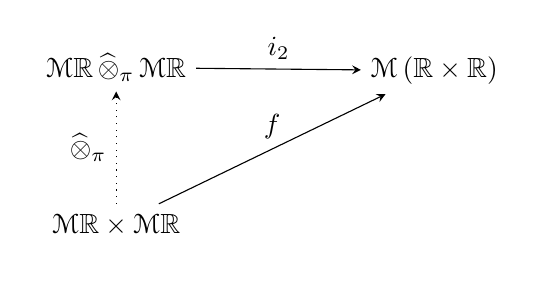
\begin{tikzpicture}
      \matrix (m) [matrix of math nodes, row sep=4em, column sep=6em, minimum width=2em]
      {
         \mathcal{M}\mathbb{R} \,   \widehat{\otimes}_{\pi} \,   \mathcal{M}\mathbb{R} &  \mathcal{M} \left( \mathbb{R} \times \mathbb{R} \right)  \\
        \mathcal{M}\mathbb{R} \times \mathcal{M}\mathbb{R}   \\
      };
      \path[dotted, -stealth]
      (m-2-1) edge node [left] {$\widehat{\otimes}_{\pi}$} (m-1-1);
      \path[-stealth]
        (m-1-1) edge node [above] {$i_2$} (m-1-2)
        (m-2-1) edge node [above] {$f$} (m-1-2)
        ;
    \end{tikzpicture}

    Where $i_2:  \mathcal{M}\mathbb{R} \,   \widehat{\otimes}_{\pi} \,   \mathcal{M}\mathbb{R} \to  \mathcal{M} \left( \mathbb{R} \times \mathbb{R} \right) $ is an isomorphism defined as $i_{2}( \mu  \widehat{\otimes}_{\pi} \nu ) = \mu \otimes \nu $ 
    and the function $f: \mathcal{M}\mathbb{R} \times \mathcal{M}\mathbb{R}  \to \mathcal{M} \left( \mathbb{R} \times \mathbb{R} \right) $ is defined as $f((\mu, \nu)) = \mu \otimes \nu $. 
    The product measure $\mu \otimes \nu$ is defined as $\mu \otimes \nu (A \times B)= \mu(A)\cdot\nu(B).$
      This is the measure produced by the Carath\'{e}odory's extension theorem \cite{aliprantisBanachLattices1999}.
       Given that $\norm{\mu \otimes \nu}= \norm{\mu} \cdot \norm{\nu}$,  and $\norm{(\mu, \nu)}= \max\{\norm{\mu}, \norm{\nu}\}$, for $\norm{\mu} \leq 1$ and $\norm{\nu} \leq 1$, it follows that $f$ is a short map.

    \end{comment}

    Since the diagram below commutes, and all the operations involved are short maps (considering $f$ as $\sem{\emph{delta}_r}$ or $\sem{\emph{u}_{r,s}}$), it follows that, if $d(\mu, \mu')=\epsilon$, then we may postulate \(\emph{JumpL}_\mu =_{\epsilon} \emph{JumpL}_{\mu'}\). A similar diagram can be constructed using \(jr_{*}\), allowing us to apply the same reasoning to the corresponding axioms.

    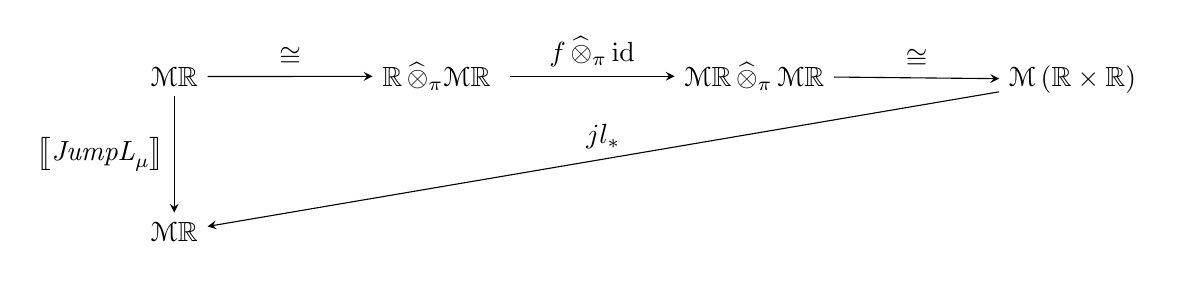
\begin{tikzpicture}
      \matrix (m) [matrix of math nodes, row sep=4em, column sep=6em, minimum width=2em]
      {
        \mathcal{M}\mathbb{R}  & \mathbb{R} \,   \widehat{\otimes}_{\pi} \mathcal{M}\mathbb{R} \,  \, & \mathcal{M}\mathbb{R} \, \widehat{\otimes}_{\pi} \,  \mathcal{M}\mathbb{R} &  \mathcal{M} \left( \mathbb{R} \times \mathbb{R} \right)  \\
        \mathcal{M}\mathbb{R}  \\
      };
      \path[-stealth]
        (m-1-1) edge node [left] {$\sem{\emph{JumpL}_\mu}$} (m-2-1)
        (m-1-1) edge node [above] {$\cong$} (m-1-2)
        (m-1-2) edge node [above] {$f\,  \widehat{\otimes}_{\pi} \,  \id $} (m-1-3)
        (m-1-3) edge node [above] {$\cong$} (m-1-4)
        (m-1-4) edge node [above] {$jl_{*}$} (m-2-1)
        ;
    \end{tikzpicture}

   We now present examples of \(\mu\) and \(\mu'\), and demonstrate how to compute the distance between them.
    First, consider $\mu=\delta_x$ and  $\mu'=\delta_y$. We calculate

    \begin{align*}
      \norm{\delta_x - \delta_y} = \sup \left\{ \sum_{i=1}^{n} |\delta_x - \delta_y (A_i)| \mid A_i \in \mathcal{B}(\mathbb{R}), A_i \cap A_j = \emptyset i,  \neq j, n \in \mathbb{N}  \right\} = 2
    \end{align*}
    Note that there are only two possibilities: either \(\delta_x\) and \(\delta_y\) belong to the same partition, or they belong to different ones. In the first case, we have
    \[
    \sum_{i=1}^{n} \left| \delta_x(A_i) - \delta_y(A_i) \right| = |1 - 1| = 0,
    \]
    while in the second case, we obtain
    \[
    \sum_{i=1}^{n} \left| \left( \delta_x(A_i) - \delta_y(A_i) \right) \right| = |1| + |-1| = 2.
    \]
    
    Next, take $\mu= \sum_{i=1}^{n} p_i \delta_{x_i}$ and  $\mu'= \sum_{i=1}^n q_i \delta_{x_i}$. We compute

    \begin{align*}
      \norm{\sum_i p_i \delta_{x_i} - \sum_i q_i \delta_{x_i}} &
      = \sup \left\{ \sum_{i=1}^{n} \left\lvert \left(\sum_i p_i \delta_{x_i} - \sum_i q_i \delta_{x_i} \right) (A_i) \right\rvert \,\Bigg| \, A_i \in \mathcal{B}(\mathbb{R}), A_i \cap A_j = \emptyset i,  \neq j, n \in \mathbb{N}  \right\} \\
      & = \sum_i |p_i-q_i|
    \end{align*}
    Here, we apply the same reasoning as in the previous example, while also using the inequality
\[
\left| \sum_{i=1}^{n} a_i \right| \leq \sum_{i=1}^{n} |a_i|, \quad \text{for all } n \in \mathbb{N}.
\]

Subsequently, let $\mu = U(a,b)$ and  $\mu'=U(c,d)$, such that the intervals $[a,b]$ and $[c,d]$ are disjoint ($[a, b] \cap [c, d] = \emptyset$). Then, the Radon-Nikodym derivatives (probability density functions) with respect to \( \nu = U(a, b) + U(c, d) \) are given by:

\[
\frac{dU(a, b)}{d\nu}(x) = u(a,b)(x) = 
\begin{cases} 
\frac{1}{b - a} & \text{if } x \in [a, b], \\ 
0 & \text{otherwise},
\end{cases}
\]
and similarly,
\[
\frac{dU(c, d)}{d\nu}(x) = u(c,d)(x) = 
\begin{cases} 
\frac{1}{d - c} & \text{if } x \in [c, d], \\ 
0 & \text{otherwise}.
\end{cases}
\]

Here, similarly to the first example, we calculate
\begin{align*}
  &\norm{U(a,b)-U(c,d)} = 2 \cdot \sup_{A \in \mathcal{B}(\mathbb{R})}  \left\{ \left\vert\int_A (u(a,b)(x)- u(c,d)(x)) \, d \nu(x) \right\vert \right\} \\
  & = 2 \cdot \sup_{A \in \mathcal{B}(\mathbb{R})}  \left\{ \left\vert\int_A (u(a,b)(x)) \, d \nu(x)  - \int_A (u(c,d)(x)) \,  d\nu(x) \right\vert \right\} = 2
\end{align*}

\begin{comment}
Here, we calculate
\begin{align*}
  \norm{U(a,b)-U(c,d)} = 2 \cdot \sup_{A \in \mathcal{B}(\mathbb{R})}  \left\{ \left\vert\int_A (u(a,b)(x)- u(c,d)(x)) \, dx \right\vert \right\} = 2 \cdot \sup_{A \in \mathcal{B}(\mathbb{R})}  \left\{ \left\vert\int_A (u(a,b)(x)- u(c,d)(x)) \, dx \right\vert \right\}
\end{align*}

In this case, we consider three scenarios: 
\begin{enumerate}
    \item The intervals are disjoint: \([a, b] \cap [c, d] = \emptyset\),
    \item One interval is fully contained in the other: for example, \([c, d] \subseteq [a, b]\) (or vice versa),
    \item The intervals intersect, but neither is fully contained in the other.
\end{enumerate}

In the first case, we have
\begin{align*}
  \int |u(a,b)(x)- u(c,d)(x)| \, dx  & = \int_a^b |u(a,b)(x)- u(c,d)(x)| \, dx + \int_c^d |u(a,b)(x)- u(c,d)(x)| \, dx \\
  & = \left\lvert \frac{b-a}{b-a}\right\rvert + \left\lvert- \frac{d-c}{d-c}\right\rvert = 2
\end{align*}

Regarding the second case, we compute
\begin{align*}
  \int |u(a,b)(x)- u(c,d)(x)| \, dx  & = \int_a^c |u(a,b)(x)- u(c,d)(x)| \, dx + \int_c^d |u(a,b)(x)- u(c,d)(x)| \, dx  \\
   & \hspace{10pt }+\int_d^b |u(a,b)(x)- u(c,d)(x)| \, dx \\
  & =  =  \frac{c-a}{b-a} + - (d-c) \left(\frac{1}{b-a} - \frac{1}{d-c}  \right)+  \frac{b-d}{b-a}
\end{align*}

At last, we calculate,
\begin{align*}
  \int |u(a,b)(x)- u(c,d)(x)| \, dx  & = \int_a^c |u(a,b)(x)- u(c,d)(x)| \, dx + \int_c^b |u(a,b)(x)- u(c,d)(x)| \, dx  \\
   & \hspace{10pt }+\int_b^d |u(a,b)(x)- u(c,d)(x)| \, dx \\
  & =  \frac{c-a}{b-a} +  (b-c) \left(\frac{1}{b-a} - \frac{1}{d-c}  \right)+  \frac{d-b}{b-a}
\end{align*}

\end{comment}

Finally, consider $\mu = \delta_{x_0} $  and $\mu' =  U(x_0 - \epsilon, x_0 + \epsilon) $. Let \(\nu = \delta_{x_0} + U(x_0 - \epsilon, x_0 + \epsilon) \). The Radon-Nikodym derivatives are:

\[
\frac{d\delta_{x_0}}{d\nu}(x) = f (x)
\begin{cases} 
1 & \text{if } x = x_0, \\
0 & \text{otherwise},
\end{cases}
\]

\[
\frac{dU(x_0 - \epsilon, x_0 + \epsilon)}{d\nu}(x) = u(x_0 - \epsilon, x_0 + \epsilon) = 
\begin{cases} 
\frac{1}{2\epsilon} & \text{if } x \in (x_0 - \epsilon, x_0 + \epsilon), \\
0 & \text{otherwise}.
\end{cases}
\]

We compute,
\begin{align*}
  \norm{\delta_{x_0}-U(x_0 - \epsilon, x_0 + \epsilon)} &= \sup_{A \in \mathcal{B}(\mathbb{R})} \left\{ \left\vert \int_A (f(x)- u(x_0 - \epsilon, x_0 + \epsilon) (x))\, d\nu(x) \right\vert \right\} \\
  &= \sup_{A \in \mathcal{B}(\mathbb{R})} \left\{ \left\vert \int_A f(x)\, d\nu(x) -  \int_A   u(x_0 - \epsilon, x_0 + \epsilon) (x) \, d\nu(x) \right\vert \right\} = 2
\end{align*}
    

\subsection{Finite-Dimensional Quantum Computation}

\todo[inline]{Adicionar os preliminares de computação quantica: notação, esfera de Bloch , ops pos, unitarios, op densidade (e conversão ops densidade bloch vector), ops kraus, quantum channels +  cenas de algebra linear: traço e norma euclidiana}

\vspace*{10pt}

The category $\catCPTP$ of completely positive trace-preserving maps is a symmetric monoidal category enriched over metric spaces \cite{dahlqvist2023syntactic}. The objects are natural numbers $n \geq 1$ and morphisms $n \rightarrow m$ are quantum channels $C^{n \times n} \rightarrow C^{m\times m}$.  An obvious candidate for the interpretation of quantum programs with coproducts is the category obtained by the coproduct cocompletion of $\catCPTP$,  $\catCPTP^{+}$ . In this setting, the $L^{\infty}$-norm arises as the natural metric. 


However, coproducts alone are insufficient to express the measurement operation which maps a density matrix $ \rho \in \mathbb{C}^{2 \times 2}$ to a classical bit $b \in \mathbb{C} \oplus \mathbb{C}$. To properly capture such operations, the category must also be equipped with products. However $\catCPTP$ does not have products. As a result, we consider category $\catCPS$, the category of completely positive trace-nonincreasing maps which is a symmetric monoidal category  \cite{selinger04}. The category $\catCPS^{+}$ is constructed analogously to $\catCPTP^{+}$. A version of $\catCPS$ with biproducts can be constructed via the dual of the coproduct cocompletion of $(\catCPS^{+})^{\cop}$.  The resulting category is denoted $\catCPS^{\oplus}$. Here, we may consider two natural candidates metrics for products: the $L^{\infty}$-norm and the $L^{1}$-norm. These correspond, respectively, to the following metrics: $d(\langle \phi, \psi \rangle, \langle \phi', \psi' \rangle ) = \sup \{ d(\phi, \phi' ), d(\psi, \psi') \}$ and $d(\langle \phi, \psi \rangle, \langle \phi', \psi' \rangle ) = d(\phi, \phi' ) +  d(\psi, \psi') $.

Let us start by verifying if the  $L^{\infty}$-norm is a suitable candidate for making $\catCPS^{\oplus}$ a $\catMet$-enriched category. For instance, for CPS maps $\phi_1, \phi_2,  \phi_1', \phi_2', \psi_1, \psi_2$ the following should hold:
\begin{align*}
  d([\psi_1, \psi_2] \cdot \langle \phi_1, \phi_2 \rangle, [\psi_1, \psi_2] \cdot \langle \phi_1', \phi_2' \rangle ) \leq d(\langle \phi_1, \phi_2 \rangle, \langle \phi_1', \phi_2' \rangle )
\end{align*}
Considering $\phi_1=\phi_2$, $\phi_1'=\phi_2'$, $\phi_1 \neq \phi_1'$ and $\psi_1= \psi_2 = \id$, we have
\begin{align*}
  & d([\psi_1, \psi_2] \cdot \langle \phi_1, \phi_2 \rangle, [\psi_1, \psi_2] \cdot \langle \phi_1', \phi_2' \rangle ) \\
  & = d(\psi_1 \cdot \phi_1 + \psi_2 \cdot \phi_2, \psi_1 \cdot \phi_1' + \psi_2 \cdot \phi_2') \\
  & = d(2 \phi_1, 2 \phi_1') 
\end{align*}

Futhermore, if the metric is induced by a norm, $\ie$ $d (\psi_1, \psi_2) = \lVert \psi_1 - \psi_2\lVert$ it follows that

\begin{align*}
  & d(2 \phi_1, 2 \phi_1') \\
  & = \lVert 2 \phi_1 - 2 \phi_1' \lVert \\
  & = 2 \cdot \lVert \phi_1 - \phi_1' \lVert \\
  & = 2 \cdot  d(\phi_1, \phi_1') > d(\phi_1, \phi_1') = \sup \{d(\phi_1, \phi_1'), d(\phi_2, \phi_2')\} = d(\langle \phi_1, \phi_2 \rangle, \langle \phi_1', \phi_2' \rangle )
\end{align*}

Thus, the $L^{\infty}$-norm is not a suitable candidate for making $\catCPS^{\oplus}$ a $\catMet$-enriched category. Now let us consider the $L^{1}$-norm. For CPS maps $ \phi, \phi', \phi_1, \phi_2$ the following should hold:
\begin{align*}
  d( \langle \phi_1, \phi_2 \rangle \cdot \phi, \langle \phi_1, \phi_2 \rangle \cdot \phi' ) \leq d(\phi, \phi')
\end{align*}

Considering $\phi_1=\phi_2 = \id$ and $\phi \neq \phi'$, we have
\begin{align*}
  & d( \langle \phi_1, \phi_2 \rangle \cdot \phi, \langle \phi_1, \phi_2 \rangle \cdot \phi' )  \\
  & = d(  \langle \phi_1 \cdot \phi, \phi_2 \cdot \phi \rangle \langle \phi_1 \cdot \phi', \phi_2 \cdot \phi' \rangle ) \\
  & = d(  \langle  \phi, \phi \rangle, \langle  \phi',  \phi' \rangle  )  \\
  & = d(  \phi,  \phi'  ) +  d(  \phi,  \phi'  ) \\
  & = 2 \cdot d(  \phi,  \phi'  ) > d(  \phi,  \phi'  )
\end{align*}

Given that none of the ``natural'' metrics are suitable for making $\catCPS^{\oplus}$ a $\catMet$-enriched category, we must now consider a metric between the $L^{\infty}$-norm and the $L^{1}$-norm, \ie, $$\sup \{ d(\phi, \phi' ), d(\psi, \psi') \} \leq d(\langle \phi, \psi \rangle, \langle \phi', \psi' \rangle ) \leq d(\phi, \phi' ) +  d(\psi, \psi').$$

In order to verify if this metric is valid,  we must ensure that for CPS maps $\phi_1, \phi_2,  \phi_1', \phi_2', \psi_1, \psi_2$ the following holds:
\begin{align*}
  d([\psi_1, \psi_2] \cdot \langle \phi_1, \phi_2 \rangle, [\psi_1, \psi_2] \cdot \langle \phi_1', \phi_2' \rangle ) \geq \sup \{ d(\phi_1, \phi_1' ), d(\phi_2, \phi_2') \}
\end{align*}

Assuming \(\phi_2 = \phi_2'\), that the metric is induced by a submultiplicative norm with respect to composition, and that \(\|\phi_1\| < 1\), we have
\begin{align*}
  & d([\psi_1, \psi_2] \cdot \langle \phi_1, \phi_2 \rangle, [\psi_1, \psi_2] \cdot \langle \phi_1', \phi_2' \rangle ) \\
  & = d(\psi_1 \cdot \phi_1 + \psi_2 \cdot \phi_2, \psi_1 \cdot \phi_1' + \psi_2 \cdot \phi_2') \\
  & = \lVert \psi_1 (\phi_1- \phi_1' ) \lVert \\
  & \leq    \lVert \psi_1  \lVert  \lVert \phi_1- \phi_1'  \lVert \\
  & = \lVert \phi_1- \phi_1'  \lVert  \\
    & =  d(\phi_1, \phi_1' )
\end{align*}

Consequently this norm is not fit either.


\begin{comment}


For instance, consider the trace norm, denoted $\tracenorm{-}$. Let $V$ and $W$ be finite-dimentional euclidean spaces and let $\mathcal{L}(V)$ denote the space of linear operators mapping a complex Euclidean space $V$ to itself.
This norm is defined on operators $ A:V \to V $ and superoperators  $\phi:\mathcal{L}(V) \to \mathcal{L}(W)$ as follows:
$$ \tracenorm{A} = \tr\left(\sqrt{A^\dagger A}\right) = \sum_i \tracenorm{A_i}  $$
$$ \sup \left\{ \tracenorm{\phi(A)} \, \vert \, \lVert A \lVert_{1} = 1 \right\}$$
Let $\psi_1$ be the trace operator and $\phi_1 = \id $ and $\phi_1' = D_p $, where $D_p: \mathbb{C}^2 \to \mathbb{C}^2$ is defined as 
\begin{align*} \label{eq:dephasing_result}
  &D_p(|\alpha|^{2} \ket{0} \bra{0} + \alpha \beta^{*} \ket{0} \bra{1}+ \alpha^{*} \beta \ket{1} \bra{0} + |\beta|^{2} \ket{1} \bra{1})  \\
  = &|\alpha|^{2} \ket{0} \bra{0} +  (1-p) \alpha \beta^{*} \ket{0} \bra{1}+  (1-p) \alpha^{*}  \beta \ket{1} \bra{0} + |\beta|^{2} \ket{1} \bra{1}. 
\end{align*}
 Then, $\phi_1 - \phi_1'$ maps a density operator 
$$\rho=|\alpha|^{2} \ket{0} \bra{0} + \alpha \beta^{*} \ket{0} \bra{1}+ \alpha^{*} \beta \ket{1} \bra{0} + |\beta|^{2} \ket{1} \bra{1}$$ 
to 
$$ p \cdot (\alpha \beta^{*} \ket{0} \bra{1}+ \alpha^{*} \beta \ket{1} \bra{0}).$$ 
The trace norm of $\phi_1 - \phi_1'$ is 
\begin{align*}
  & \left\lVert I - D_p\right\rVert_{1} \\
  & =  \max \limits_{\alpha, \beta} \left\lVert p \cdot  \left(\alpha \beta^{*}\ket{0}  \bra{1}+ \alpha^{*} \beta \ket{1} \bra{0}\right)\right\rVert_{1} \\
& = p \cdot \max \limits_{\alpha, \beta} \tr \left( \left(|\alpha|^2 |\beta|^2 \ket{0} \bra{0} + |\alpha|^2 |\beta|^2 \ket{1} \bra{1}\right)^{1/2} \right) \\
& =  p \cdot  \max \limits_{|\alpha|, |\beta| } 2 \cdot (|\alpha| |\beta|)  \\
& = p
\end{align*}
%Nota: Qualquer input poder ser escrito como a diferenca de estados puros com coeficientes, neste caso é muito claro que a norma é maximizada quando temos um estado puro.
On the other hand, it is evident that $\left\lVert \tr \left(  I - D_p \right) \right\rVert_{1}  =0$. Therefore, this metric is also not valid. As a result, we must consider a different approach.




\todo[inline]{Explicar melhor o op de Dephasing}

\end{comment}



%is the category $\catCPS$ of completely positive trace-preserving short maps 

%\todo{parte 2}
In \cite{selinger04}, Selinger presents the category $\catQ$ as the model of the language QPL.  

\begin{definition} \label{def:catQ}
  The category $\catQ$ is defined as the the finite biproduct completion of $\catCP$ (which extends $\catCPTP$ to include all completely positive maps),  further restricted to trace-nonincreasing morphisms. Let  $\mathcal{M}_n$ denote the set of complex $n\times n$ matrices.
  \begin{itemize}
    \item An object is a signature $\sigma= n_1, \ldots, n_s$. We denote these signatures by the Greek letters $\sigma, \tau$ and $\mu$.
    \item A morphism $\phi \in \sigma \to \tau $ is a matrix
    $$\begin{pmatrix}
      \phi_{11} & \ldots & \phi_{s1}, \\
      \vdots & \ddots  & \vdots \\
      \phi_{1t} & \ldots & \phi_{ts} \\
    \end{pmatrix}$$
    of arrows $\phi_{ij}: \mathcal{M}_{n_i} \rightarrow \mathcal{M}_{m_j}$ in $\catCPS$ which is trace-nonincreasing, \ie, the following condition holds:
    $$ \sum_j \sum_i \tr \left(\phi_{ij} (A_i)\right)   \leq  \sum_i \tr \left(A_i\right) $$
   for all positive $A_i \in \mathcal{M}_{n_i}$.

    More concretely, $ij$-component of $\phi$ is given by the function $\phi_{ij} = \pi_{j} \comp \phi \comp \mathrm{in}_{i} : \mathcal{M}_{n_i} \rightarrow \mathcal{M}_{n_j} $, where $\mathrm{in}_{i}$ is the injection of  $\mathcal{M}_{n_i}$ into the input space of $\phi$ and  $\pi_{j}$ is the projection onto the $j$-th component.
  \end{itemize}
\end{definition}


 Trace-non increasing (or short) maps are used here instead of strictly trace-preserving maps to account for possible non-termination in programs, particularly since the language  QPL includes while loops. Note that an operator $ \phi $ is called \emph{short} if $\norm{\phi} \leq 1$.


 Every signature $\sigma$, is associated to  a complex vector space:
\[
\mathcal{M}_\sigma = \mathbb{C}^{n_1 \times n_1} \oplus \cdots \oplus \mathbb{C}^{n_s \times n_s}.
\]
This space consists of matrix vectors 
$$A = \begin{pmatrix} A_1 \\ \vdots \\ A_n \end{pmatrix}$$
where the signature $\sigma$ specifies both the number of matrices, $s$,  and their respective dimensions, $n_i \times n_i$. The elements of $\mathcal{M}_\sigma$ are represented uppercase letters such as $A$, $B$, etc.
We also establish that
\[
\mathbb{C}^\sigma = \mathbb{C}^{n_1} \oplus \cdots \oplus \mathbb{C}^{n_s}.
\]

Note that attending to the definition of trace, for $A = \begin{pmatrix} A_1 & \ldots & A_n \end{pmatrix}^T$, $\tr(A) = \sum_i \tr(A_i).$
 



\begin{definition} \label{def:tensor} \emph{Tensor Product }
  For signatures $\sigma = n_1, \ldots, n_s $ and $\tau= m_1, \ldots, m_t $, the tensor product of $\sigma$ and $\tau$ is defined as $\sigma \otimes \tau = n_1 m_1, \ldots ,n_1 m_t, \ldots, n_s m_1,...,n_s m_t$. 
  The morphism part of the tensor product follows the definition in the category of vector spaces. If $\phi: \sigma \rightarrow \tau$ and $\psi: \sigma' \rightarrow  \tau'$, then their tensor product $\psi \otimes \phi: \sigma \otimes \sigma' \rightarrow  \tau \otimes \tau' $ is defined on a basis element $A \otimes B$ by  
$$
(\phi \otimes \psi)(A \otimes B) = F(A) \otimes G(B),
$$
and extends to arbitrary elements by linearity.
\end{definition}

\begin{definition} \label{def:biproduct} \emph{Product and Coproduct}
  The biproduct is given by the direct sum $\oplus$. Consequently, $\sigma \oplus \sigma'$ represents the concatenation of signatures. The co-pairing map $[\phi, \psi]: \sigma \oplus \sigma' \to \tau$ is defined as  $[\phi, \psi](A, B) = \phi(A) + \psi(B)$, and the pairing map $\langle \phi, \psi \rangle: \sigma \to \tau \oplus \tau'$ is given by  $\langle \phi, \psi \rangle(A) = (\phi(A), \psi(A))$.
\end{definition}

The category $\catQ$ is a distributive symmetric monoidal category with (finite) biproducts. Now, we must prove that $\catQ$ is a $\catMet$-enriched category. We consider the diamond norm on superoperators $\phi: \sigma \rightarrow \mu$ \cite{watrous2018theory}, given by:
 $$\diamondnorm{\phi} = \tracenorm{ \phi \otimes \id_{\mathcal{M}}}.$$

 Recall that the norm on a vector space induces a metric, in particular we obtain a metric $d$ on the hom-set \(\mathbf{Q}(\sigma, \tau)\),  which is defined by,
\[
d(\phi, \psi) = \diamondnorm{\phi, \psi},
\]
for \( \phi, \psi \in \mathbf{Q}(\sigma, \tau) \).



\begin{proposition} \label{prop:met_cond}
  For all $\phi, \phi' \in \catQ(\sigma,\mu)  $ and $\psi, \psi' \in \catQ(\tau,\mu) $, $[\phi-\phi',\psi-\psi']:\catQ(\sigma,\mu) \otimes \catQ(\tau,\mu) \rightarrow \catQ(\sigma \oplus \tau,\mu) $ is a functor in the category of metric spaces.
\end{proposition}



\begin{proof}
  We deduce by unfolding the respective definitions that we need to prove that for all short operators $\phi, \phi' \in \catQ(\sigma,\mu)  $ and $\psi, \psi' \in \catQ(\tau,\mu) $ the inequation $\diamondnorm{[\phi, \psi] - [\phi', \psi']} \leq  \sup \left\{ \diamondnorm{\phi-\phi'}, \diamondnorm{\psi-\psi'} \right\}$ holds.
 

    \begin{align*}
      & \gendiamondnorm{[\phi, \psi]} \\
      &= \tracenorm{[\phi, \psi] \otimes \id_{\sigma\oplus\tau}} \\
      &= \tracenorm{[\phi \otimes \id_\sigma, \psi \otimes \id_\tau]}& (\dist=\id) \\
      & =  \sup \{ \tracenorm{\phi \otimes \id_\sigma}, \tracenorm{\psi \otimes \id_\sigma} \} & (\text{Lemma \ref{lem_op_max_trace}})\\
      & = \sup \left\{ \diamondnorm{\phi}, \diamondnorm{\psi} \right\}
    \end{align*}

% The supremum of a set with two elements is always the maximum
  
The inequality in Proposition \ref{prop:met_cond} follows from the linearity of the co-pairing map.
\end{proof}


  \begin{corollary} \label{cor:gen_diamond_cptp_norm}
    Let $\sigma: n_1, \ldots, n_s$ and  $\tau: m_1, \ldots, m_t$  be signatures. Let  $\phi: \sigma  \rightarrow \tau$ be a  completely positive trace-nonincreasing super-operator. 
  \end{corollary}
  

  \begin{proof}
    Given that $\phi$ is a  completely positive trace-nonincreasing super-operator, if follows that $ \phi \otimes \id_{\sigma}$ is a positive trace-nonincreasing super-operator. Let $\psi = \phi \otimes \id$, it holds that,
    \begin{align*}
      \diamondnorm{\phi}& =\tracenorm{\psi}\\
       &= \max \left\{\tr \left( \psi (u u^\dag)\right) \, \vert \, \euclideannorm{u}=1 \right\}  & \left(\text{\cite[Theorem 3.39]{watrous2018theory}}\right)\\
      & = \max \left\{ \sum_i \sum_j \tr \left( \psi_{ij} (u_i u_i^\dag)\right) \Bigm|  \euclideannorm{\begin{pmatrix} u_1, \ldots, u_s^2 \end{pmatrix}^T}=1 \right\} \\
      & \leq \max \left\{ \sum_i \tr \left( u_i u_i^\dag \right) \Biggm| \sqrt{\sum_i \euclideannorm{u_i}^2}=1 \right\}   & (\psi \text{ is trace-nonincreasing}) \\
      & = 1
    \end{align*}
    
    % isto é verdade porque tr(u_iu_i^\dag ) =  \\ u_i\\^2 . consideremos u_i= (a_1,...,a_n), tr(ui)= |a_1|^2+...+ |a_n|^2 e \\ u_i\\ = \sqrt(|a_1|^2+...+ |a_n|^2)
    
    
  \end{proof}

  

\begin{proposition}
  The category $\catQ$ is $\catMet$-enriched and the bifunctor $\otimes : \catQ \otimes \catQ \to \catQ$ is $\mathsf{Met}$-enriched as well.
\end{proposition}



\begin{proof}
  First, we establish that $\catQ$ is $\catMet$-enriched. By unpacking the relevant definitions, this reduces to proving the following: for all short operators $\phi, \phi' : \sigma \to \tau$ and $\psi, \psi' : \tau \to \mu$ the inequation $\diamondnorm{\phi-\phi'} + \diamondnorm{\psi-\psi'} \geq \diamondnorm{\psi\phi-\psi'\phi'} $ holds. This follows directly from \cite[Proposition 3.38 (second statement)]{watrous2018theory}

  Next, regarding $\otimes$ we can also deduce by unfolding the respective definitions that we need to prove $ \diamondnorm{\phi - \phi'} + \diamondnorm{\psi - \psi'} \geq \diamondnorm{\psi \otimes \phi - \psi' \otimes \phi'}$. 
  For this case,  by \cite[Corollary 3.47]{watrous2018theory} and \cite[Proposition 3.44]{watrous2018theory} , we have the inequalities  
  \[
  \| \phi \|_\diamond \geq \| \phi \otimes \mathrm{id} \|_\diamond
  \quad \text{and} \quad  
  \| \phi \|_\diamond \geq \| \mathrm{id} \otimes \phi \|_\diamond
  \]  
  for any super-operator \( \phi \). Attending to \cite[ Proof of proposition 4.1]{dahlqvist2023syntactic} these conditions are sufficient to establish that the bifunctor $\otimes : \catQ \otimes \catQ \to \catQ$ is $\mathsf{Met}$-enriched.

  \todo[inline]{Versão longa para o tensor}

   Whith these conditions we calculate
  \begin{align*}
      \|\psi - \psi'\| + \|\phi - \phi'\| 
      &\geq \diamondnorm{\id \otimes \left(\psi-\psi'\right)} + \diamondnorm{\id \otimes \left(\phi-\phi'\right)}  \\
      &=  \diamondnorm{\id \otimes \psi- \id \otimes\psi'} + \diamondnorm{\id \otimes \phi- \id \otimes\phi'} \\
      &\geq \diamondnorm{\left( \id \otimes \psi \right) \cdot \left( \phi \otimes \id \right)} -  \diamondnorm{\left( \id \otimes \psi' \right) \cdot \left( \phi' \otimes \id \right)} & (\catQ \text{ is } \mathsf{Met}\text{-enriched}) \\
      &= \diamondnorm{\psi \otimes \phi - \psi' \otimes \phi'}
  \end{align*}

\end{proof}

$\catQ$ forms a model of the metric $\lambda$-theory for quantum computation introduced in  Subsection \ref{subsec:syntax_qc} via the following interpretation: $\sem{\typeI}= \mathbb{C} \ni  1$, 
$\sem{\emph{qbit} \hspace{1pt}}= \mathbb{C}^2$, 
$\sem{\emph{q} \hspace{1pt}}((a,b)) = \big(\begin{smallmatrix}
  a & 0\\
  0 & b
\end{smallmatrix}\big)$, 
for $\psi \in \{0, 1\}$ we define $\sem{\ket{\psi}} (1)= \ket{\psi} \bra{\psi}$,
$\sem{\emph{meas} \hspace{1pt}} (\rho)= (\text{Tr} (M_{0} \rho M_{0}^{\dag}), \text{Tr} (M_{1} \rho M_{1}^{\dag}))$, 
for unitary operations $U$ we define $\sem{U}= U \rho U^{\dag}$. 
For completely positive trace-preserving operators $CPTP$, defined as $CPTP (\rho) = K_0 \rho K_0^{\dag} +  K_1 \rho K_1^{\dag}$, we define  $\sem{CPTP}= CPTP (\rho)$ 

Since the diamond norm is generally difficult to compute, we will rely on the following properties, as given by the theorems below:

\begin{theorem} \cite[Theorem 3.55]{watrous2018theory} \label{theorem:diamond_iso}
  Let $\sigma: n_1, \ldots, n_s$ and  $\tau: m_1, \ldots, m_t$  be signatures for which is holds that $ \sum_i n_i \leq \sum_i m_i$, let $V_0,V_1: \mathbb{C}^{\sigma} \to \mathbb{C}^{\tau}$ be isometries, and define CPTP operators $\phi_0,\phi_1: \sigma \to \tau$ as
\[
\phi_0(X) = V_0XV_0^\dag \quad \text{and} \quad \phi_1(X) = V_1XV_1^\dag
\]
for all $X \in \mathcal{M}_\sigma$. There exists a unit vector $u \in \mathbb{C}^{\sigma} $ such that
\[
\tracenorm{\phi_0(uu^\dag) - \phi_1(uu^\dag)} = \diamondnorm{\phi_0 - \phi_1}.
\]
\end{theorem}

\begin{theorem} \cite[Theorem 3.56]{watrous2018theory} \label{theorem:diamond_cptp_id}
  Let $\sigma: n_1, \ldots, n_s$ be a signature. Let $\phi: \sigma \to \sigma $ be a quantum channel, let $\varepsilon \in [0,2]$, and suppose that
    \[
    \|\phi(\rho) - \rho\|_1 \leq \varepsilon
    \]
    for every density operator $\rho \in \mathcal{M}_\sigma$. It holds that
    \[
    \|\phi - \id_{\sigma}\|_1 \leq \sqrt{2\varepsilon}.
    \]
\end{theorem}

\begin{example}[Coin toss]
  When running a quantum program on a real quantum computer, the quantum circuits are mapped to the hardware's native quantum gates during compilation. For instance consider 2020 IBM's native quantum gate set $U_1,U_2,U_3,CX$ where

  \begin{align*}
    U_1(\lambda) &= 
    \begin{pmatrix}
        1 & 0 \\
        0 & e^{i\lambda}
    \end{pmatrix} \\
    U_2(\phi, \lambda) &= 
    \frac{1}{\sqrt{2}}
    \begin{pmatrix}
        1 & -e^{i\lambda} \\
        e^{i\phi} & e^{i(\phi+\lambda)}
    \end{pmatrix} \\
    U_3(\theta, \phi, \lambda) &= 
    \begin{pmatrix}
        \cos(\theta/2) & -e^{i\lambda}\sin(\theta/2) \\
        e^{i\phi}\sin(\theta/2) & e^{i(\phi+\lambda)}\cos(\theta/2)
    \end{pmatrix} \\
\end{align*}

Here, \( R_{y,\theta} \), representing a single-qubit rotation by an angle \( \theta \) around the y-axis, can be expressed as \( U_3(\theta, 0, 0) \). We now examine how the coin toss outcome is affected when the \( U_3 \) gate is faulty, particularly when its parameter \( \theta \) is perturbed by an error \( \epsilon \). In this case, the implemented gate becomes \( U_3(\theta + \epsilon, \phi, \lambda) \), \ie, $R_{y,\theta+\epsilon}$.
First, we compute the action of the unitary operator \( U_3(\theta, \phi, \lambda) \) on an arbitrary quantum state \( \ket{\psi} \).
\begin{align*}
  U_3(\theta, \phi, \lambda) \ket{\psi} 
  & = U_3(\theta, \phi, \lambda) \left(\cos(\alpha/2) \ket{0} + e^{i\beta}\sin(\alpha/2) \ket{1} \right)\\
  & = \left(\cos(\alpha/2) \cos(\theta/2) - e^{i (\lambda + \beta)}  \sin(\alpha/2)\sin(\theta/2) \right) \ket{0} \\
  & + \left(e^{i \phi}\cos(\alpha/2)\sin(\theta/2) + e^{i (\beta + \lambda + \phi)} \sin(\alpha/2) \cos(\theta/2 ) \right) \ket{1}
\end{align*}
Designating $U_3(\theta, \phi, \lambda) \ket{\psi} = a \ket{0} + b \ket{1}$, one has
\begin{align*}
  a a^* &= \vert \cos(\alpha/2) \cos(\theta/2) - e^{i (\lambda + \beta) }  \sin(\alpha/2)\sin(\theta/2) \vert ^2 \\
  &= \cos^2(\alpha/2) \cos^2(\theta/2) - 2 \cos(\beta + \lambda) \cos(\alpha/2) \cos(\theta/2)  \sin(\alpha/2)\sin(\theta/2) + \sin(\alpha/2)^2 \sin^2(\theta/2) \\
  & = \cos^2(\alpha/2) \cos^2(\theta/2) + \sin^2(\alpha/2) \sin^2(\theta/2)  - 1/2 \cos(\beta + \lambda) \sin(\alpha)\sin(\theta) \\
  & = \cos^2((\theta+\alpha)/2)+(1-\cos(\beta + \lambda))\sin(\alpha)\sin(\theta) -1 \\
  a^*b & = \left(\cos(\alpha/2) \cos(\theta/2) - e^{-i (\lambda + \beta)}  \sin(\alpha/2)\sin(\theta/2) \right) \left(e^{i \phi}\cos(\alpha/2)\sin(\theta/2) + e^{i (\beta + \lambda + \phi)} \sin(\alpha/2) \cos(\theta/2 ) \right) \\
  & = (1/2) \left( e^{i \phi} \cos^2(\alpha/2) \sin(\theta) + e^{i (\beta + \lambda + \phi)} \sin(\alpha) \cos^2(\theta/2) - e^{-i (\beta + \lambda -\phi)} \sin(\alpha) \sin^2(\theta/2) - e^{i \phi} \sin^2(\alpha/2) \cos(\theta/2)  \right) \\
  & = (1/2) \left( e^{i \phi}\cos(\alpha) \sin(\theta) +  \sin(\alpha) \left(e^{i (\beta + \lambda + \phi)} \cos^2(\theta/2) - e^{-i (\beta + \lambda - \phi)} \sin^2(\theta/2)\right)  \right)
\end{align*}
Then, we calculate the vector Bloch of $U_3(\theta, \phi, \lambda) \ket{\psi}$,
\begin{align*}
  &x = 2 \text{Im} \left( a^{*}b \right) =   \cos(\phi) \cos(\alpha) \sin(\theta) +  \sin(\alpha) \left(\cos{(\beta + \lambda + \phi)} \cos^2(\theta/2) - \cos{(\beta + \lambda - \phi)} \sin^2(\theta/2)\right)  \\
  &y = 2 \text{Re} \left( a^{*}b \right) = \sin(\phi) \cos(\alpha) \sin(\theta) +  \sin(\alpha) \left(\sin{(\beta + \lambda + \phi)} \cos^2(\theta/2) + \sin{(\beta + \lambda - \phi)} \sin^2(\theta/2)\right) \\
  & z = 2 aa^* -1 = 2 \cos^2((\theta+\alpha)/2)+(1-\cos(\beta + \lambda))\sin(\alpha)\sin(\theta) -1
\end{align*}
As a result, we have,
\begin{align*}
  & \tracenorm{U_3(\theta, 0, 0) \ket{\psi}\bra{\psi} U_3(\theta, 0, 0)^\dag - U_3(\theta + \epsilon, 0, 0) \ket{\psi}\bra{\psi}U_3(\theta+\epsilon, 0, 0)^\dag } \\
  & = \lVert ( \cos(\alpha) (\sin(\theta) - \sin(\theta + \epsilon)) +  \sin(\alpha) \cos{\beta} \left(\cos(\theta) - \cos(\theta + \epsilon) \right) , 0,\\
  & \hspace{20pt} 2 (\cos^2((\theta+\alpha)/2) - \cos^2((\theta+ \epsilon+\alpha)/2))+\cos(\beta) \sin(\alpha)(\sin(\theta) - \sin(\theta+\epsilon)) )\rVert_2 \\
  %& \leq \lVert  (\sin(\theta) - \sin(\theta + \epsilon) + \cos(\theta) - \cos(\theta + \epsilon),0, \\
  %&  \hspace{20pt}  2 (\cos^2((\theta+\alpha)/2) - \cos^2((\theta+ \epsilon+\alpha)/2))+(\sin(\theta) - \sin(\theta+\epsilon))) \rVert_2   \\
  &  \leq \euclideannorm{( \cos(\alpha)\epsilon + \sin(\alpha)\cos(\beta) \epsilon, 0, 2\epsilon + \sin(\alpha)\cos(\beta) \epsilon)} \\
  & = \sqrt{\epsilon^2(\cos^2(\alpha) + 2\sin^2(\alpha)\cos^2(\beta)+\sin(2\alpha)\cos(\beta) + 2\sin(\alpha)\cos(\beta) + 4 )} \\
  &\leq \epsilon \sqrt{(1 + \sin^2(\alpha) +\sin(2\alpha) + 2\sin(\alpha) + 4 )} \\
  & \leq \epsilon \sqrt{(1 + 4 + 4 )} = 3 \epsilon
\end{align*}

The first inequality arises from both functions $\cos$ and $\sin$ being Lipschitz continuous. Attending to Theorem \ref{theorem:diamond_iso}, it follows that
  \begin{align*}
    \diamondnorm{R_{y, \theta}- R_{y, \theta + \epsilon} } \leq 3 \epsilon
  \end{align*}

Using our metric deductive system, considering Example \ref{ex:coin_toss_syntax} we can easily conclude that $\textbf{CoinToss} =_{3 \epsilon} \textbf{CoinToss}^{\epsilon}$, where $\textbf{CoinToss}^{\epsilon}$ is the the judgement that results from replacing $R_{y, \theta}$ by $U^{R_{y, \theta + \epsilon}}$.

\end {example}

\begin{example}[Quantum state discrimination]
  An arbitrary single qubit unitary $U \in \mathbb{C}^{2 \times 2}$ may be written
\[
U = e^{i\alpha} R_{z,\beta} R_{y,\gamma} R_{z,\delta},
\]
for appropriate choices of angles $\alpha$, $\beta$, $\gamma$ and $\delta$.


As in the previous example, we assume the hardware's native gate set consists of $\{U_1, U_2, U_3, \text{CNOT}\}$, and the quantum circuit is compiled into these gates.  
As previously noted, the $R_y(\theta)$ gate can be implemented as $U_3(\theta, 0, 0)$.  
Similarly, the $R_z(\lambda)$ gate is equivalent to $U_1(\lambda)$ up to a global phase factor $e^{-i\lambda/2}$ which does not affect measurement outcomes. 
Therefore, it can be directly implemented using the $U_1$ gate.  
We will also consider that the gates $U_1$ and $U_3$ are affected by errors $\epsilon_1$ and $\epsilon_2$, respectively. 
More precisely, we will consider erroneous implementations of this gates $U_1(\lambda + \epsilon_1)$ and $U_3(\theta + \epsilon_2, \phi, \lambda)$. 
From the previous example, we know that the error in the $R_y$ gate is bounded by $3 \epsilon_2$. 
Consider the single-qubit state
\[
\ket{\psi} = \cos\left(\frac{\alpha}{2}\right)\ket{0} + e^{i\beta}\sin\left(\frac{\alpha}{2}\right)\ket{1}.
\]
Applying the \( U_1(\lambda) \) gate yields
\[
U_1(\lambda)\ket{\psi} = \cos\left(\frac{\alpha}{2}\right)\ket{0} + e^{i(\beta + \lambda)}\sin\left(\frac{\alpha}{2}\right)\ket{1}.
\]
The corresponding Bloch vector is then
\[
\left(\!\cos(\beta + \lambda)\sin\alpha,\; \sin(\beta + \lambda)\sin\alpha,\; \cos\alpha\right).
\]
Consequently, applying the same reasoning as in the previous example, it follows that
\begin{align*}
  & \tracenorm{U_1(\lambda) \ket{\psi}\bra{\psi} U_1(\lambda)^\dag - U_1(\lambda + \epsilon) \ket{\psi}\bra{\psi}U_1(\lambda + \epsilon)^\dag } \\
  & = \euclideannorm{\left(\sin(\alpha) \left( \cos(\beta + \lambda) -  \cos(\beta + \lambda + \epsilon) \right),\sin(\alpha) \left( \sin(\beta + \lambda) -  \sin(\beta + \lambda + \epsilon) \right),0 \right)} \\
  & \leq \euclideannorm{\left( \cos(\beta + \lambda) -  \cos(\beta + \lambda + \epsilon) , \sin(\beta + \lambda) -  \sin(\beta + \lambda + \epsilon) ,0 \right)} \\
  & \leq \euclideannorm{\left( \epsilon, \epsilon ,0 \right)} \\
  & = \sqrt{2}\epsilon \\
\end{align*} 

Attending to Theorem \ref{theorem:diamond_iso}, it follows that
  \begin{align*}
    \diamondnorm{U_1(\lambda)- U_1(\lambda + \epsilon) } \leq \sqrt{2} \epsilon
  \end{align*}


As a result, in  Example \ref{ex:quantum_state_discrimination_syntax}, considering the $\lambda$-term \textbf{HMeasure} and the erroneous implementation of $U$ described above, denoted $U^{\epsilon_1, \epsilon_2}$, using our deductive metric system, we have $U =_{\sqrt{2}\epsilon_1+ 3\epsilon_2} U^{\epsilon_1, \epsilon_2}$. Therefore, we deduce $\textbf{HMeasure} =_{\sqrt{2}\epsilon_1+ 3\epsilon_2} \textbf{HMeasure}^{\epsilon_1, \epsilon_2}$, where $\textbf{HMeasure}^{\epsilon_1, \epsilon_2}$ is the the judgement that results from replacing $U$ by $U^{\epsilon_1, \epsilon_2}$. Moreover, considering the erroneous implementation of the $R_y$ gate also afecting the \textbf{CoinToss} term, as discussed in the previous example, we deduce that 
$$\textbf{Discrimination} =_{\sqrt{2}\epsilon_1+6\epsilon_2} \textbf{Discrimination}^{\epsilon_1,\epsilon_2}, $$
where $\textbf{Discrimination}^{\epsilon_1,\epsilon_2}$ denotes the judgement that results from replacing $\textbf{HMeasure}$ by $\textbf{HMeasure}^{\epsilon_1, \epsilon_2}$ and $\textbf{CoinToss}$ by  $\textbf{CoinToss}^{\epsilon_2}$.

%\textbf{Discrimination}
\end{example}

  \begin{example}[Quantum teleportation]
    
  \todo[inline]{DUVIDA: Se tivermos dois programas g(f(x) e g'(f'(x))) (com f,g,f', g' a ser funções predeterminadas como unitários) temos que explicitamente reescrever so programas como g(f(x)/y) e  g'(f'(x)/y) para podermos usar a regra da substituição no sistema métrico?}


    Following the approach of previous examples, we analyze erroneous implementations of the gates $U_1$ and $U_3$ within the hardware’s native gate set. Additionally, consider the action of both dephasing and amplitude damping channels. Furthermore, we account for an adversarial agent that applies a bit-flip operation immediately prior to measurement with probability $ p = 0.5 $.  

    Here, we consider imperfect implementations of the gates $U_1$ and $U_3$, given by $ U_1(\lambda) $ and $ U_3(\theta, \phi + \epsilon_2, \lambda + \epsilon_3)$, respectively. 
    Recall from the previous example that we established the bound $\diamondnorm{U_1(\lambda)- U_1(\lambda + \epsilon) } \leq \sqrt{2} \epsilon$.
     The Hadamard gate, $H$, is the composition $U_3(\pi/2, 0, 0)\cdot U_1(\pi)$. We calculate,
    \begin{align*}
      &\tracenorm{U_3(\pi/2, 0, 0) \ket{\psi}\bra{\psi}U_3(\pi/2, 0, 0)^\dag - U_3(\pi/2, \epsilon_2, \epsilon_3)  \ket{\psi}\bra{\psi}U_3(\pi/2, \epsilon_2, \epsilon_3)^\dag} \\
      & = \lVert (\cos(\alpha)( 1-\cos{\epsilon_2}) + \sin(\alpha)( 1/2(\cos(\beta + \epsilon_2 + \epsilon_3)-\cos(\beta - \epsilon_2 + \epsilon_3))), \\
      & \hspace{20pt} \cos(\alpha)( 1-\sin{\epsilon_2}) + (1/2)\sin(\alpha) (\sin(\beta)-\sin(\beta+\epsilon_2 + \epsilon_3) + \sin(\beta)-\sin(\beta-\epsilon_2 + \epsilon_3)),   \\
      & \hspace{20pt} (\cos(\beta + \epsilon_3)-\cos(\beta))\sin(\alpha) ) \lVert_2 \\
      & \leq \euclideannorm{(\cos(\alpha) \epsilon_2 + (1/2)\sin(\alpha) (\epsilon_2 + \epsilon_3) ,\cos(\alpha) \epsilon_2 + (1/2)  \sin(\alpha) (\epsilon_2 + \epsilon_3 + |\epsilon_3-\epsilon_2|), \sin(\alpha) \epsilon_3)} \\
      &  < \euclideannorm{(\epsilon_2 + (1/2)(\epsilon_2 + \epsilon_3), \epsilon_2 + (1/2)   (\epsilon_2 + \epsilon_3 + |\epsilon_3-\epsilon_2|), \epsilon_3)}  \\
      & \leq 3 \epsilon_2 +  2\epsilon_3 + |\epsilon_2-\epsilon_3| \\
    \end{align*}

    Attending to Theorem \ref{theorem:diamond_iso}, it follows that
    \begin{align*}
      \diamondnorm{U_3(\pi/2, 0, 0)- U_3(\pi/2, \epsilon_2, \epsilon_3) } \leq 3 \epsilon_2 +  2\epsilon_3 + |\epsilon_2-\epsilon_3|
    \end{align*}
    
    As a result, denoting the imperfect implementation of the Hadamard gate as $H^{\epsilon_1 ,\epsilon_2, \epsilon_3}$, we have 
    \begin{align} \label{eq:h_error_telepor}
      H =_{ \sqrt{2}\epsilon_1 + 3 \epsilon_2 + 2\epsilon_3 + |\epsilon_2-\epsilon_3|} H^{\epsilon_1 ,\epsilon_2, \epsilon_3}.
    \end{align}
 

    The gate $X$ can be implemented as $U_3(\pi, \psi, 0)$. We compute,
    \begin{align*}
      &\tracenorm{U_3(\pi, 0 , \pi) \ket{\psi}\bra{\psi}U_3(\pi,0,\pi)^\dag - U_3(\pi,\epsilon_2,\pi+\epsilon_3)  \ket{\psi}\bra{\psi}U_3(\pi,\epsilon_2,\pi+\epsilon_3)^\dag}  \\
      & =\euclideannorm{( \sin(\alpha) (\cos(\beta)+\cos(\beta + \epsilon_3-\epsilon_2)), \sin(\alpha) (\sin(\beta + \epsilon_3-\epsilon_2)-\sin(\beta)),0 )} \\
      &  \leq \euclideannorm{(|\epsilon_3-\epsilon_2|, |\epsilon_3-\epsilon_2|,0 )} \\
      & = \sqrt{2} |\epsilon_3-\epsilon_2|
    \end{align*}

    Considering Theorem \ref{theorem:diamond_iso}, it holds that
    \begin{align*}
      \diamondnorm{U_3(\pi, 0 , \pi)- U_3(\pi,\epsilon_2,\pi+\epsilon_3) } \leq \sqrt{2} |\epsilon_3-\epsilon_2|
    \end{align*}

    As a result, denoting the erroneous implementation of the $X$ gate as $X^{\epsilon_2, \epsilon_3}$, we have
    \begin{align} \label{eq:x_error_telepor}
      X =_{\sqrt{2} |\epsilon_3-\epsilon_2|} X^{\epsilon_2, \epsilon_3}.
    \end{align}
  

    Finally, the gate $Z$ corresponds to $U_1(\pi)$, therefore, denoting the erroneous implementation of the $X$ gate as $X^{\epsilon_1}$, we postulate the following axiom
    \begin{align} \label{eq:Correction_error_telepor}
      Z =_{\sqrt{2} \epsilon_1} Z^{\epsilon_1}.
    \end{align}

    Designating the \textbf{Correction} block with the imperfect implementations of $X$ and $Z$ by $\textbf{Correction}^{\epsilon_1, \epsilon_2, \epsilon_3}$, in light of the axioms in equations \eqref{eq:x_error_telepor} and \eqref{eq:x_error_telepor} and our metric deductive system we have that
    \begin{align} \label{eq:z_error_telepor}
      \textbf{Correction} =_{\sqrt{2} \left(\epsilon_1 +|\epsilon_3-\epsilon_2| \right)} \textbf{Correction}^{\epsilon_1, \epsilon_2, \epsilon_3}.
    \end{align}


     \textbf{Dephasing channel}
     Realistic quantum systems are never isolated, but are immersed in the surrounding environment and interact continuously with it. Decoherence can be seen as the consequence of that  `openness' of quantum systems to their  environments .  To study decoherence in a quantum channel within the presented metric deductive system, one can consider the application of a dephasing channel in the quantum teleportation protocol with a certain probability $p$.
     
     The Kraus operators of the dephasing channel with probability $p$ are expressed as:
     \begin{equation*}
          D_{0}= \frac{\sqrt{2-p}}{\sqrt{2}} I,  D_{1}= \frac{\sqrt{p}}{\sqrt{2}} Z
     \end{equation*}
     
     Considering a density operator $\rho=|\alpha|^{2} \ket{0} \bra{0} + \alpha \beta^{*} \ket{0} \bra{1}+ \alpha^{*} \beta \ket{1} \bra{0} + |\beta|^{2} \ket{1} \bra{1}$, using these Kraus operators, it is possible to easily verify  that after applying the dephasing channel with probability $p$, the resulting operator $\rho'$ is given by: 
     \begin{equation*} 
          \rho' = D_p(\rho)= D_{0} \rho D_{0}^{\dag} + D_{1} \rho D_{1}^{\dag} = |\alpha|^{2} \ket{0} \bra{0} +  (1-p) \alpha \beta^{*} \ket{0} \bra{1}+  (1-p) \alpha^{*}  \beta \ket{1} \bra{0} + |\beta|^{2} \ket{1} \bra{1}
     \end{equation*}
     This shows that the dephasing channel with probability $p$ preserves the diagonal elements of the density matrix while attenuating the off-diagonal elements by a factor of $(1-p)$.

     In this scenario (and in subsequent ones), we will add identity gates to the ideal program to simplify the calculations. Thus, attending do the definition of trace norm for matrices, we have:
     \begin{align*}
      & \tracenorm{ \id(\rho) - D_{p}(\rho)} \\
      & \tracenorm{ \alpha \beta^{*} \ket{0} \bra{1}+ \alpha^{*} \beta \ket{1} \bra{0}  -   (1-p) \alpha \beta^{*} \ket{0} \bra{1}-  (1-p) \alpha^{*}  \beta \ket{1} \bra{0} } \\
      & = p \cdot  \tracenorm{ \alpha \beta^{*} \ket{0} \bra{1} + \alpha^{*}  \beta \ket{1} \bra{0} } \\
      & = p \cdot \tr \left(\sqrt{\left( \alpha \beta^{*} \ket{0} \bra{1} + \alpha^{*}  \beta \ket{1} \bra{0} \right)^2} \right) \\
      & = p \cdot  \tr \left(\sqrt{|\alpha|^{2}|\beta|^{2} (\ket{0} \bra{0}+ \ket{1} \bra{1})  } \right) \\
      & = 2 \cdot p \cdot |\alpha||\beta| \\
      & \leq p \\
     \end{align*}
     The last step arises from the fact that the expression is maximized when $|\alpha|=|\beta|=1/\sqrt{2}$.

     Considering Theorem \ref{theorem:diamond_cptp_id}, it holds that
     \begin{align*}
        \diamondnorm{ \id - D_p} \leq \sqrt{2p}
     \end{align*}

     Consequently, we can postulate the following axiom:
      \begin{align} \label{eq:dephasing_telepor}
         \id =_{\sqrt{2p}}  D_p  .
      \end{align}

     If a dephasing channel acts on the first qubit of the EPR state, we are interested in reasoning about the following judgements:
     \begin{align*}
      &\textbf{EPR} = (\id \otimes \id)(\emph{CNOT} (\emph{H}\ket{0},\ket{0})) : \emph{qbit} \otimes
      \emph{qbit}  \\ 
      %
      &\textbf{EPR}^{\epsilon_1,\epsilon_2, \epsilon_3,p} =  (D_p \otimes \id) (\emph{CNOT} ( \emph{H}^{\epsilon_1,\epsilon_2, \epsilon_3}\ket{0},\ket{0})) : \emph{qbit} \otimes
      \emph{qbit} 
   \end{align*}

   Given axioms in equations \eqref{eq:h_error_telepor} and \eqref{eq:dephasing_telepor}, using our metric deductive system, we infer that
   \begin{align} \label{eq:epr_error_teleport}
    \textbf{EPR} =_{\sqrt{2}\epsilon_1 + 3 \epsilon_2 + 2\epsilon_3 + |\epsilon_2-\epsilon_3| + \sqrt{2p}} \textbf{EPR}^{\epsilon_1,\epsilon_2, \epsilon_3,p}
   \end{align}


     \textbf{Amplitude Dephasing channel}
     Next, the amplitude-damping channel is considered as a source of noise in the quantum teleportation protocol. Similarly to the dephasing channel, the amplitude damping channel serves as a model illustrating the dissipation of energy between a qubit and its environment. An example of this type of noise is found in the spontaneous emission of a photon by a two-level atom into an electromagnetic field environment with either a finite or infinite number of modes at zero temperature \cite{salles2008experimental, Wang_2011}.

     The amplitude damping channel with probability $\gamma$ is described by the Kraus operators:
\begin{equation*}
     A_{0}= \ket{0} \bra{0} + \sqrt{1-\gamma} \ket{1} \bra{1} ,  A_{1}= \sqrt{\gamma} \ket{0} \bra{1}
\end{equation*}

Applying these Kraus operators an arbitray density operator $\rho=|\alpha|^{2} \ket{0} \ket{0} + \alpha \beta^{*} \ket{0} \ket{1} + \alpha^{*} \beta \ket{1} \ket{0} + |\beta|^{2} \ket{1} \ket{1}$, we obtain the state $\rho'$ as follows:
\begin{align*}
     \rho' & = A_\gamma(\rho) =  A_{0} \rho A_{0}^{\dag} + A_{1} \rho A_{1}^{\dag} \\
     & = (|\alpha|^{2} + \gamma |\beta|^{2}) \ket{0}\bra{0} + \sqrt{1-\gamma} \hspace{1pt} \alpha \beta^{*} \ket{0}\bra{1} + \sqrt{1-\gamma} \hspace{1pt} \alpha^{*} \beta \ket{1}\bra{0} + (1-\gamma) |\beta|^{2} \ket{1}\bra{1}
\end{align*}

Once again, we will add identity gates to the ideal program to simplify the calculations, as a result it is necessary to compute the trace norm of the diference between the identity applied to the density operator $\rho = \ket{\psi} \bra{\psi}$ and the amplitude damping channel applied to $\rho$.
First, we calculate, 
\begin{align*}
  & \tracenorm{ \id(\rho) - A_{\gamma}(\rho)} \\
  & =    \Big\lVert  |\alpha|^{2} \ket{0} \ket{0} + \alpha \beta^{*} \ket{0} \ket{1} + \alpha^{*} \beta \ket{1} \ket{0} + |\beta|^{2} \ket{1} \ket{1}  - \big((|\alpha|^{2} + \gamma |\beta|^{2}) \ket{0}\bra{0} \\ 
  & \hspace{10pt}  +  \sqrt{1-\gamma} \hspace{1pt} \alpha \beta^{*} \ket{0}\bra{1} + \sqrt{1-\gamma} \hspace{1pt} \alpha^{*} \beta \ket{1}\bra{0} + (1-\gamma) |\beta|^{2} \ket{1}\bra{1}\big) \Big\rVert_1 \\
   & = \tracenorm{\gamma |\beta|^{2} \ket{0} \bra{0} + (1-\sqrt{1-\gamma}) (\alpha \beta^{*} \ket{0} \bra{1} + \alpha^{*} \beta \ket{1} \bra{0}) - \gamma |\beta|^{2} \ket{1} \bra{1}} \\
   & = \tr \left( \sqrt{\left( \gamma |\beta|^{2} \ket{0} \bra{0} + (1-\sqrt{1-\gamma}) (\alpha \beta^{*} \ket{0} \bra{1} + \alpha^{*} \beta \ket{1} \bra{0}) - \gamma |\beta|^{2} \ket{1} \bra{1}  \right)^2}\right) \\
   & = \tr \left( \sqrt{\left( (1-\sqrt{1-\gamma})^{2} |\alpha|^{2}|\beta|^{2} + \gamma^{2} |\beta|^{4} \right) (\ket{0} \bra{0} + \ket{1} \bra{1} ) } \right) \\
   & = 2 \cdot \sqrt{  (1-\sqrt{1-\gamma})^{2} |\alpha|^{2}|\beta|^{2} + \gamma^{2} |\beta|^{4}} \\
   & \leq 2 \gamma
\end{align*}
This final step follows because the expression attains its maximum when 
∣$|\alpha|=0 $ and $|\beta|=0.$

Attending to Theorem \ref{theorem:diamond_cptp_id}, it holds that
\begin{align*}
  \diamondnorm{ \id - A_\gamma} \leq 2 \sqrt{\gamma}
\end{align*}

As a result, we can postulate the following axiom:

    \begin{align} \label{eq:amp_damp_teleport}
        \id =_{2 \sqrt{\gamma}} A_\gamma.
    \end{align}


When an amplitude damping channel acts on the final qubit following the Correction block, we define two new lambda terms consisting of the ideal operation \textbf{Id} and its erroneous counterpart  $\textbf{Id}^{\gamma}$.

\begin{align}\label{eq:id_error_teleport}
  &\textbf{Id} = qb:\textit{qbit} \, \vljud \id (qb) \\
  & \textbf{Id}^{\gamma} = A_{\gamma} (q):\textit{qbit} \, \vljud  A_{\gamma} (qb)
\end{align}


Consequently the ideal version of teleportation protocol is now defined as follows

\begin{align*} 
  \textbf{QTP} = qb_{0}: \textit{qbit}\hspace{3 pt} \vljud \hspace{3 pt} & \text{pm} \hspace{5pt} \textbf{EPR} \hspace{5pt} \text{to} \hspace{5pt}  qb_{1} \otimes qb_{2}.  \notag \\
     & \text{pm}\hspace{5pt} \textbf{BellMeasure}\, [qb_0/q_1,qb_{1}/q_2] \hspace{5pt}  \text{to} \hspace{5pt} c_{0}\otimes c_{1} . \notag \\
     & \textbf{Id} \, [ \textbf{Correction}/qb] \, [qb_{2}/q,c_{0}/x, c_{1}/y] 
     : \emph{qbit}  
 \end{align*}

 Considering the axiom in equation \eqref{eq:amp_damp_teleport} and our metric deductive system, it holds that 
\begin{align*}
  &\textbf{Id}=_{2 \sqrt{\gamma}} \textbf{Id}^{\gamma}
\end{align*}

\textbf{Malicious attack}
Finally consider a malicious attack on the quantum teleportation protocol in the form of a bit-flip occurring with a 50\% probability before measurement.
More generally,  one can define an operation $T$ that applies a unitary operation $U$ to the state given as input with 50\% probability. Operation $T$ can be defined as follows:
\begin{equation*}
\begin{split}
  &T: \hspace{5pt} \textit{qbit}  \to \textit{qbit} \\
  &T= q:\textit{qbit} \hspace{2pt} \vljud \text{pm} \hspace{2pt} CU ( R_{x,\frac{\pi}{2}}(\ket{0}) ,q) \hspace{2pt} \text{to} \hspace{2pt} newq \otimes qb. \hspace{2pt} \textit{disc} (newq) 
\end {split}
\end{equation*}
Here, $CU$ denotes the controlled operation that applies $U$ to the second qubit when the first qubit is in the state $\ket{1}\bra{1}$, and leaves it unchanged when the first qubit is in the state $\ket{0}\bra{0}$. The operator $R_{x,\frac{\pi}{2}}$ represents a rotation by $\frac{\pi}{2}$ around the x-axis of the Bloch sphere.


This operation is depicted in \autoref{fig:Operation_T}.

\begin{figure} [H]
  \centering
  \begin{quantikz} [column sep=0.2cm, row sep=0.5cm,wire
    types={n,n}]%
      \lstick{$\ket{\phi}$}  &\qw \gategroup[2,steps=9,style={dashed,rounded
      corners,fill=blue!20, inner
      xsep=2pt},background,label style={label
      position=below,anchor=north,yshift=-0.2cm}]{{\sc
      T}} & \qw  & \qw   & \qw  & \qw & \qw & \gate{U} \qw &\qw & \qw & \qw \\
      & & & \lstick {$\ket{0}$}  & \qw &\gate{R_x(\frac{\pi}{2})} \qw & \qw & \ctrl{-1} \qw & \qw & \gate{\text{Disc}} \qw 
    \end{quantikz}
  \caption{T operation}
  \label{fig:Operation_T}
\end{figure}

First, let us verify the result  of applying operation  $T$ to a quantum state $\rho=\ket{\psi}\bra{\psi}$:
\begin{equation*} \label{eq:operation_T}
  \begin{split}
  &\ket{\psi} \bra{\psi}\\
 \xmapsto{ \hspace{6pt}\id  \otimes \sem{\ket{0}} \hspace{6pt}} \quad & \ket{\psi} \bra{\psi} \otimes \ket{0} \bra{0} \\
  \xmapsto{ \id  \otimes \sem{R_{x,\frac{\pi}{2}}}} \quad  & \ket{\psi} \bra{\psi} \otimes \frac{1}{2} \left( \ket{0}\bra{0} -i \ket{0}\bra{1} + i \ket{1}\bra{0} + \ket{1}\bra{1} \right)  \\
  & = \frac{1}{2} \left( \ket{\psi} \bra{\psi}  \ket{0}\bra{0} -i \ket{\psi} \bra{\psi}\ket{0}\bra{1} + i \ket{\psi} \bra{\psi} \ket{1}\bra{0} + \ket{\psi} \bra{\psi}  \ket{1}\bra{1} \right) \\
  \xmapsto{\hspace{12pt} \sem{\text{CU}} \hspace{12pt}} \quad & \frac{1}{2} \left( \ket{\psi} \bra{\psi} \ket{0}\bra{0} - i\ket{\psi} \bra{\psi}\ket{0}\bra{1} U^{\dag} + i \hspace{1pt} U\ket{\psi} \bra{\psi} \ket{1}\bra{0} + U \ket{\psi} \bra{\psi}  \ket{1}\bra{1}U^{\dag} \right) \\ 
  \xmapsto{ \hspace{10pt} \id \hspace{1pt}\otimes \hspace{1pt} \tr \hspace{10pt} } \quad & \frac{1}{2} \left(\ket{\psi} \bra{\psi} + U\ket{\psi} \bra{\psi}U^{\dag} \right) \\
  \end{split} 
\end{equation*}

Considering $X$ as $U$, we compute
\begin{align*}
  &\tracenorm{ \id(\rho) - T(\rho)} \\
  & = \tracenorm{ (1/2) \left( (|\alpha|^2 -|\beta|^2) \ket{0}\bra{0} + (\alpha \beta^*-\alpha^* \beta)\ket{0}\bra{1} + (\alpha^* \beta-\alpha \beta^*)\ket{0}\bra{1} + (|\beta|^2 -|\alpha|^2 )\ket{1}\bra{1}   \right)} \\
  & = (1/2) \tr \left( \sqrt{\left( (|\alpha|^2 -|\beta|^2) \ket{0}\bra{0} + (\alpha \beta^*-\alpha^* \beta)\ket{0}\bra{1} + (\alpha^* \beta-\alpha \beta^*)\ket{0}\bra{1} + (|\beta|^2 -|\alpha|^2 )\ket{1}\bra{1}   \right)^2}\right) \\
  & = (1/2) \tr \left( \sqrt{\left( ((|\alpha|^2 -|\beta|^2 )^2 + (\alpha \beta^*-\alpha^* \beta)(\alpha^* \beta-\alpha \beta^*))  (\ket{0}\bra{0} + \ket{1}\bra{1})  \right)}\right)  \\
  & = (1/2) \tr \left( \sqrt{\left( ((|\alpha|^2 -|\beta|^2 )^2 + 2|\alpha|^2|\beta|^2 - (\alpha^{*})^{2}\beta^2 -  (\beta^{*})^{2}\alpha^2 )  (\ket{0}\bra{0} + \ket{1}\bra{1})  \right)}\right) \\
  & = (1/2) \tr \left( \sqrt{\left( (|\alpha|^4+ |\beta|^4 - 2 \text{Re}(\alpha \beta) )  (\ket{0}\bra{0} + \ket{1}\bra{1})  \right)}\right) \\
  & =  \sqrt{|\alpha|^4+ |\beta|^4 - 2 \text{Re}(\alpha \beta)} \\
  & \leq 1
\end{align*}
This last step holds because the expression is maximized when the imaginary part of $\alpha$ or $\beta$ is $1$.

Considering Theorem \ref{theorem:diamond_cptp_id}, it holds that
\begin{align*}
  \diamondnorm{ \id - T} \leq \sqrt{2}
\end{align*}

Consequently, we postulate the following axiom:

    \begin{align} \label{eq:t_teleport}
        \id =_{ \sqrt{2}} T.
    \end{align}

    In this case we reason about the following $\lambda$-terms:
    \begin{align*}
      &\textbf{BellMeasure} =  q_{1}: \textit{qbit}, q_{2}: \textit{qbit}
      \vljud  \text{pm} \, \textit{CNOT} (q_{1},q_{2})
     \,  \text{to}\, x \otimes y. \,
      \textit{meas} (\id(\textit{H} (x))) \otimes \textit{meas} ( \id(y)) :
      \left(\typeI\oplus \typeI\right) \otimes \left(\typeI\oplus
      \typeI\right) \\
      %
      &\textbf{BellMeasure}^{\epsilon_1, \epsilon_2,\epsilon_3,T} =  q_{1}: \textit{qbit}, q_{2}: \textit{qbit}
      \vljud  \text{pm} \, \textit{CNOT} (q_{1},q_{2})
     \,  \text{to}\, x \otimes y. \,
      \textit{meas} (T(\textit{H}^{\epsilon_1, \epsilon_2,\epsilon_3} (x))) \otimes \textit{meas} ( T(y)) \\
      &\hspace{110pt}:\left(\typeI\oplus \typeI\right) \otimes \left(\typeI\oplus
      \typeI\right) \\
    \end{align*}
  
  Attending to the axioms in equations \eqref{eq:h_error_telepor} and \eqref{eq:t_teleport}, via our metric deductive system, we infer that
  \begin{align} \label{eq:bell_error_teleport}
    \textbf{BellMeasure} =_{2 \sqrt{2} + \sqrt{2}\epsilon_1 + 3\epsilon_2 + 2\epsilon_3 + |\epsilon_2-\epsilon_3|} \textbf{BellMeasure}^{\epsilon_1, \epsilon_2,\epsilon_3,T}
  \end{align}

  Lastly, designating the judgment \textbf{QTP} with the erroneous implementations of \textbf{EPR}, \textbf{BellMeasure}, \textbf{Correction}, \textbf{Id}, by $\textbf{QTP}^{\epsilon_1, \epsilon_2,\epsilon_3,T,p,\gamma}$, given equations \eqref{eq:epr_error_teleport}, \eqref{eq:bell_error_teleport}, \eqref{eq:Correction_error_telepor}, and  \eqref{eq:id_error_teleport}, using our deductive metric system, it follows that
  \begin{align*}
    \textbf{QTP} =_{ 3\sqrt{2}\epsilon_1 + 6\epsilon_2 + 4\epsilon_3 + (2+\sqrt{2})|\epsilon_2-\epsilon_3| + 2 \sqrt{2} + \sqrt{2p}  +2\sqrt{\gamma}} \textbf{QTP}^{\epsilon_1, \epsilon_2,\epsilon_3,T,p,\gamma}
  \end{align*}
  \end{example}



  


\subsection{Infinite-Dimensional Quantum Computation}

In the previous quantum model, we considered the Schr\"odinger picture---that is, morphisms between quantum states (\ie density operators). In~\cite{choSemanticsQuantumProgramming2016}, the author presents a model in the Heisenberg picture, where maps are between observables (\ie self-adjoint operators), which can be seen as an infinite-dimensional extension of Selinger’s model. This model is given by the category $\WstarCPSUop$, the opposite of the category $\WstarCPSU$ whose objects are W$^*$-algebras and morphisms are completely positive subunital maps between them. It is shown that Selinger’s category $\catQ$ is equivalent (up to categorical equivalence) to the finite-dimensional subcategory of $\WstarCPSUop$.

%Since we will restrict our attention to spaces of the form $\mathcal{B}(\mathcal{H})$, we will work with the categories $\BHCPSU$ and $\WstarCPSUop$. We also note that the aforementioned equivalence still holds when replacing the categories accordingly, as the full embedding maps morphisms in $\catQ$ to morphisms between bounded operators on Hilbert spaces.



%We start by proving that $\WstarCPSUop$ is a $\catMet$-enriched symmetric monoidal category with coproducts.

% depois
% defs(C*-star, W*-star, dual, predual, etc.)
% resultado Kenta sho e diagramas de passagem entre B(H) e T*(H)
%Uma terceira opção para a nroma em T(H) (ver sec. fin d qc) seria igualar à de T(H)

% Agora


\todo[inline]{Meter a notação uniform- w*algebras a serem designadas sempre pelas mesmas letras}



\begin{proposition} \cite[Proposition 2.3.10]{pedersenAnalysisNow1989}
Let \( f : V \to W \) be a bounded linear map. Then its dual \( f^* : V^* \to W^* \), defined by
\[
f^*(\varphi) = \varphi \circ f,
\]
is also a bounded linear map.
\end{proposition}

\begin{proposition} \cite[Theorem 19.2]{conwayCourseOperatorTheory2000}
  Let \(\mathcal{H}\) be a Hilbert space. Let \(\mathcal{B}(\mathcal{H}) := \mathcal{B}(\mathcal{H}, \mathcal{H})\) denote the space of bounded operators on \(\mathcal{H}\), and let \(\mathcal{T}(\mathcal{H})\) denote the space of trace-class operators on \(\mathcal{H}\).
    The dual of \(\mathcal{T}(\mathcal{H})\) is isometrically isomorphic to \(\mathcal{B}(\mathcal{H})\) via the map
    \[
    \phi : \mathcal{B}(\mathcal{H}) \to \mathcal{T}(\mathcal{H})^*, \quad \phi(T)(A) = \mathrm{tr}(TA), \quad \text{for all } A \in \mathcal{T}(\mathcal{H}).
    \]
\end{proposition}


\begin{definition}
  A \emph{\( C^* \)-algebra} is a complex vector space \( \mathcal{A} \) endowed with:
\begin{enumerate}
    \item a binary operation, called \emph{multiplication} (and denoted as such), which is associative and linear in both coordinates;
    \item an element \( 1 \), called the \emph{unit}, such that \( 1 \cdot a = a = a \cdot 1 \) for all \( a \in A \);
    \item a unary operation \( (\cdot)^* \), called \emph{involution}, such that for all \( a, b \in A \) and \( \lambda \in \mathbb{C} \),
    \[
    (a^*)^* = a, \quad (ab)^* = b^* a^*, \quad (\lambda a)^* = \overline{\lambda} a^*, \quad \text{and} \quad (a + b)^* = a^* + b^*;
    \]
    \item a complete norm \( \|\cdot\| \) such that \( \| ab \| \leq \|a\| \cdot \|b\| \) for all \( a, b \in A \), and
    \[
    \|a^* a\| = \|a\|^2.
    \]
    This last equality is called the \emph{\( C^* \)-identity}.
\end{enumerate}
\end{definition}



\begin{definition}
A linear map \( f: \mathcal{A} \to \mathcal{B} \) between \( C^* \)-algebras is said to be \emph{unital} if \( f(1) = 1 \) and \emph{subnital} if \( f(1) \leq 1 \).
\end{definition}

\begin{definition}
   Let $\mathcal{A}$ be a \( C^* \)-algebra. An element $x$ of $\mathcal{A}$ is  positive if there exists an $y \in A$ such that $x = y^* y$;
    We denote the set of positive elements of $\mathcal{A}$ by $\mathcal{A}_+$
A linear map \( f: \mathcal{A} \to \mathcal{B} \) between \( C^* \)-algebras is called \emph{positive} if it maps positive elements of $A$ to positive elements of $B$.  
It is called \emph{completely positive} if, for all \( n \in \mathbb{N} \), the map
\[
M_n(f): M_n(\mathcal{A}) \to M_n(\mathcal{B}), \quad M_n(f)\left([x_{kl}]_{k\ell}\right) = \left[f(x_{kl})\right]_{k\ell}
\]
is positive.  
\end{definition}

\begin{proposition} \cite[Proposition 2.4]{choSemanticsQuantumProgramming2016}
Let \( f: \mathcal{A} \to \mathcal{B} \) be a positive map between \( C^* \)-algebras. Then \( f \) is subunital if and only if it is short.
\end{proposition}

\todo[inline]{Definir reps de C* algebras para despois definiar a spacial C* norm-  Theorem 2.3 artigo mais longo do Kenta Cho}

\begin{definition}
  Let \( \mathcal{A} \) and \(  \mathcal{B} \) be \( C^* \)-algebras. The least \( C^* \)-norm on the algebraic tensor product \( A \odot B \) is called the \emph{spatial \( C^* \)-norm}.  
The \emph{spatial \( C^* \)-tensor product} of \( \mathcal{A} \) and \( \mathcal{B} \), denoted by \( \mathcal{A} \widecheck{\otimes} \mathcal{B} \), is the completion of \(  \mathcal{A} \odot \mathcal{B} \) with respect to the spatial \( C^* \)-norm.
\end{definition}

% example 3 V

\begin{definition} \label{def:c*_direct_sum}
  One can form products (in the categorical sense) of \( C^* \)-algebras as follows.  
Let \( \mathcal{A}_i \) be a \( C^* \)-algebra for each \( i \) in some index set \( I \).  
The \emph{direct sum} of the family \( (\mathcal{A}_i)_{i \in I} \) is the \( C^* \)-algebra denoted by \( \bigoplus_{i \in I} A_i \), consisting of elements
\[
a \in \prod_{i \in I} \mathcal{A}_i \quad \text{such that} \quad \sup_{i \in I} \|a(i)\| < \infty,
\]
with operations defined coordinatewise and norm given by
\[
\|a\| = \sup_{i \in I} \|a(i)\|.
\]
\end{definition}

\begin{theorem} \cite[Theorem 3.1]{choSemanticsQuantumProgramming2016} \label{thm:c*_tensor_distributes_product}
  Let \( \mathcal{A}, \mathcal{B}, \mathcal{C} \) be \(C^*\)-algebras. Then the canonical map
\[
 \langle \id \widecheck{\otimes} \pi_1, \id \widecheck{\otimes} \pi_1 \rangle : \mathcal{A} \widecheck{\otimes} (\mathcal{B} \times \mathcal{C}) \to (\mathcal{A} \widecheck{\otimes} \mathcal{B}) \times (\mathcal{A} \widecheck{\otimes} \mathcal{C})
\]
is (unital) $*$-isomorphism, and therefore, isometric. Therefore, the ensor product distributes over (binary) products. 
\end{theorem}

\begin{definition}
A \( W^* \)-algebra is a \( C^* \)-algebra \( \mathcal{M} \) that admits a predual, i.e., a Banach space \( X \) together with an isometric isomorphism \( X^* \cong  \mathcal{M} \). It turns out that the predual of a \( W^* \)-algebra \(  \mathcal{M} \) is unique up to isometric isomorphism \cite[Corollary 1.13.3]{sakaiCAlgebrasWAlgebras1998}. 
The weak\(^*\) topology on \(  \mathcal{M} \) induced by the predual is referred to as the \emph{ultraweak topology}. A linear map between \( W^* \)-algebras 
is said to be \emph{normal} if it is ultraweakly continuous.
We denote the set of normal functionals on \(  \mathcal{M} \) by \(  \mathcal{M}_* \); it is standard that \(  \mathcal{M}_* \) is a predual of \(  \mathcal{M} \).
\end{definition}

\todo[inline]{Nota: qd for colocar isto na tese colocar ref à prop la de cima do conway, em vez de "it is well-known"}
\begin{example}
   For a Hilbert space $\mathcal{H}$, $\mathcal{B}(\mathcal{H})$ is a $C^*$-algebra. It is well-known that  $\mathcal{B}(\mathcal{H})$ is dual of the space  $\mathcal{T}(\mathcal{H})$ of trace class operators. Hence $\mathcal{B}(\mathcal{H})$ is a $W^*$-algebra. %Moreover, the direct sum \( \bigoplus_i \mathcal{A}_i \)  of a family \( (\mathcal{A}_i)_i \) of $W^*$-algebras (see Definition \ref{def:c*_direct_sum}) is itself a $W^*$-algebras.
\end{example}


\begin{definition}
  We denote the category of normal completely positive subunital maps by $\WstarCPSU$.
\end{definition}

\todo[inline]{Duvida: ver com o professor renato se podemos dizer que este produto tensorial é igual ao usual se for usar esse wue é mais simples p.163}
% Af 0N coincides with with the closure of .M 0 N with respect to the weak-* topology of B(H 02 K). 
%def p.164 108 I -> produto tensorial
We define the tensor product as in \cite[Definition 108 I]{westerbaanCategoryNeumannAlgebras2019}

\begin{definition}
  A bilinear map \( \beta:  \mathcal{A} \times  \mathcal{B} \to  \mathcal{C} \) between $W^*$-algebras is said to be:

\begin{enumerate}
    \item \emph{unital} if \( \beta(1,1) = 1 \),
    \item \emph{multiplicative} if \( \beta(ab, cd) = \beta(a, c) \, \beta(b, d) \) for all \( a, b \in \mathcal{A} \), \( c, d \in \mathcal{B} \),
    \item \emph{involution preserving} if \( \beta(a, b)^* = \beta(a^*, b^*) \) for all \( a \in \mathcal{A} \), \( b \in \mathcal{B} \).
\end{enumerate}
From now on, we will refer to a bilinear map that is multiplicative, involution preserving, and unital as a \emph{miu-bilinear map}.
\end{definition}


\begin{definition}
  A \(miu\)-bilinear map \( \gamma: \mathcal{A} \times \mathcal{B} \to \mathcal{C} \) between $W^*$-algebras is called a \emph{tensor product of \( \mathcal{A} \) and \( \mathcal{B} \)} when it satisfies the following three conditions:

\begin{enumerate}
    \item The range of \( \gamma \) generates \( \mathcal{C} \), meaning that the linear span of the image of \( \gamma \) is ultraweakly dense in \( \mathcal{C} \). This implies that for all \( f \in \mathcal{A}_* \) and \( g \in \mathcal{B}_* \), there exists \emph{at most one} \( h \in \mathcal{C}_* \) such that
    \[
    h(\gamma(a, b)) = f(a) g(b) \quad \text{for all } a \in \mathcal{A}, \, b \in \mathcal{B}.
    \]
    We call such an \( h \) the \emph{product functional} for \( f \) and \( g \), and denote it by \( \gamma(f, g) \) (when it exists).

    \item For all normal positive functionals \( \sigma: \mathcal{A} \to \mathbb{C} \) and \( \tau: \mathcal{B} \to \mathbb{C} \), the product functional \( \gamma(\sigma, \tau): \mathcal{C} \to \mathbb{C} \) exists and is positive.

    \item The product functionals \( \gamma(\sigma, \tau) \) of normal positive functionals \( \sigma \) and \( \tau \) form a \emph{faithful collection} of normal positive functionals on \( \mathcal{C} \) (\ie, \( a \in \mathcal{C}_+ \) is zero iff \( \gamma(\sigma, \tau)(a) = 0 \) for all such functionals).

We will usually designate this bilinear map by $\overline{\otimes}$.
\end{enumerate}
\end{definition}

\begin{definition}
  For \( W^* \)-algebras \( \mathcal{M} \) and \( \mathcal{N} \), the \( W^* \)-algebra \( (\mathcal{M}_* \, \widecheck{\otimes} \, \mathcal{N}_* )^*\) is called the \emph{spatial \( W^* \)-tensor product} of \( \mathcal{M} \) and \( \mathcal{N} \), and is denoted by \( \mathcal{M} \,\overline{\otimes}\, \mathcal{N} \).
\end{definition}

\begin{proposition} \cite[Proposition 115 II]{westerbaanCategoryNeumannAlgebras2019}
Given normal completely positive  maps \( f : \mathcal{A} \to \mathcal{C} \) and \( g : \mathcal{B} \to \mathcal{D} \) between $W^*$-algebras, there exists a unique normal completely positive map
\[
f \overline{\otimes} g: \mathcal{A} \,\overline{\otimes}\, \mathcal{B} \to \mathcal{C} \,\overline{\otimes}\, \mathcal{D}
\]
such that
\[
(f \otimes g)(a \otimes b) = f(a) \otimes g(b)
\quad \text{for all } a \in \mathcal{A},\; b \in \mathcal{B}.
\]Moreover \( f \overline{\otimes} g \) is (sub)unital if \( f \) and \( g \) are (sub)unital.
\end{proposition}

\begin{proposition}
  
\end{proposition}

\begin{proposition} \cite[Exercise 47 IV]{westerbaanCategoryNeumannAlgebras2019}  \label{prop:wcpsu_products}
  Let \( (\mathcal{A}_i)_i \) be a family of von Neumann algebras. Then the direct sum \( \bigoplus_i \mathcal{A}_i \) (see Definition \ref{def:c*_direct_sum}) is itself a von Neumann algebra, and the canonical projections
\[
\pi_j : \bigoplus_i A_i \to A_j, \quad \text{given by } \pi_j(a) = a(j),
\]
are normal.
Moreover, this makes \( \bigoplus_i \mathcal{A}_i \) the categorical product of \( \mathcal{A}_i \) in the category $\WstarCPSU$ .
\end{proposition}

\begin{proposition}\cite[Proposition 117 III] {westerbaanCategoryNeumannAlgebras2019} \label{prop:w*_product_disct_tensor}
  Given von Neumann algebras \( \mathcal{A} \) and \( (\mathcal{B}_i)_{i \in I} \), we have a natural isomorphism
\[
\mathcal{A} \,\overline{\otimes}\, \bigoplus_{i \in I} \mathcal{B}_i \;\cong\; \bigoplus_{i \in I} \mathcal{A} \,\overline{\otimes}\, \mathcal{B}_i.
\]
That is, the spatial tensor product distributes over (possibly infinite) direct sums.
\end{proposition}

\begin{theorem} \cite[Theorem 119 V]{westerbaanCategoryNeumannAlgebras2019} \label{thm:wcpsu_monoidal}
Endowed with the tensor product, the category $\WstarCPSU$  is a symmetric monoidal category, with \( \mathbb{C} \) as the unit object.
\end{theorem}

\begin{theorem}
The category $\WstarCPSUop$ is a distributive symmetric monoidal category.
\end{theorem}

\begin{proof}
  It direclty follows from Propositions \ref{prop:wcpsu_products} and \ref{prop:w*_product_disct_tensor} and Theorem \ref{thm:wcpsu_monoidal}
\end{proof}





%For C$^*$-algebras $\mathcal{A}$ and $\mathcal{B}$, we denote by $\mathcal{A}\odot \mathcal{B} $ the algebraic tensor product of $\mathcal{A}$ and $\mathcal{B}$.

%\begin{definition} Let $\mathcal{A}$ be a $C^*$-algebra, and let $\mathcal{V}$ be a subspace. Then we shall call $\mathcal{V}$ a \emph{(concrete) operator space}.
  
%\end{definition}

%p4gliese
\begin{definition} \cite[Introduction  p.4]{pisierTensorProductsCAlgebras2020} \label{def:cb_norm}
Let $\mathcal{A}$, $\mathcal{B}$ and $\mathcal{C}$ be $C^*$-algebras. Given  linear map $\phi: \mathcal{A} \to \mathcal{B}$ we define, we set
\[
\|\phi\|_{\text{cb}} = \sup_{\mathcal{C}} \|\id_{\mathcal{C}} \widecheck{\otimes} \phi\|.
\]
We call $\phi$ \emph{completely bounded} if $\|\phi\|_{\text{cb}} $ is finite.
Note that $\|\cdot\|_{\text{cb}}$ is a norm on the space of completely bounded maps. 

\end{definition}


\begin{proposition} \label{prop:cp_cb} \cite[Exercise 11.5 (iii)]{pisierIntroductionOperatorSpace2003}
  Let $\mathcal{A}$ and $\mathcal{B}$ be $C^*$-algebras, and let $\phi: \mathcal{A} \to \mathcal{B}$ be completely positive. If $\mathcal{A}$ is unital, then $\phi$ is completely bounded and 
\[
\|\phi(1)\| = \|\phi\| = \|\phi\|_{\text{cb}}.
\]
\end{proposition}

\begin{comment}
\begin{theorem} \label{thm:tensor_cb} \cite[Proposition 12.3]{paulsenCompletelyBoundedMaps2003}
  Let $\mathcal{A}_i$ and $\mathcal{B}_i$ be unital $C^*$-algebras, let $\mathcal{S}_i \subseteq \mathcal{A}_i$ be subspaces, 
and let $L_i: \mathcal{S}_i \to \mathcal{B}_i$ be completely bounded, $i = 1,2$. Then the linear map $L_1 \widecheck{\otimes} 
L_2: \mathcal{S}_1 \widecheck{\otimes} \mathcal{S}_2 \to \mathcal{B}_1 \widecheck{\otimes} \mathcal{B}_2$, given by $(L_1 \widecheck{\otimes} L_2)(a_1 \otimes a_2) = L_1(a_1) \otimes L_2(a_2)$, 
defines a completely bounded map $L_1 \widecheck{\otimes} L_2: \mathcal{S}_1 \widecheck{\otimes} \mathcal{S}_2 \to \mathcal{B}_1 \widecheck{\otimes} \mathcal{B}_2$, with
\[
\|L_1 \widecheck{\otimes}L_2\|_{\text{cb}} = \|L_1\|_{\text{cb}} \|L_2\|_{\text{cb}}.
\]
\end{theorem}


\begin{proposition} \cite[Proposition 3.2.2]{effrosOperatorSpaces2000} \label{prop:cb_dual}
  Given $C^*$-algebras $\mathcal{A}$ and $\mathcal{B}$, and a completely bounded mapping $\phi : A \to B$, we have
\[
\|\phi^*\|_{\text{cb}} =  \|\phi\|_{\text{cb}}.
\]
\end{proposition}



\begin{lemma} \cite[p.19]{pisierIntroductionOperatorSpace2003} \label{lem:cb_comp_submult}
  Given completely bounded maps $\phi: B (\mathcal{H}) \to B (\mathcal{K}) $ and $\psi: B (\mathcal{K}) \to B (\mathcal{L})$, it holds that
  $$ \cbnorm{\psi \cdot \phi} \leq \cbnorm{\psi} \cdot \cbnorm{\phi}  $$
\end{lemma}

\begin{proposition} \label{prop:dirsum_cb} \cite[Exercise 2.1.3.]{pisierIntroductionOperatorSpace2003}
  Let $\mathcal{H}_1, \mathcal{H}_2,  \mathcal{K} $ be Hilbert spaces.   Consider $\phi_i \in CB(B(\mathcal{K}), B(\mathcal{H}_i))$ ($i = 1,2$), and let $\phi \in 
  CB(B(\mathcal{K}), B(\mathcal{H}_1 \oplus  \mathcal{H}_2))$ be defined by $\phi(x) = (\phi_1(x),  \phi_2(x))$. It holds that 
  $$\cbnorm{\phi} = \max \{ \phi_1, \phi_2 \}.$$
\end{proposition}
\end{comment}

\begin{theorem} \cite[Theorem 112 XI]{westerbaanCategoryNeumannAlgebras2019} \label{thm:beta_alg_eq_beta_gamma}
A tensor product $\gamma\colon \mathcal{A} \times \mathcal{B} \to \mathcal{T}$ of von Neumann algebras $\mathcal{A}$ and $\mathcal{B}$ satisfies the following universal property: for every normal bounded bilinear map $\beta\colon  \mathcal{A} \times  \mathcal{B} \to \mathcal{C}$ into a von Neumann algebra $\mathcal{C}$, there exists a unique ultraweakly continuous map $\beta_\gamma\colon \mathcal{T} \to \mathcal{C}$ such that $\beta_\gamma \circ \gamma = \beta$. Moreover, $ \norm{\beta_\gamma} = \norm{\beta_\odot}$, where $
\beta_\odot\colon  \mathcal{A} \odot  \mathcal{B} \to \mathcal{C} 
$ .
\end{theorem}

\begin{proposition} \cite[Proof 115 III] {westerbaanCategoryNeumannAlgebras2019} \label{prop:norm_beta_alg}
  Let  $\mathcal{A}$ and $\mathcal{B}$ be von Neumann Algebras.
  Given normal completely positive maps $f:\mathcal{A} \to \mathcal{C}$ and $g:\mathcal{B} \to \mathcal{C}$. We may take $ f \, \bar{\otimes} \, g = \beta_{\bar{\otimes}}$ as in the theorem above. Moreover, $\norm{\beta_\odot(s)} \leq \norm{f}\norm{g}\norm{s}$, given an element $s\in \mathcal{A} \bar{\otimes} \mathcal{B}$.
\end{proposition}


\begin{comment}

\begin{proposition} \label{prop:eqs_id_cb}
   Let $\phi: B(\mathcal{H}) \to B(\mathcal{K})$ be a normal completely positive subunital map. It holds that $\cbnorm{\phi \, \widecheck{\otimes}_\varepsilon \id}$ and $\cbnorm{\id \, \widecheck{\otimes}_\varepsilon\phi}$ are completely bounded maps, such that
  $$ 
  \cbnorm{\phi \, \widecheck{\otimes}_\varepsilon \id} = \cbnorm{\id \,\widecheck{\otimes}_\varepsilon  \phi} = \cbnorm{\phi}.
  $$
\end{proposition}

\begin{proof}
  Considering Proposition \ref{prop:cp_cb}, it follows that $\phi$ and $\id:B(\mathcal{H}_1) \to B(\mathcal{H}_1)$ are completely bounded maps, such that   
  
  \begin{align*}
    & \cbnorm{\phi}=\norm{\phi}=\norm{\phi(1)} \\
    & \cbnorm{\id} = \norm{\id}=\norm{\id(1)} = \sup \{\norm{\id (\id_{\mathcal{H}_1} (v))} \, \mid  \, \norm{v}=1 \} = \sup \{ \norm{v} \, \mid  \, \norm{v}=1 \} = 1
  \end{align*}


  Considering Theorem \ref{thm:tensor_cb} it follows that  $\cbnorm{\phi \, \widecheck{\otimes}_\varepsilon \id}$ and $\cbnorm{\id \,\widecheck{\otimes}_\varepsilon \phi}$ are completely bounded maps and 
  \begin{align*}
    \cbnorm{\phi \, \widecheck{\otimes}_\varepsilon \id} = \cbnorm{\phi} \, \cbnorm{\id} = \cbnorm{\phi} =  \cbnorm{\id \, \widecheck{\otimes}_\varepsilon\phi}
  \end{align*}
\end{proof}

\todo[inline]{Caso finito -> tendo em conta que a weak topology e a norm topology coincidem e que portanto o tensor coincide o tensor algebrico (q coincide com o spatial) acho que a prop acima dá-nos o q queremos}

\todo[inline]{Em ultimo caso podemos cingir-nos aos mapas unitais (trace preserving to lado dos trace class ops)}

\begin{proposition} \label{prop:cb_unital_case}
  Given  normal completely positive unital maps $\phi:B(\mathcal{H}_1) \to B(\mathcal{K}_1)  $, and $\psi:B(\mathcal{H}_2) \to B(\mathcal{K}_2)$, considering $ \phi \, \bar{\otimes} \, \psi: B(\mathcal{H}_1) \, \bar{\otimes} \, B(\mathcal{H}_2)  \to  B(\mathcal{K}_1) \, \bar{\otimes} \, B(\mathcal{K}_2)$, it holds that
  \[
  \cbnorm{\phi \,\bar{\otimes} \, \psi} \leq \cbnorm{\phi} \quad \text{ and } \quad \cbnorm{\phi \,\bar{\otimes} \, \psi} \leq \cbnorm{\psi} .
\]

\end{proposition}

\begin{proof}
  Given that the map $\phi \, \bar{\otimes} \, \psi$ is unital  it follows that it is contractive (all subunital maps are contractive), $\ie$, $\norm{\phi \, \bar{\otimes} \, \psi} \leq 1$.
  As a result, by Proposition \ref{prop:cp_cb} we have that $\cbnorm{\phi \, \bar{\otimes} \, \psi} \leq 1$.
  On the other hand attending once more to Proposition \ref{prop:cp_cb}, and the fact that $\phi$ is unital it follows that $\cbnorm{\phi}=\norm{\phi (\id)}  = \norm{\id} = 1$, and $\cbnorm{\psi}=\norm{\psi (\id)}  = \norm{\id} = 1$. Consequently the inequations in Proposition \ref{prop:cb_unital_case} hold.
\end{proof}

\end{comment}


\begin{proposition} \label{prop:cb_tensor_id}
  Given a normal completely positive subunital map  $\phi$, it holds that
  \[
  \cbnorm{\phi \,\bar{\otimes} \, \id} \leq \cbnorm{\phi} \quad \text{and} \quad  \cbnorm{\id\,\bar{\otimes} \, \phi} \leq \cbnorm{\phi} .
\]
\end{proposition}

\begin{proof}
Considering Theorem \ref{thm:beta_alg_eq_beta_gamma} and Proposition
\ref{prop:norm_beta_alg}, it follows that, given normal completely positive maps $\phi$ and $\psi$ we have $\norm{\phi \,\bar{\otimes} \, \psi} \leq \norm{\phi} \norm{\psi}$. Attending to Proposition \ref{prop:cp_cb}, we conclude that 
$$\cbnorm{\phi \,\bar{\otimes} \, \psi} = \norm{\phi \,\bar{\otimes} \, \psi} =  \norm{\phi} \norm{\psi} $$
The inequaties in Proposition \ref{prop:cb_tensor_id} follow from the fact that $\norm{\id}=1$.
\end{proof}



\begin{comment}

\begin{proposition}
  The category $\WstarCPSUop$ is $\catMet$-enriched and the bifunctor $\bar{\otimes} :  \WstarCPSUop \otimes \WstarCPSUop\to \WstarCPSUop$ is $\mathsf{Met}$-enriched as well.
\end{proposition}


\begin{proof}
  Similarly to  \cite[ Proof of proposition 4.1]{dahlqvist2023syntactic}, in order to prove that $\WstarCPSUop$ is $\catMet$-enriched, it suffices to establish that for normal completely positive subunital maps $\phi: B(\mathcal{H_1}) \rightarrow B(\mathcal{H_2})$  and $\psi: B(\mathcal{K_1}) \rightarrow B(\mathcal{K_2})$, $\cbnorm{\phi \cdot \psi} \leq \phi$ and  $\cbnorm{\phi \cdot \psi} \leq \psi$. This follows directly from Lemma \ref{lem:cb_comp_submult} and the fact that all subunital maps are contractive.
Next, regarding $\bar{\otimes}$, the inequations $\cbnorm{\phi \, \bar{\otimes} \id}  \leq \cbnorm{\phi}$ and  $ \cbnorm{\id \, \bar{\otimes}  \phi} \leq \cbnorm{\phi}$ are  sufficient conditions to prove the second part of the proposition. There inequations follow from Propositions \ref{prop:eqs_id_cb} and \ref{prop:dirsum_cb}.
\end{proof}

\end{comment}



\begin{proposition} \label{prop:cb_cop_functor}
  For all $\phi, \phi' \in \WstarCPSUop(\mathcal{A}, \mathcal{C})  $ and $\psi, \psi' \in \WstarCPSUop(\mathcal{B}, \mathcal{C}) $, $[\phi-\phi',\psi-\psi']:\WstarCPSUop(\mathcal{A}, \mathcal{C}) \otimes \WstarCPSUop(\mathcal{B}, \mathcal{C}) \rightarrow \WstarCPSUop(\mathcal{A} \oplus \mathcal{B}, \mathcal{C}) $ is a $\catMet$-functor.
\end{proposition}
  
\begin{proof}
  We deduce by unfolding the respective definitions that we need to prove that for all normal completely positive short operators $\phi, \phi' \in \WstarCPSUop(\mathcal{A}, \mathcal{C})  $ and $\psi, \psi' \in \WstarCPSUop(\mathcal{B}, \mathcal{C})$ the inequation $\cbnorm{[\phi, \psi] - [\phi', \psi']} \leq  \sup \left\{ \cbnorm{\phi-\phi'}, \cbnorm{\psi-\psi'} \right\}$ holds.
  Firstly, note that the copairing in $\WstarCPSUop$ corresponds to the pairing in $\WstarCPSU$. As a result, this is equivalent to prove that for for all normal completely positive short operators $\phi, \phi' \in \WstarCPSU(\mathcal{A}, \mathcal{C})  $ and $\psi, \psi' \in \WstarCPSU(\mathcal{B}, \mathcal{C})$ the inequation $\cbnorm{\langle \phi, \psi \rangle - \langle \phi', \psi'\rangle} \leq  \sup \left\{ \cbnorm{\phi-\phi'}, \cbnorm{\psi-\psi'} \right\}$ holds. Given that by Proposition \ref{prop:cp_cb} $\phi, \phi', \psi, \psi'$ are completely bounded. Moreover note that by the triangle inequality if two maps are completely bounded so is their difference. 
  Considering maps $\phi_1: \mathcal{A} \to \mathcal{C}$ and $\phi_2: \mathcal{B} \to \mathcal{C}$, by Definition \ref{def:cb_norm}, Theorem \ref{thm:c*_tensor_distributes_product} and Definition \ref{def:c*_direct_sum}, we have
\begin{align*}
  & \cbnorm{\langle \phi_1, \phi_2 \rangle} 
  =  \sup_{\mathcal{D}} \|\id_{\mathcal{D}}\, \widecheck{\otimes} \, \langle \phi_1, \phi_2 \rangle\| =  \sup_{\mathcal{D}} \left\{\norm{\id_{\mathcal{D}} \otimes  \langle \phi_1, \phi_2 \rangle  \left(\sum_i a_i \otimes (b_i,c_i)\right)} \Big| \norm{\sum_i a_i \otimes (b_i,c_i)=1} \right\} \\
  = &  \sup_{\mathcal{D}} \left\{\norm{  \sum_i \id_{\mathcal{D}}(a_i) \otimes (\phi_1 (b_i),\phi_2 (c_i))} \Big| \norm{\sum_i a_i \otimes (b_i,c_i)=1} \right\} \\
  = & \sup_{\mathcal{D}} \left\{\norm{  \left(\sum_i (\id_{\mathcal{D}}(a_i) \otimes \phi_1 (b_i)), \sum_i (\id_{\mathcal{D}}(a_i) \otimes \phi_2 (c_i))\right)} \Big| \norm{\left(\sum_i a_i \otimes b_i, \sum_i a_i \otimes c_i\right)=1} \right\} \\
  = & \sup_{\mathcal{D}} \left\{ \max \left\{\norm{  \sum_i (\id_{\mathcal{D}}(a_i) \otimes \phi_1 (b_i))}, \norm{\sum_i (\id_{\mathcal{D}}(a_i) \otimes \phi_2 (c_i))}\right\} \Big| \max \left\{ \norm{\sum_i a_i \otimes b_i}, \norm{\sum_i a_i \otimes c_i} \right\}=1 \right\} \\
  = & \max \left\{\sup_{\mathcal{D}} \norm{\id_{\mathcal{D}}\, \widecheck{\otimes}\phi_1} , \sup_{\mathcal{D}}  \norm{\id_{\mathcal{D}}\, \widecheck{\otimes}\phi_2} \right\}
  %= & \max \left\{  \left(\sup_{\mathcal{D}} \norm{\sum_i (\id_{\mathcal{D}}(a_i) \otimes \phi_1 (b_i))}, \sup_{\mathcal{D}} \norm {\sum_i (\id_{\mathcal{D}}(a_i) \otimes \phi_2 (c_i))}\right) \Big| \norm{\left(\sum_i a_i \otimes b_i, \sum_i a_i \otimes c_i\right)=1}  \right\} \\
  \leq \max \{ \cbnorm{\phi_1}, \cbnorm{\phi_2} \}
\end{align*}

As a result the proposition above holds.
\end{proof}

\begin{proposition} \label{prop:cb_cat_met_otimes_met}
  The category $\WstarCPSUop$ is $\catMet$-enriched and the bifunctor $\bar{\otimes} : \WstarCPSUop \, \bar{\otimes} \, \WstarCPSUop \to \WstarCPSUop$ is $\mathsf{Met}$-enriched as well.
\end{proposition}

\begin{proof}
  Firstly, we establish that $\WstarCPSUop$ is $\catMet$-enriched. By unpacking the relevant definitions, this reduces to proving the following: for all short operators $\phi, \phi' : \mathcal{A} \to \mathcal{B}$ and $\psi, \psi' : \mathcal{B} \to \mathcal{C}$ the inequation $\cbnorm{\phi-\phi'} + \cbnorm{\psi-\psi'} \geq \cbnorm{\psi\phi-\psi'\phi'} $ holds. Considering \cite[ Proof of proposition 4.1]{dahlqvist2023syntactic},  it is sufficient to establish that $\cbnorm{\psi(\phi-\phi')} \leq \cbnorm{\phi-\phi'}$ and $\cbnorm{(\psi-\psi')\phi} \leq \cbnorm{\psi-\psi'}$ which follows the fact that the cb-norm is obviously submultiplicative with respect to composition, from Proposition \ref{prop:cp_cb} and maps $\phi$ and $\psi$ being subunital, and therefore, short maps.
  
  Next, regarding $\bar{\otimes}$ we can also deduce by unfolding the respective definitions that we need to prove $ \cbnorm{\phi - \phi'} + \cbnorm{\psi - \psi'} \geq \cbnorm{\psi \bar{\otimes} \phi - \psi' \bar{\otimes} \phi'}$. 
  For this case,  by Proposition \ref{prop:cb_tensor_id}, we have the inequalities  
  \[
  \cbnorm{\phi} \geq \cbnorm{ \phi \, \bar{\otimes} \, \id }
  \quad \text{and} \quad  
 \cbnorm{\phi}  \geq \cbnorm{\id \, \bar{\otimes} \, \phi}
  \]  
  for any super-operator \( \phi \). Attending to \cite[ Proof of proposition 4.1]{dahlqvist2023syntactic} these conditions are sufficient to establish that the bifunctor $\bar{\otimes} : \WstarCPSUop \bar{\otimes} \WstarCPSUop \to \WstarCPSUop$ is $\mathsf{Met}$-enriched.
\end{proof}

\begin{theorem}
  The category $\WstarCPSUop$ is a $\catMet$-enriched symmetric monoidal category with coproducts.
\end{theorem}

\begin{proof}
  This follows directly from Propositions \ref{prop:cb_cop_functor} and \ref{prop:cb_cat_met_otimes_met}.
\end{proof}


With the result above, we have established that the category $\WstarCPSUop$ is a suitable model for our $\lambda$-calculus. Consequently, we obtain a framework for reasoning about approximate equivalence in infinite-dimensional quantum computation. This, for example, enables us to reason about errors in quantum walks on an infinite line \cite{venegasQuantumWalksComprehensive2012}.

\begin{example} [Quantum walk]
  Here, we study how a depolarizing channel affects the coin-state qubit after the coin-toss operator $ H $ acts on the system. 
We begin by noting that the notation $\ket{0}, \ket{1}, \ldots, \ket{n-1}$, commonly used for the standard basis vectors in $\mathbb{C}^{n}$, naturally extends to the infinite-dimensional Hilbert space $\ell^2(\mathbb{Z})$. Specifically, we denote the elements of the canonical orthonormal basis of $\ell^2(\mathbb{Z})$ by $\ket{i}$ for $i \in \mathbb{Z}$. Recall that $S$ is a unitary operator that moves the walker to the right if the associated coin state is one of the two basis states (e.g., $\ket{0}$), and to the left if the coin is in the other basis state (e.g., $\ket{1}$). As a result, this operator is defined as follows:
\begin{equation*}
\hat{S} = \ket{0}\bra{0} \otimes \sum_{i \in \mathbb{Z}} \ket{i+1}\bra{i} + \ket{1}\bra{1} \otimes \sum_{i \in \mathbb{Z}} \ket{i-1}\bra{i}.
\end{equation*}
 \textbf{Depolarizing channel}
%p.413-nielsen chuang -> circuito
The depolarizing channel models the complete loss of information (with probability $p$). Imagine we take a single qubit, and with probability $p$, that qubit is \emph{depolarized} — meaning it is replaced by the completely mixed state, $\frac{I}{2}$. With probability $1 - p$, the qubit remains unchanged. The state of the quantum system after pplying this channel is given by:
\begin{equation*}
\mathcal{E}(\rho) = p \frac{I}{2} + (1 - p)\rho.
\end{equation*}
Note that although the equation above is not expressed in the operator-sum (Kraus) representation, by making use of the identity
\begin{equation*}
  \frac{I}{2} = \frac{\rho + X\rho X + Y\rho Y + Z\rho Z}{4},
\end{equation*}
we get
\begin{equation*}
\mathcal{E}(\rho) = (1 - p)\rho + \frac{p}{3} \left(X\rho X + Y\rho Y + Z\rho Z\right).
\end{equation*}
This can be interpreted as leaving the state $\rho$ unchanged with probability $1 - p$, and applying one of the Pauli operators $X$, $Y$, or $Z$ each with probability $p/3$ \cite[Section 8.3.3]{nielsen2010quantum}. 
As done in previous examples we will add an identity gate to the ideal program he calculations. consequently, now we consider slightly different versions of the quantum walk program:
\begin{align*}\label{eq:id_error_qw}
  &\textbf{StepQWalk} = q: \emph{qbit}, p: \emph{pos} \, \vljud  S( \id(H(q)), p) : \emph{qbit} \otimes \emph{pos} \\
  & \textbf{StepQWalk}^{\varepsilon} = q: \emph{qbit}, p: \emph{pos} \, \vljud  S( \mathcal{E}(H(q)), p) : \emph{qbit} \otimes \emph{pos}
\end{align*}

First, we compute:
\begin{align*}
\id (\rho) - \mathcal{E}(\rho) &=    |\alpha|^{2} \ket{0} \ket{0} + \alpha \beta^{*} \ket{0} \ket{1} + \alpha^{*} \beta \ket{1} \ket{0} + |\beta|^{2} \ket{1} \ket{1}  - \big( p(I/ 2) + (1-p) \big(|\alpha|^{2}  \\ 
  & \hspace{10pt}  +  \alpha \beta^{*} \ket{0}\bra{1} +  \alpha^{*} \beta \ket{1}\bra{0} + |\beta|^{2} \ket{1}\bra{1}\big)\big)\\
& = p \left( (|\alpha|^2-1/2) \ket{0}\bra{0} +  \alpha \beta^{*} \ket{0} \bra{1} + \alpha^{*} \beta \ket{1} \bra{0} + (|\beta|^{2} -1/2) \ket{1} \bra{1} \right)
\end{align*} 
Considering that give a quantum state $\rho$ its cartesian cooredinates are given by 
\begin{equation*}
  r_{\mu} = \text{Tr}(\rho \sigma_{\mu}),
\end{equation*} 
we have,
\begin{align*}
  & r_x = \tr \left( p \begin{pmatrix}
    |\alpha|^2-1/2 & \alpha \beta^{*} \\
    \alpha^{*} \beta & |\beta|^{2} -1/2
    \end{pmatrix}
     \begin{pmatrix}
   0 & 1 \\
   1 & 0
    \end{pmatrix}  \right)
    = p(\alpha \beta^{*} + \alpha^{*} \beta) \\
  & r_y = \tr\left(p\begin{pmatrix}
    |\alpha|^2-1/2 & \alpha \beta^{*} \\
    \alpha^{*} \beta & |\beta|^{2} -1/2
    \end{pmatrix}
     \begin{pmatrix}
   0 & -i \\
   i & 0
    \end{pmatrix} \right) 
    = p \cdot i(\alpha \beta^{*} - \alpha^{*} \beta) \\
     & r_z = \tr \left( p\begin{pmatrix}
    |\alpha|^2-1/2 & \alpha \beta^{*} \\
    \alpha^{*} \beta & |\beta|^{2} -1/2
    \end{pmatrix}
     \begin{pmatrix}
   1 & 0 \\
   0 & -1
    \end{pmatrix} \right) = p(|\alpha|^2-|\beta|^2 )
\end{align*}

As a result, it follows:
\begin{align*}
  \tracenorm{\id (\rho) - \mathcal{E}(\rho)} &= \euclideannorm{(p(\alpha \beta^{*} + \alpha^{*} \beta), p \cdot i(\alpha \beta^{*} - \alpha^{*} \beta) , p( |\alpha|^2-|\beta|^2))} \\
  & = p \, \sqrt{\left(\alpha \beta^{*} + \alpha^{*} \beta \right)^2-\left(\alpha \beta^{*} - \alpha^{*} \beta \right)^2 + (|\alpha|^2-|\beta|^2)^2} \\
  & = p \, \sqrt{2|\alpha|^2|\beta|^2 + (|\alpha|^2-|\beta|^2)^2} \\
  & = p 
\end{align*}



Attending to Theorem \ref{theorem:diamond_cptp_id}, it holds that
\begin{align*}
  \diamondnorm{ \id - \mathcal{E}} \leq \sqrt{2p}
\end{align*}

As a result, we can postulate the following axiom:
    \begin{align*} 
        \id =_{\sqrt{2p}} \mathcal{E}.
    \end{align*}

 Finally, using our metric deductive system, we deduce
\begin{align*}
  &\textbf{StepQWalk}=_{\sqrt{2p}} \textbf{StepQWalk}
\end{align*}


\end{example}


Furthermore, the result also allows us to define a metric on the category $\catQ$ by associating to each morphism $\phi \in \catQ$ the norm of its corresponding morphism in the finite-dimensional subcategory $\FinBHCPSUop$, under the equivalence $\catQ \simeq \FinBHCPSUop$ \cite{choSemanticsQuantumProgramming2016}. In fact, a quantum channel (resp. quantum operator) $\phi: \mathcal{T}(\mathcal{H})  \to \mathcal{T}(\mathcal{K})$ defines a linear mapping 
$\phi^*: \mathcal{B}(\mathcal{K}) \to \mathcal{B}(\mathcal{H})$ completely positive and unital (resp. subunital) 
\cite[4.1.2]{heinosaariMathematicalLanguageQuantum2011}. These maps are related in the following way:
\begin{equation*}
\operatorname{tr}[\phi(T) \cdot S] = \operatorname{tr}\big[T \cdot \phi^*(S)\big]
\end{equation*}
which holds for all trace-class operators $T \in \mathcal{T}(\mathcal{H})$ and all bounded operators $S \in \mathcal{B}(\mathcal{K})$.

Another, perhaps more useful, way to describe the relationship between $\phi$ and $\phi^*$ in the finite-dimensional setting—where all trace-class operators are bounded and we have the identification \( \mathcal{B}(\mathcal{H}) = \mathcal{T}(\mathcal{H}) \)—is given by the diagram below:

\[
\begin{minipage}{0.45\textwidth}
\centering
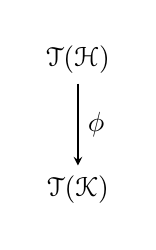
\begin{tikzpicture}
  \matrix (m) [matrix of math nodes,row sep=3em,column sep=2em,minimum width=1em]
  { 
    \mathcal{T}(\mathcal{H}) \\
     \mathcal{T}(\mathcal{K})  \\
  };
  \path[-stealth]
    (m-1-1) edge  node [right] {$\phi$} (m-2-1);
\end{tikzpicture}
\end{minipage}
\hspace{-50pt}
\begin{minipage}{0.45\textwidth}
\centering
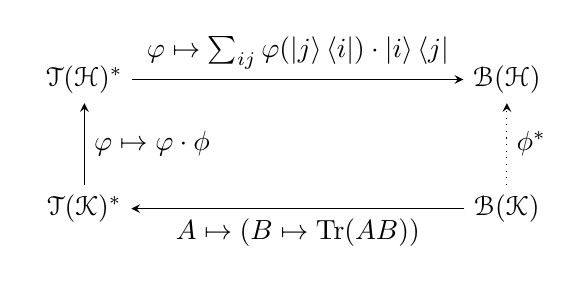
\begin{tikzpicture}
  \matrix (m) [matrix of math nodes,row sep=3em,column sep=12em,minimum width=1em]
  {
  \mathcal{T}(\mathcal{H})^*&  \mathcal{B}(\mathcal{H})  \\
   \mathcal{T}(\mathcal{K})^* &  \mathcal{B}(\mathcal{K}) \\
  };
  \path[-stealth]
    (m-1-1) edge  node [above] {$\varphi \mapsto \sum_{ij} \varphi(\ket{j}\bra{i}) \cdot \ket{i} \bra{j}  $} (m-1-2)
    (m-2-2) edge [dotted]  node [right] {$\phi^*$} (m-1-2)
    (m-2-2) edge  node [below] {$ A \mapsto (B \mapsto \tr(AB)) $} (m-2-1)
    (m-2-1) edge  node [right] {$ \varphi \mapsto \varphi \cdot \phi $} (m-1-1)
    ;
\end{tikzpicture}
\end{minipage}
\]


This means that the map $\phi^* : \mathcal{B}(\mathcal{K}) \to \mathcal{B}(\mathcal{H})$ can be defined as
\[
\phi^*(A) = \sum_{i,j} \operatorname{tr}\left(A \cdot \phi(\ket{j}\bra{i})\right) \cdot \ket{i}\bra{j},
\]
where \( i \) and \( j \) range over an orthonormal basis of \( \mathcal{H} \). 

Note that the map between spaces $\mathcal{T}(\mathcal{H})^*$ and $\mathcal{B}(\mathcal{H})$ is defined using the Riez Representation Theorem.

\begin{definition} [Riesz Representation Theorem]
Let $V$ be a finite-dimensional inner product space, and let $\varphi$ be a linear functional on $V$. Then there exists a unique vector $v_\varphi \in V$ such that
$$
\varphi(w) = \langle w, v_\varphi \rangle \quad \text{for all } w \in V.
$$
We call $v_\varphi$ the \emph{Riesz vector} for $\varphi$ and denote it by $v_\varphi$.\\
\end{definition}

Using the Riesz representation theorem, we can define a map 
$\phi^* : V^* \to V$
by setting \(\phi*(\varphi) = v_\varphi\), where \(v_\varphi\) is the Riesz vector corresponding to \(\varphi \in V^*\). Since the Riesz representation is unique, \(\phi^*\) is well-defined \cite{romanAdvancedLinearAlgebra1992}. 

Let $\sigma= n_1, \ldots, n_s$. For $\phi: \mathcal{M}_\sigma^* \to \mathcal{M}_\sigma $, by the Riesz representation theorem, we have
$$ \varphi(\ket{j} \bra{i})= \langle \ket{j} \bra{i},  v_\varphi  \rangle = \sum_{k=1}^s \langle \ket{j_k} \bra{i_k},  v_{\varphi,k}  \rangle = \sum_{k=1}^s  \tr \left( \ket{i_k} \bra{j_k} \cdot   v_{\varphi,k} \right) =  v_{\varphi,p_k,q_k} $$
where the subscript \(k\) refers to the \(k\)-th component of the vector \(v_\varphi\), and \(v_{\varphi, p_k, q_k}\) denotes the entry in the \(p_k\)-th column and \(q_k\)-th row of the matrix \(v_{\varphi,k}\). Note that when the set of orthonormal basis states of \(\mathbb{C}^{n_1} \oplus \ldots \oplus \mathbb{C}^{n_s}\) is decomposed by its components, all but one of the components are zero vectors this is the one we designate by $k$ in the last step.

As a result $\phi^*(\varphi) =  \sum_{ij} \varphi(\ket{j}\bra{i}) \cdot \ket{i} \bra{j} = \sum_{ij}  v_{\varphi,p_k,q_k} \cdot  \ket{i} \bra{j}  = v_{\varphi}$.



\begin{example}
  We now proceed to illustrate the aforementioned correspondence for specific operators $\phi$.
  \begin{enumerate}
    \item $\phi: \Complex \to \Complex^{2 \times 2}$, $ \phi(1)= \ket{\psi}\bra{\psi}$. In this case, $\phi^*:\Complex^{2 \times 2} \to \Complex$ is defined as  
    $$\phi^*(\rho) =  \tr\left( \rho \cdot \ket{\psi}\bra{\psi}\right).$$ 
    Note that for $S \in \Complex^{2 \times 2}$ and $T \in \Complex$, we have 
    $$\tr(\phi(T)\cdot S) =  T \cdot \tr\left(\ket{\psi}\bra{\psi}\right) \cdot S = \tr(T\cdot \phi^*(S)). $$

    \item $\phi: \Complex \oplus \Complex \to \Complex^{2 \times 2}$, $\phi((a,b))=\left(\begin{smallmatrix}
    a & 0 \\
    0 & b
  \end{smallmatrix}\right).$ 
  In this case, $\phi^*:\Complex^{2 \times 2} \to \Complex \oplus \Complex$ is defined as
    $$\phi^*\left( \begin{pmatrix}
    a & b \\
    c & d
    \end{pmatrix}\right) 
    = \left( \tr\left( \begin{pmatrix}
    a & b \\
    c & d
    \end{pmatrix}  \begin{pmatrix}
    1 & 0 \\
    0 & 0
    \end{pmatrix}\right),
     \tr\left( \begin{pmatrix}
    a & b \\
    c & d
    \end{pmatrix}  \begin{pmatrix}
    0 & 0 \\
    0 & 1
    \end{pmatrix}\right) \right)
    %= \left( \tr \begin{pmatrix}
    %a & 0 \\
    %c & 0
    %\end{pmatrix},\tr \begin{pmatrix}
    %0 & b \\
    %0 & d \end{pmatrix} \right) 
    = \left(a,d\right).$$
    Note that for all $S= \left(\begin{smallmatrix}
    a & b \\
    c & d
  \end{smallmatrix}\right). $ and $T = (x,y)$, we have 
    $$\tr(\phi(T)\cdot S) =   \tr\left(\begin{pmatrix}
    x & 0 \\
    0 & y
    \end{pmatrix}\cdot \begin{pmatrix}
    a & b \\
    c & d
    \end{pmatrix}\right) = x\cdot a + y \cdot d = \tr\left( (x,y) \cdot (a,d)\right) = \tr(T\cdot \phi^*(S)). $$


    \item $\phi: \Complex^{2 \times 2} \to  \Complex \oplus \Complex $, $\phi\left(\begin{smallmatrix}
    a & 0 \\
    0 & b
  \end{smallmatrix}\right) = (a,b).$  In this case, $\phi^*: \Complex \oplus \Complex \to \Complex^{2 \times 2}  $ is defined as
    $$\phi^*\left( (a,b)\right) 
    = \tr ((a,b) \cdot (1,0)) \cdot \ket{0}\bra{0} + \tr ((a,b) \cdot (0,1)) \cdot \ket{1}\bra{1}
    = \begin{pmatrix}
    a & 0 \\
    0 & b
    \end{pmatrix}.$$
    Note that for all and $S = (a,b)$ and $T= \left(\begin{smallmatrix}
    x & y \\
    w & z
  \end{smallmatrix}\right)$, we have 
    $$\tr(\phi(T)\cdot S) = \tr\left( (x,z) \cdot (a,b)\right) = x\cdot a + y\cdot b =  \tr\left(\begin{pmatrix}
    x & y \\
    w & z
    \end{pmatrix}\cdot \begin{pmatrix}
    a & 0 \\
    0 & d
    \end{pmatrix}\right)  = \tr(T\cdot \phi^*(S)). $$
    
  \item  $\phi: \Complex^{2 \times 2} \to  \Complex \oplus \Complex $, $\phi(\rho) = T \rho T^\dag,$ with $T = \left(\begin{smallmatrix}
    1 & 0 \\
    0 & e^{-i \pi/4}
  \end{smallmatrix}\right).$ In this case, $\phi^*: \Complex^{2 \times 2} \to \Complex^{2 \times 2}  $ is defined as
    $$\phi^*\left( \rho\right) 
    = T^\dag \rho T$$
    Note that for all and $S = \left(\begin{smallmatrix}
    a & b \\
    c & d
  \end{smallmatrix}\right)$ and $T= \left(\begin{smallmatrix}
    x & y \\
    w & z
  \end{smallmatrix}\right)$, we have 
  \begin{align*}
    \tr(\phi(T)\cdot S) &= \tr\left(\begin{pmatrix}
    x & y\cdot e^{i \pi/4} \\
    w \cdot e^{-i \pi/4} & z
    \end{pmatrix}\cdot \begin{pmatrix}
    a & b \\
    c & d
    \end{pmatrix}\right) \\
    &= x\cdot a + y \cdot c \cdot e^{i \pi/4} + w\cdot b \cdot e^{-i\pi/4} + z \cdot d \\
    &= \tr\left(\begin{pmatrix}
    x & y \\
    w  & z
    \end{pmatrix}\cdot \begin{pmatrix}
    a & b\cdot e^{-i \pi/4} \\
    c \cdot e^{i \pi/4} & d
    \end{pmatrix}\right) = \tr(T\cdot \phi^*(S)).
  \end{align*}

  \item  $\phi: \Complex^{2 \times 2} \to  \Complex \oplus \Complex $, $\phi( \left(\begin{smallmatrix}
    a & b \\
    c & d
  \end{smallmatrix}\right)) = \left(\begin{smallmatrix}
    a+d & 0 \\
    0 & 0
  \end{smallmatrix}\right).$ In this case, $\phi^*: \Complex^{2 \times 2} \to \Complex^{2 \times 2}  $ is defined as
    $$\phi^*\left( \begin{pmatrix}
    a & b \\
    c & d
  \end{pmatrix}\right) 
    =  \tr \left(\begin{pmatrix}
    a & b \\
    c & d
  \end{pmatrix}\begin{pmatrix}
    1 & 0 \\
    0 & 0
  \end{pmatrix}\right) \begin{pmatrix}
    1 & 0 \\
    0 & 0
  \end{pmatrix}  
  + \tr \left(\begin{pmatrix}
    a & b \\
    c & d
  \end{pmatrix}\begin{pmatrix}
    1 & 0 \\
    0 & 0
  \end{pmatrix}\right) \begin{pmatrix}
    0 & 0 \\
    0 & 1
  \end{pmatrix} 
  = \begin{pmatrix}
    a & 0 \\
    0 & a
  \end{pmatrix}  $$
 Note that for all and $S = \left(\begin{smallmatrix}
    a & b \\
    c & d
  \end{smallmatrix}\right)$ and $T= \left(\begin{smallmatrix}
    x & y \\
    w & z
  \end{smallmatrix}\right)$, we have 
  \begin{align*}
    \tr(\phi(T)\cdot S) &= \tr\left(\begin{pmatrix}
    x +z& 0 \\
    0 & 0
    \end{pmatrix}\cdot \begin{pmatrix}
    a & b \\
    c & d
    \end{pmatrix}\right) =(x+z)\cdot a  = \tr\left(\begin{pmatrix}
    x & y \\
    w  & z
    \end{pmatrix}\cdot \begin{pmatrix}
    a & 0 \\
    0 & a
    \end{pmatrix}\right) = \tr(T\cdot \phi^*(S)).
  \end{align*}

  \end{enumerate}
\end{example}



The category  $\WstarCPSUop$ is a model of the metric $\lambda$-theory for quantum computation under the following interpretation: 
$\sem{\typeI}$, 
$\sem{\emph{qbit} \hspace{1pt}}$, $\sem{\emph{q} \hspace{1pt}}$, $\sem{\ket{\psi}}$ for $\psi \in \{0, 1\}$, $\sem{\emph{meas}}$ and $\sem{U}$ are ``imported from'' $\catQ$. To these we add $\sem{\emph{pos} \hspace{1pt}}= \mathcal{B}(\ell^2(\mathbb{Z}))$ and $\sem{S}= \rho \mapsto S \rho \, S^\dag$.

Note that in the infinite-dimensional setting (for separable Hilbert spaces), unitary transformations of the form $\rho \mapsto U \rho U^\dag$ are still quantum channels, and are therefore completely positive and unital by definition \cite[Example~4.6, Definition~1.48]{heinosaariMathematicalLanguageQuantum2011}. 

\todo[inline]{Questão modelo: Para termos medições em espaços infinitos teríamos de ter produtos infinitos? Also a questão da medição ser cpu é clean se for a medição tradicional da que temos tinha de provar à pata (em principio)}
\todo[inline]{Ou seja não vou usar medições}
%The same applies to measurements given they are channels and unital \cite[Proposition~4.21]{heinosaariMathematicalLanguageQuantum2011}.





%\bar{\otimes} 



% defs (ops sytem)
% teoremas
%3.6
%8.2
%12.3
%3.2.2 (op spaces)
%prova





  \end{example}
  



\newpage
\bibliographystyle{alpha} 
\bibliography{biblio}
\end{document}
